\chapter{2020 Near Detector Fit Results}\label{sec:2020Fit}

The results of the analysis are presented in this Chapter, starting with the nominal MC prediction and fit validations in Sections \ref{sec:nommc}, \ref{sec:llhscan}, \ref{sec:sigvar}, and \ref{sec:asimov}. The data fit is presented in \ref{sec:datafit}, and the posterior predictive distributions and p values are are shown in \ref{sec:postpred}. Results from fits with updated binnings are then compared in Section \ref{sec:newbin}.

\section{Nominal MC}\label{sec:nommc}

The data, unweighted MC, and nominal MC event rates for each sample are shown in Table \ref{tab:nomrates}. The CC 0$\pi$ samples are consistently underestimated in the MC prediction by $\sim$20$\%$, the CC 1$\pi$ samples are overestimated by $\sim$10$\%$ for FHC and underestimated by $\sim$5-10$\%$ for RHC, and the CC Other samples are underestimated by $\sim$20-30$\%$. The differences to data are consistent across to the FGDs to within $\sim$2$\%$. Overall, the MC prediction is $16\%$ lower than the observed data.

\begin{center}
\begin{table}[h]
\center
\begin{tabular}{l||c|c|c|c}
\hline \hline
\textbf{Sample} & \textbf{Raw MC} & \textbf{Nominal MC} & \textbf{Data} & \textbf{Data/MC} \\
\hline
\hline
\textbf{FGD1 FHC $\nu$ CC 0$\pi$} & 524093 & 27951.1 & 33443 & 1.20 \\ 
\textbf{FGD1 FHC $\nu$ CC 1$\pi$} & 127176 & 8358.97 & 7713 & 0.92 \\ 
\textbf{FGD1 FHC $\nu$ CC Other} & 99730 & 7031.47 & 8026 & 1.14 \\ \hline
\textbf{FGD2 FHC $\nu$ CC 0$\pi$} & 521757 & 27556.2 & 33156 & 1.20 \\
\textbf{FGD2 FHC $\nu$ CC 1$\pi$} & 103305 & 6723.98 & 6281 & 0.93\\
\textbf{FGD2 FHC $\nu$ CC Other} & 94164 & 6454.68 & 7700 & 1.19 \\ \hline
\textbf{FGD1 RHC $\bar{\nu}$ CC 0$\pi$} & 115456 & 6980.48 & 8388 & 1.20\\
\textbf{FGD1 RHC $\bar{\nu}$ CC 1$\pi$} & 9272 & 668.897 & 698 & 1.04\\
\textbf{FGD1 RHC $\bar{\nu}$ CC Other} & 16790 & 1230.34 & 1472 & 1.20\\ \hline
\textbf{FGD2 RHC $\bar{\nu}$ CC 0$\pi$} & 112390 & 6771.47 & 8334 & 1.23\\
\textbf{FGD2 RHC $\bar{\nu}$ CC 1$\pi$} & 8533 & 603.301 & 650 & 1.08\\
\textbf{FGD2 RHC $\bar{\nu}$ CC Other} & 15616 & 1135.13 & 1335 & 1.18\\ \hline
\textbf{FGD1 RHC $\nu$ CC 0$\pi$} & 41789 & 2916.3 & 3594 & 1.23\\
\textbf{FGD1 RHC $\nu$ CC 1$\pi$} & 14304 & 1115.99 & 1111 & 1.00\\
\textbf{FGD1 RHC $\nu$ CC Other} & 12733 & 1031.87 & 1344 & 1.30\\ \hline
\textbf{FGD2 RHC $\nu$ CC 0$\pi$} & 41554 & 2901.65 & 3433 & 1.18\\
\textbf{FGD2 RHC $\nu$ CC 1$\pi$} & 11472 & 898.111 & 926 & 1.03\\ 
\textbf{FGD2 RHC $\nu$ CC Other} & 11954 & 962.735 & 1245 & 1.29\\ \hline
\textbf{Total} & 1882090 & 111293 & 128849 & 1.16\\ \hline\hline
\end{tabular}
\caption{MC and data event rates for the ND280 samples.}
\label{tab:nomrates}
\end{table}
\end{center}
The 2D nominal MC distributions are shown in Figure \ref{fig:2dnom}. The uniform-rectangular binning described in Section \ref{sec:binning} is used for the initial fits. 

\begin{figure}
\centering
\begin{subfigure}{.32\textwidth}
  \centering
  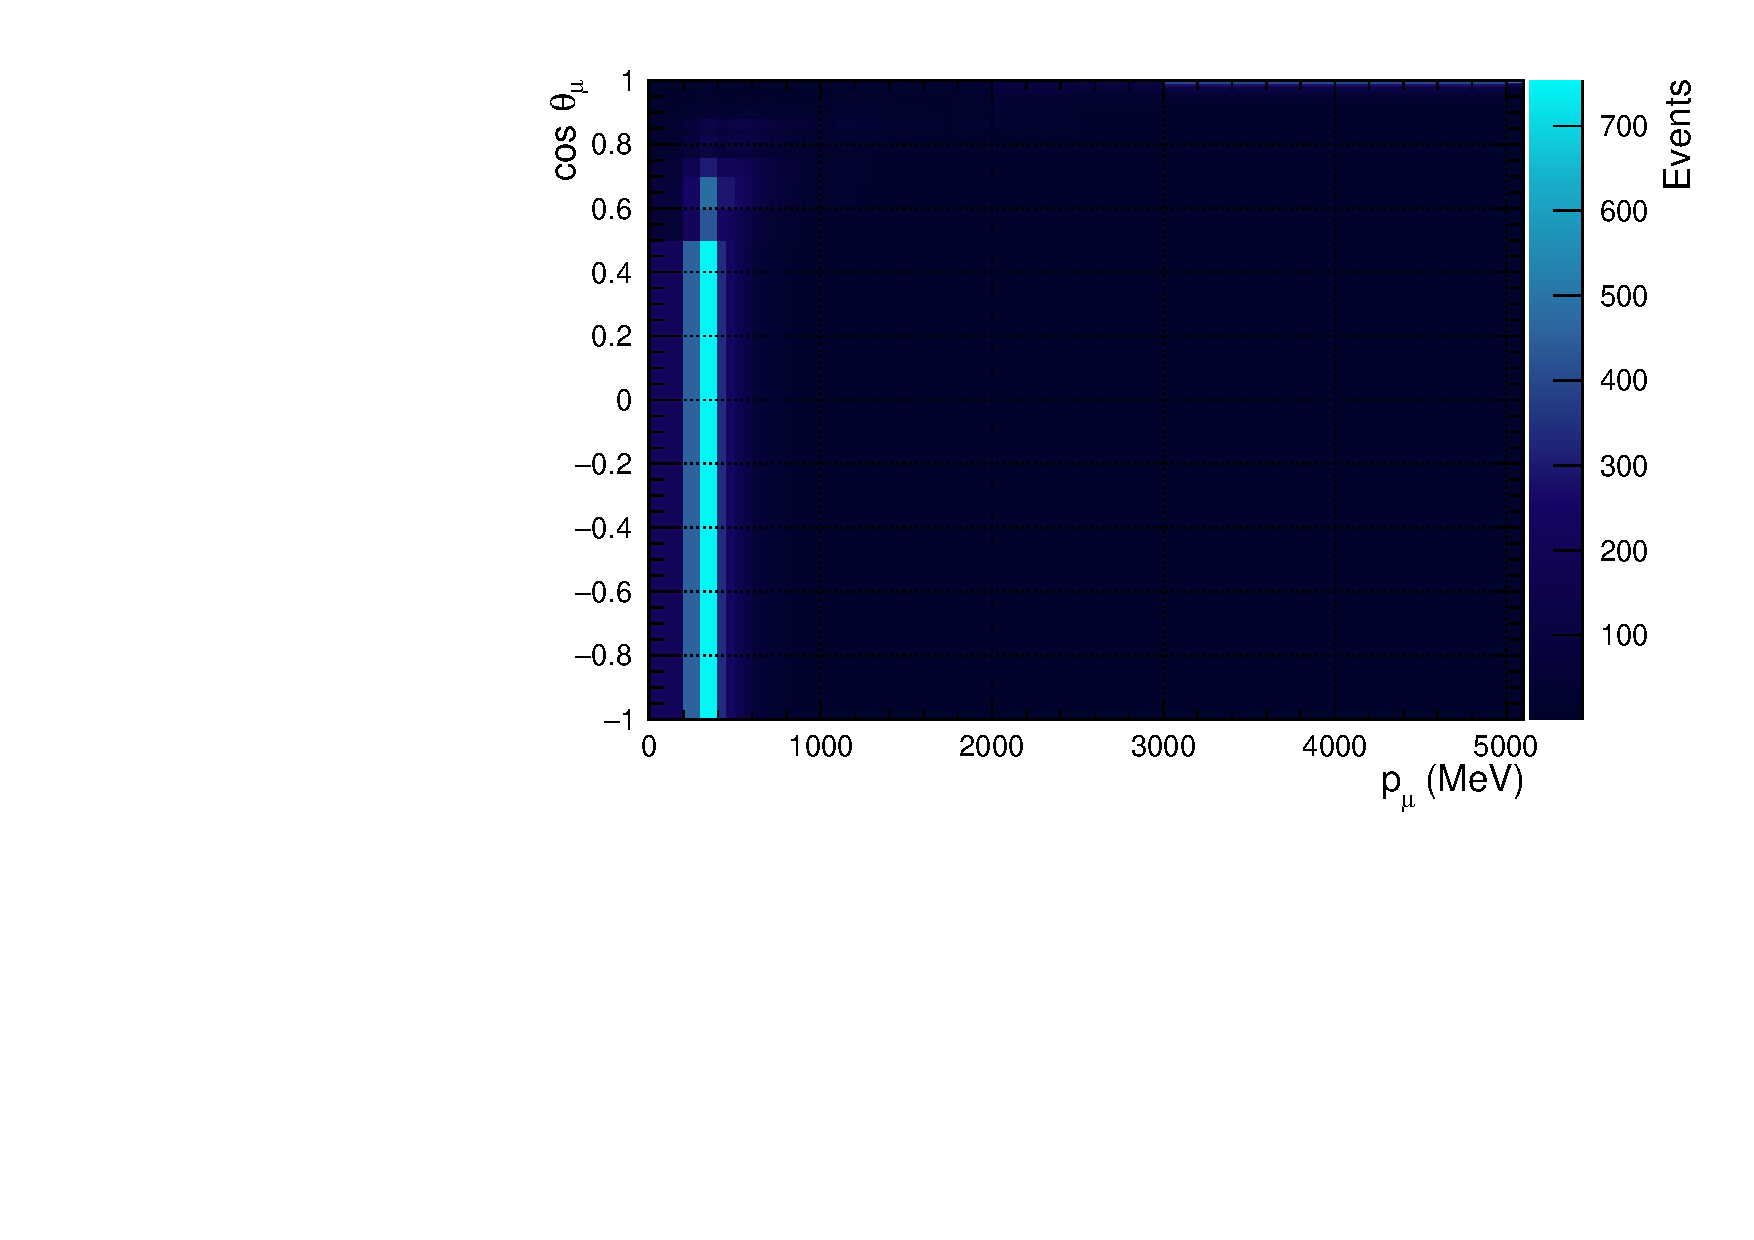
\includegraphics[width=0.95\linewidth]{figs/NomMC_MC_FGD1_numuCC_0pi}
  \caption{FGD1 FHC $\nu_{\mu}$ 0$\pi$}
  \label{fig:2d_FGD1_numuCC_0pi}
\end{subfigure}
\begin{subfigure}{.32\textwidth}
  \centering
  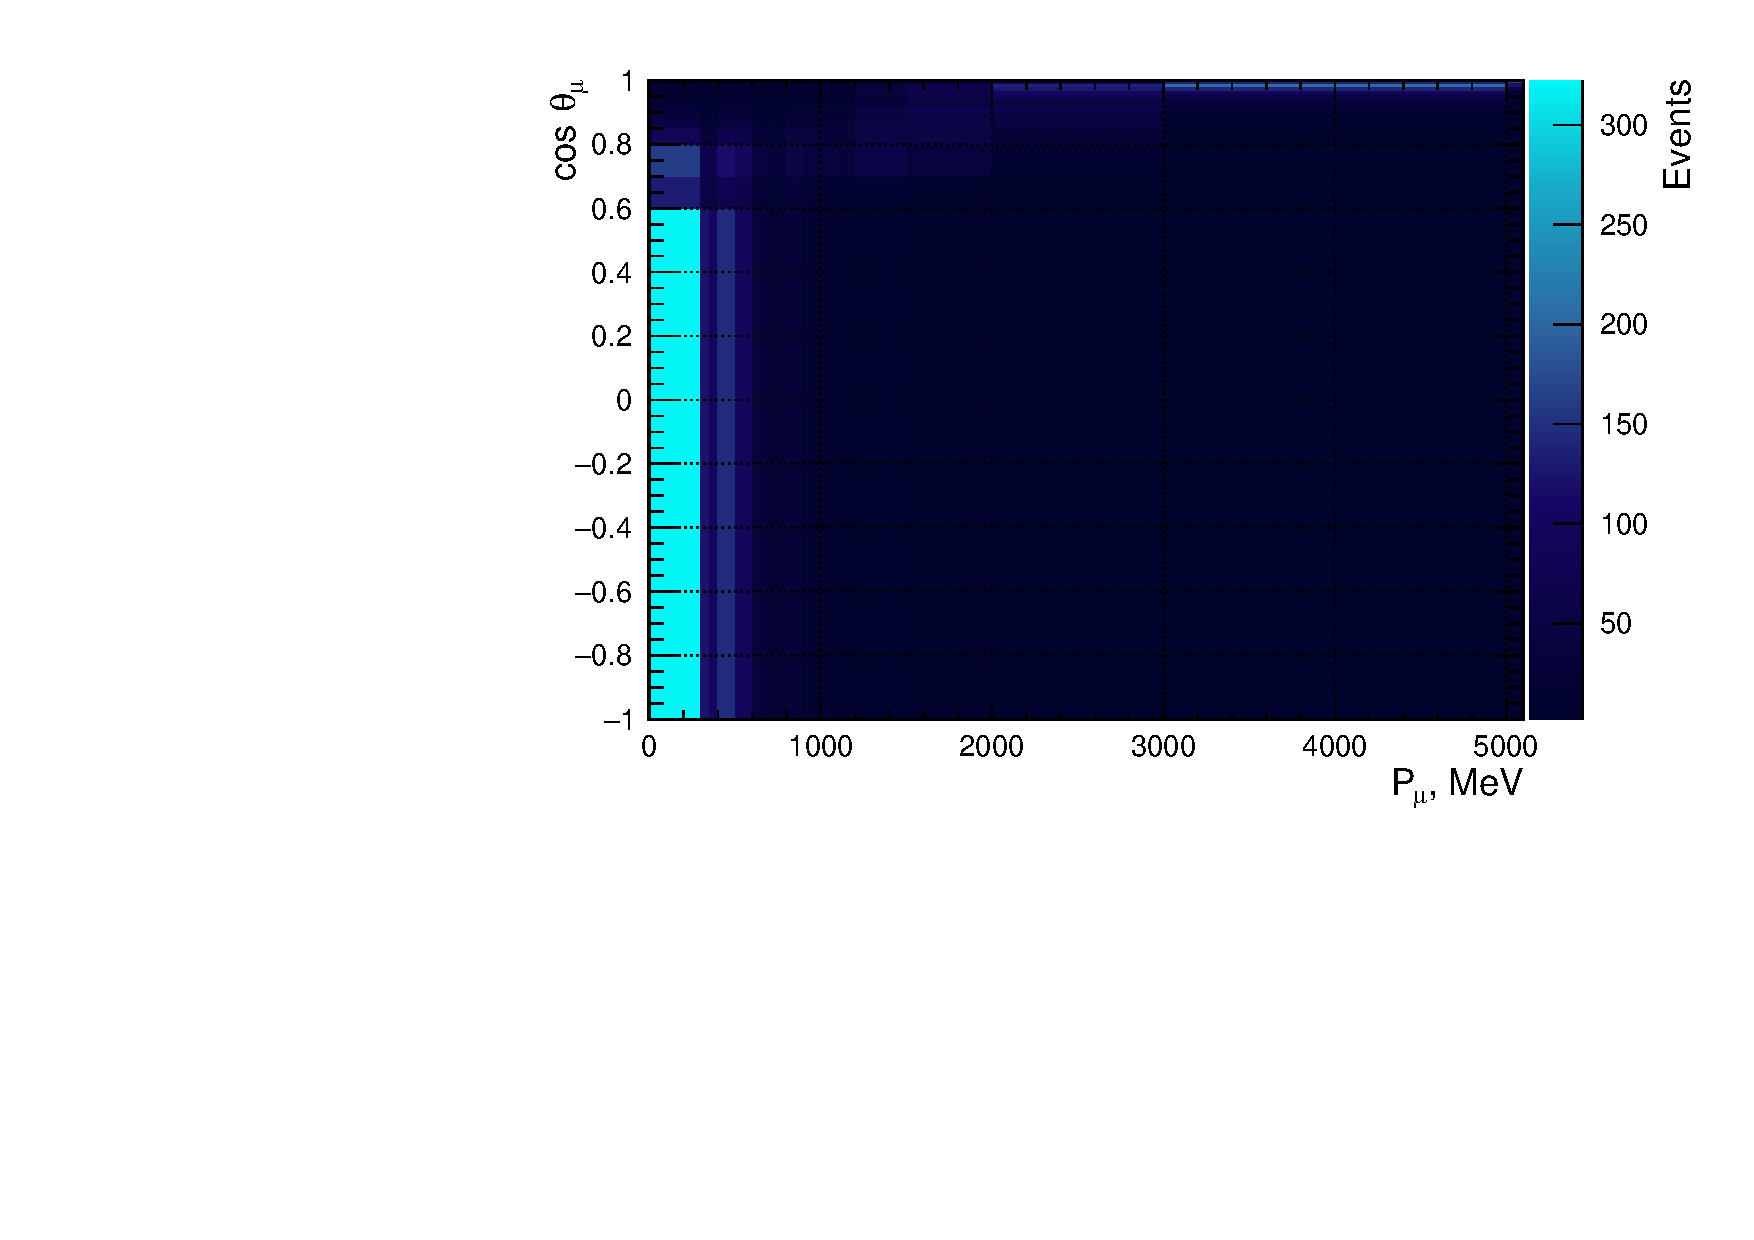
\includegraphics[width=0.95\linewidth]{figs/NomMC_MC_FGD1_numuCC_1pi}
  \caption{FGD1 FHC $\nu_{\mu}$ 1$\pi$}
  \label{fig:2d_FGD1_numuCC_1pi}
\end{subfigure}
\begin{subfigure}{.32\textwidth}
  \centering
  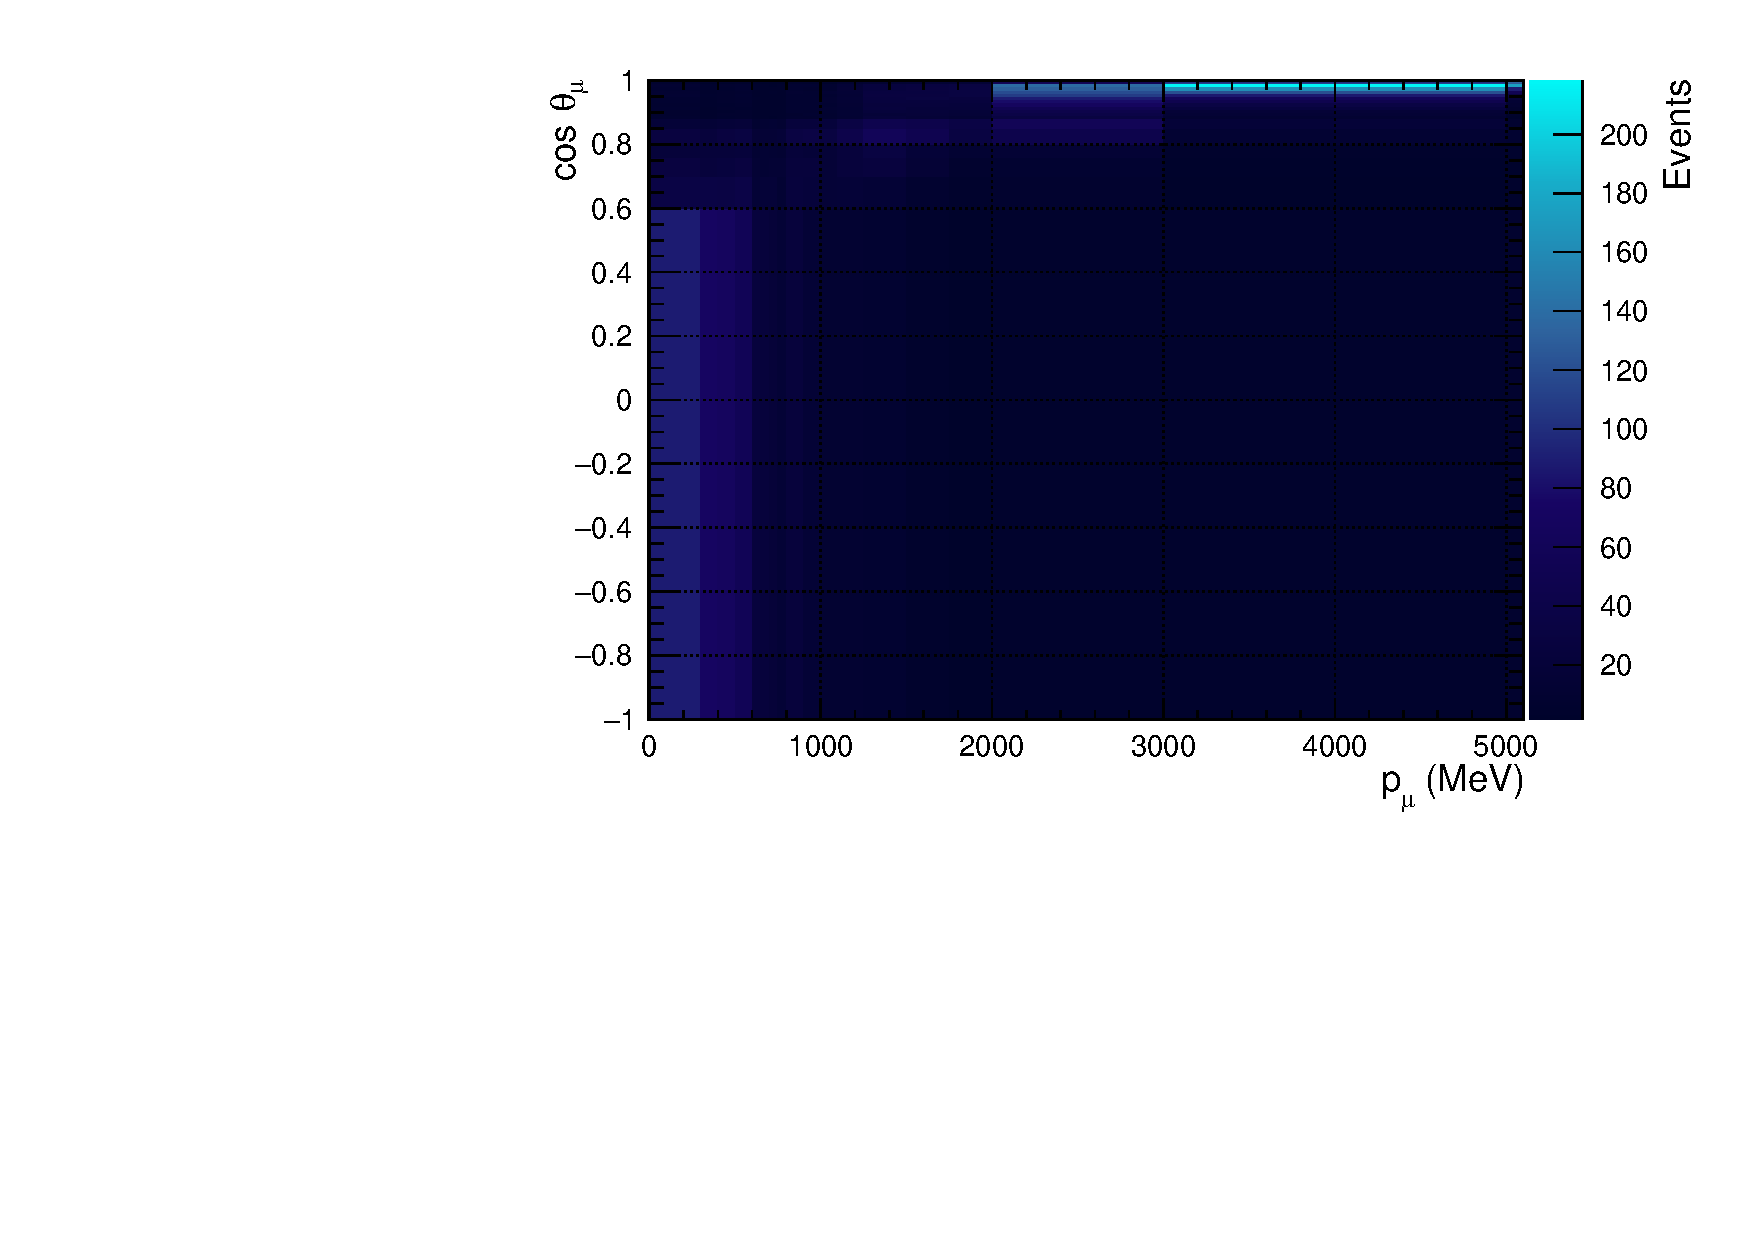
\includegraphics[width=0.95\linewidth]{figs/NomMC_MC_FGD1_numuCC_other}
  \caption{FGD1 FHC $\nu_{\mu}$ Other}
  \label{fig:2d_FGD1_numuCC_other}
\end{subfigure}
\centering
\begin{subfigure}{.32\textwidth}
  \centering
  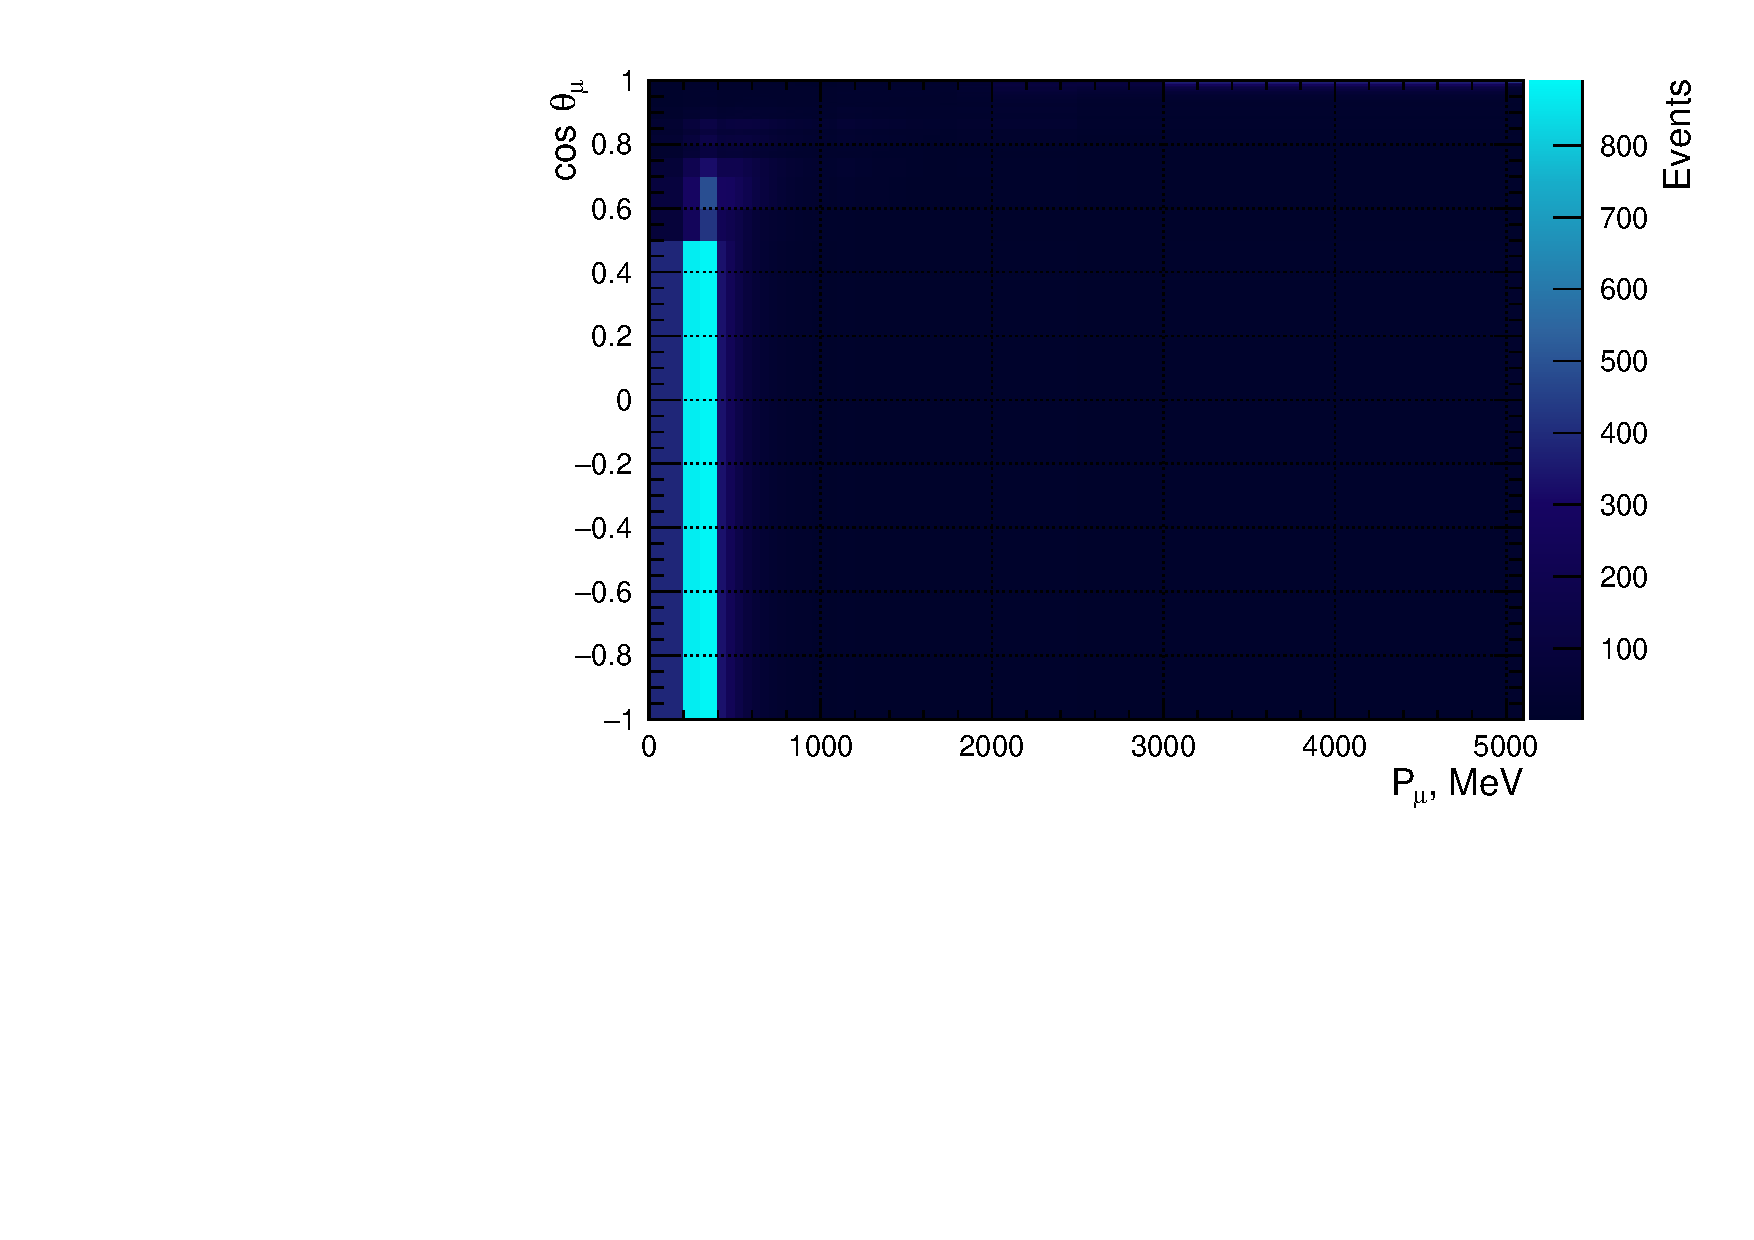
\includegraphics[width=0.95\linewidth]{figs/NomMC_MC_FGD2_numuCC_0pi}
  \caption{FGD2 FHC $\nu_{\mu}$ 0$\pi$}
  \label{fig:2d_FGD2_numuCC_0pi}
\end{subfigure}
\begin{subfigure}{.32\textwidth}
  \centering
  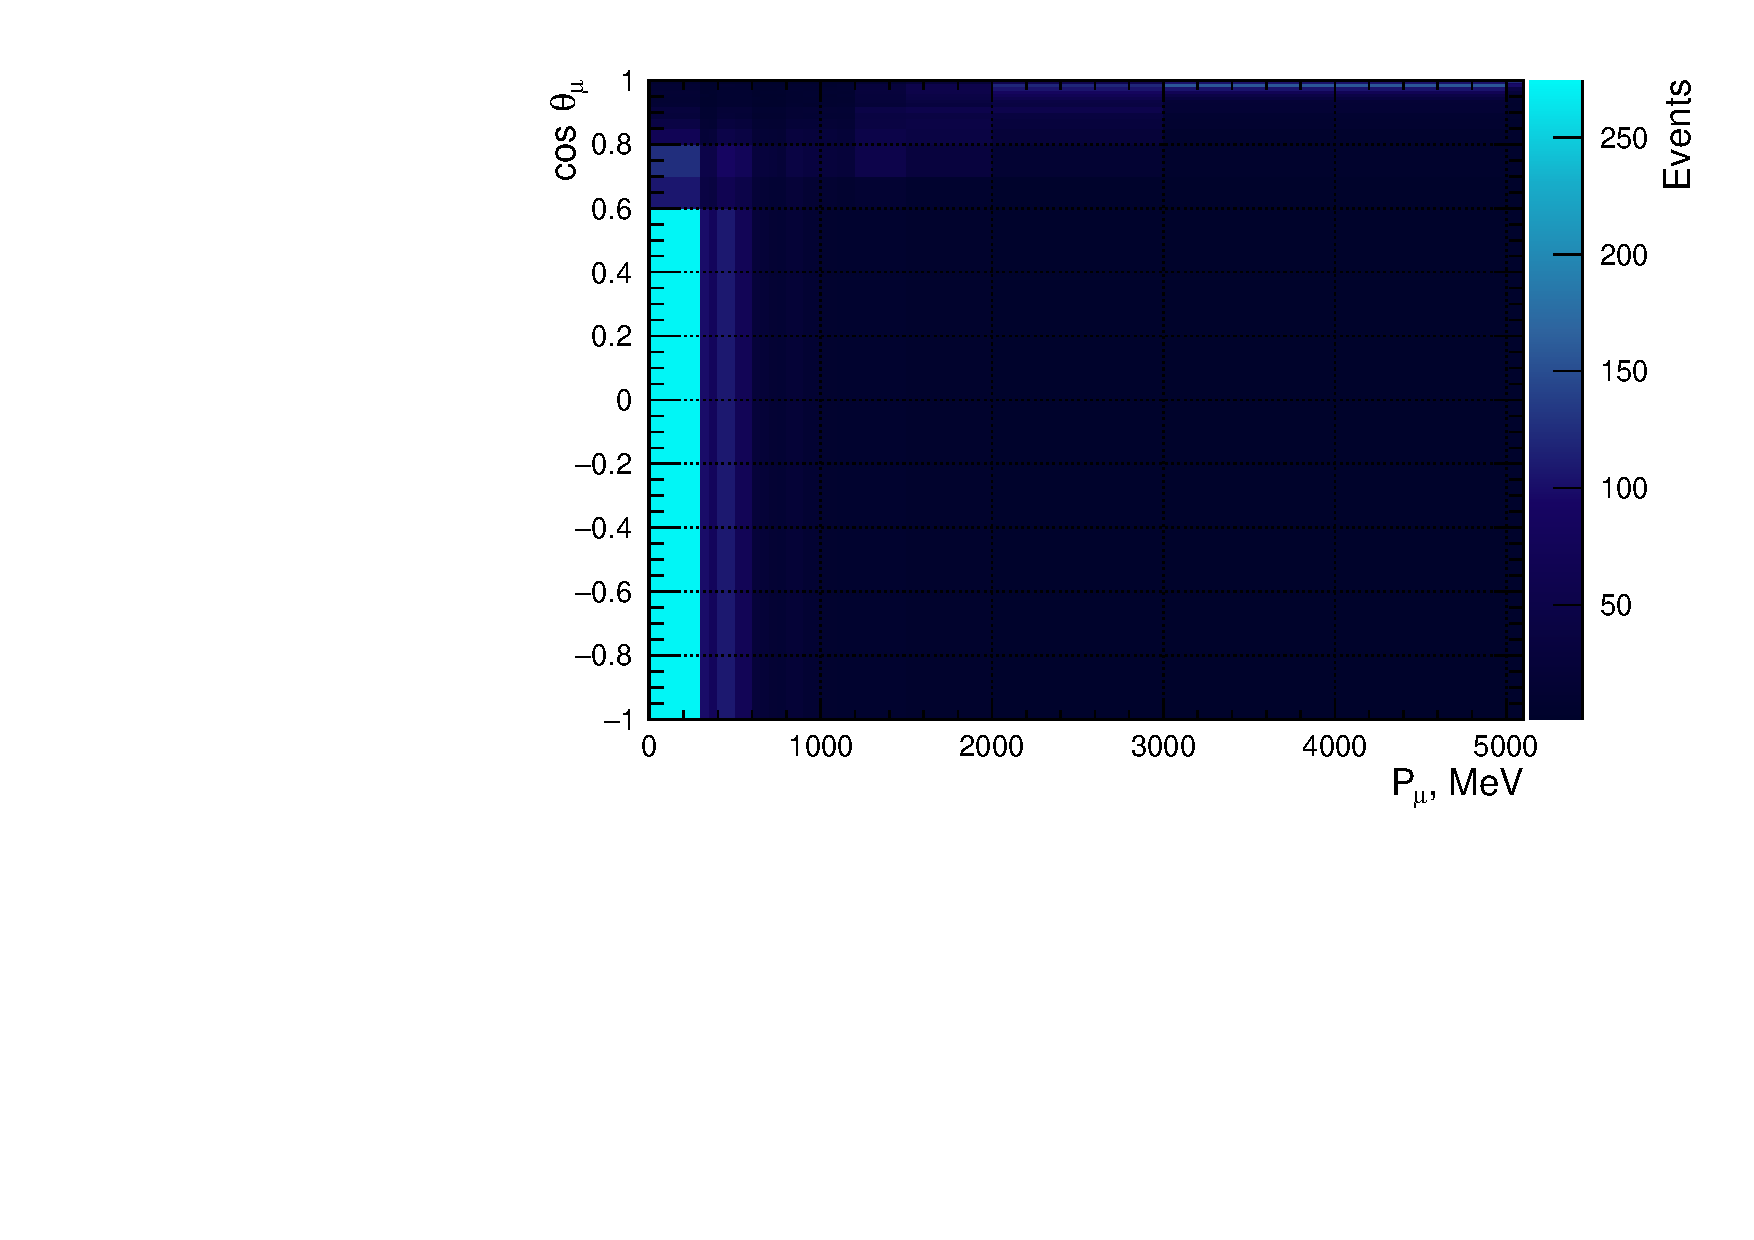
\includegraphics[width=0.95\linewidth]{figs/NomMC_MC_FGD2_numuCC_1pi}
  \caption{FGD2 FHC $\nu_{\mu}$ 1$\pi$}
  \label{fig:2d_FGD2_numuCC_1pi}
\end{subfigure}
\begin{subfigure}{.32\textwidth}
  \centering
  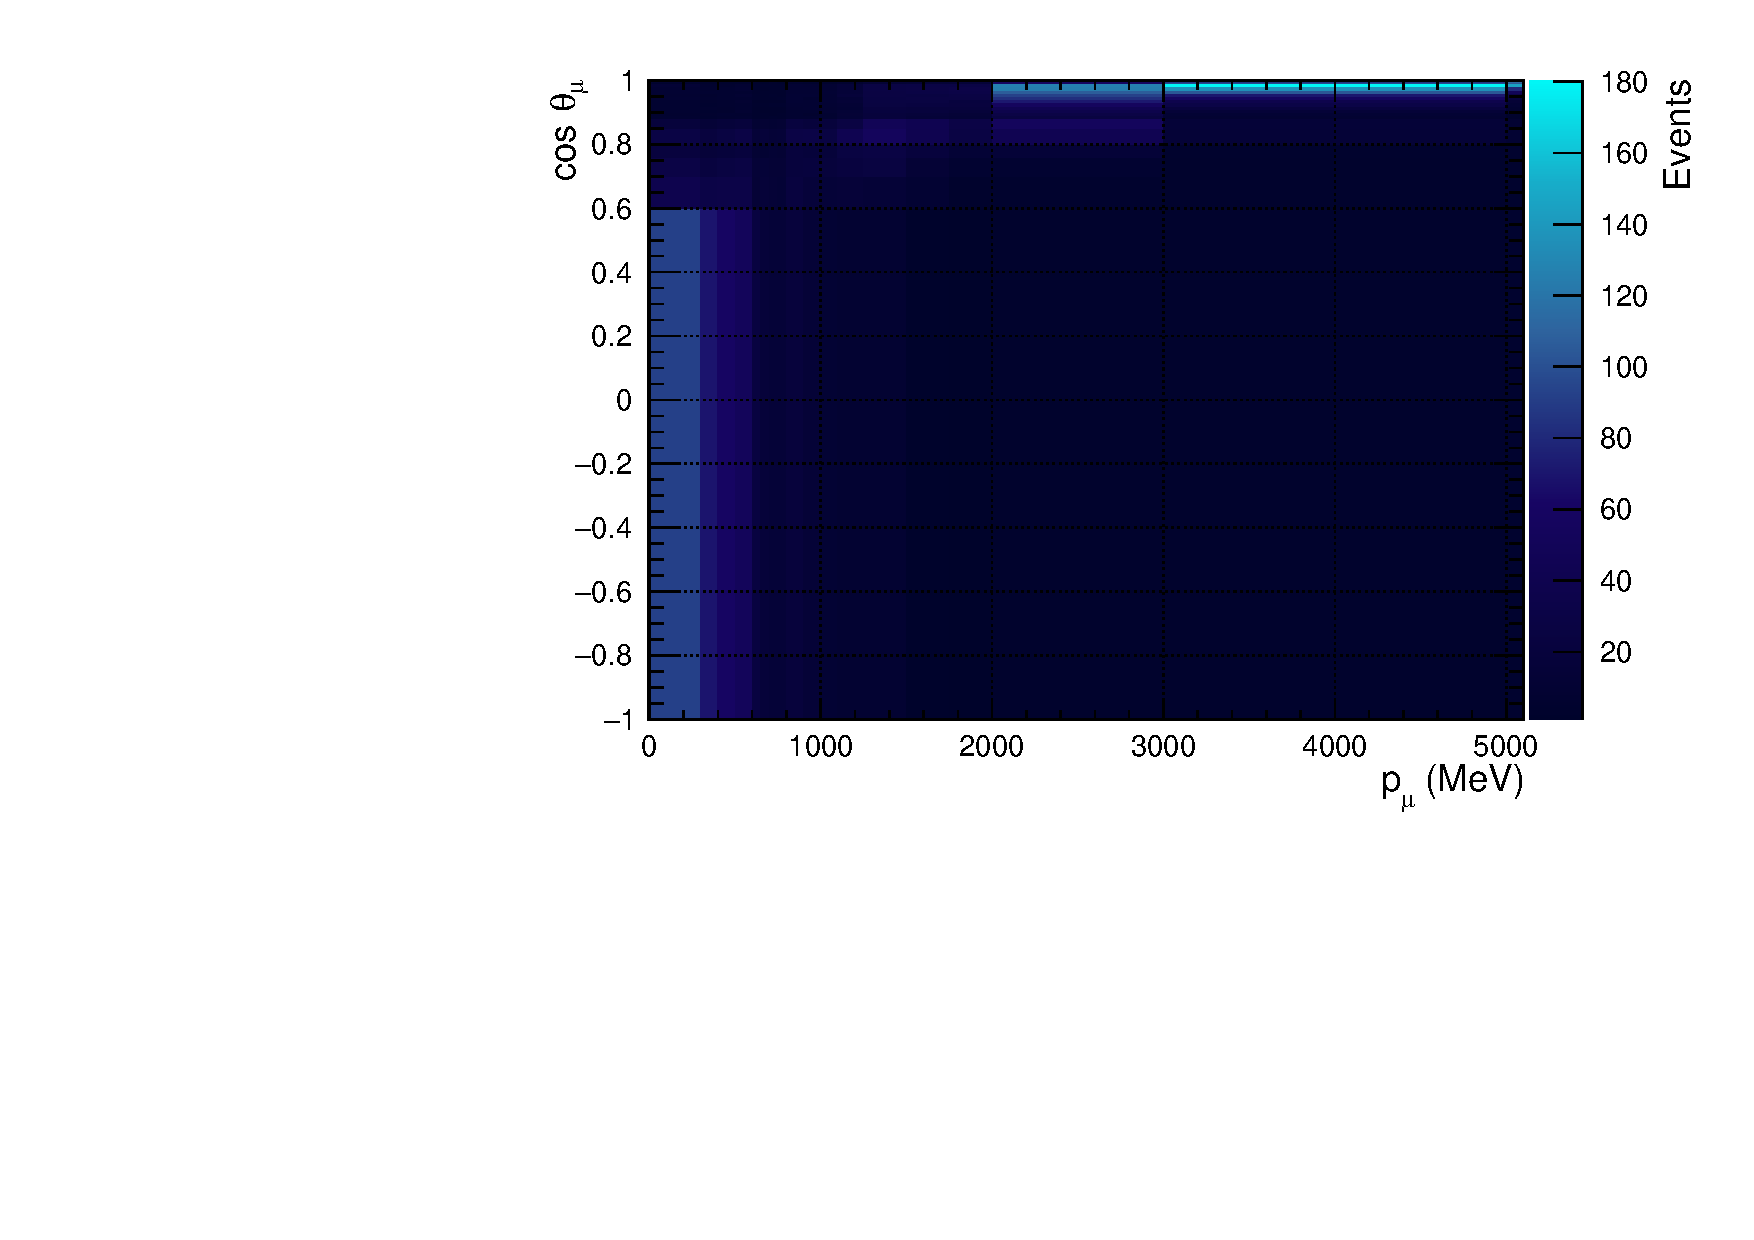
\includegraphics[width=0.95\linewidth]{figs/NomMC_MC_FGD2_numuCC_other}
  \caption{FGD2 FHC $\nu_{\mu}$ Other}
  \label{fig:2d_FGD2_numuCC_other}
\end{subfigure}
\centering
\begin{subfigure}{.32\textwidth}
  \centering
  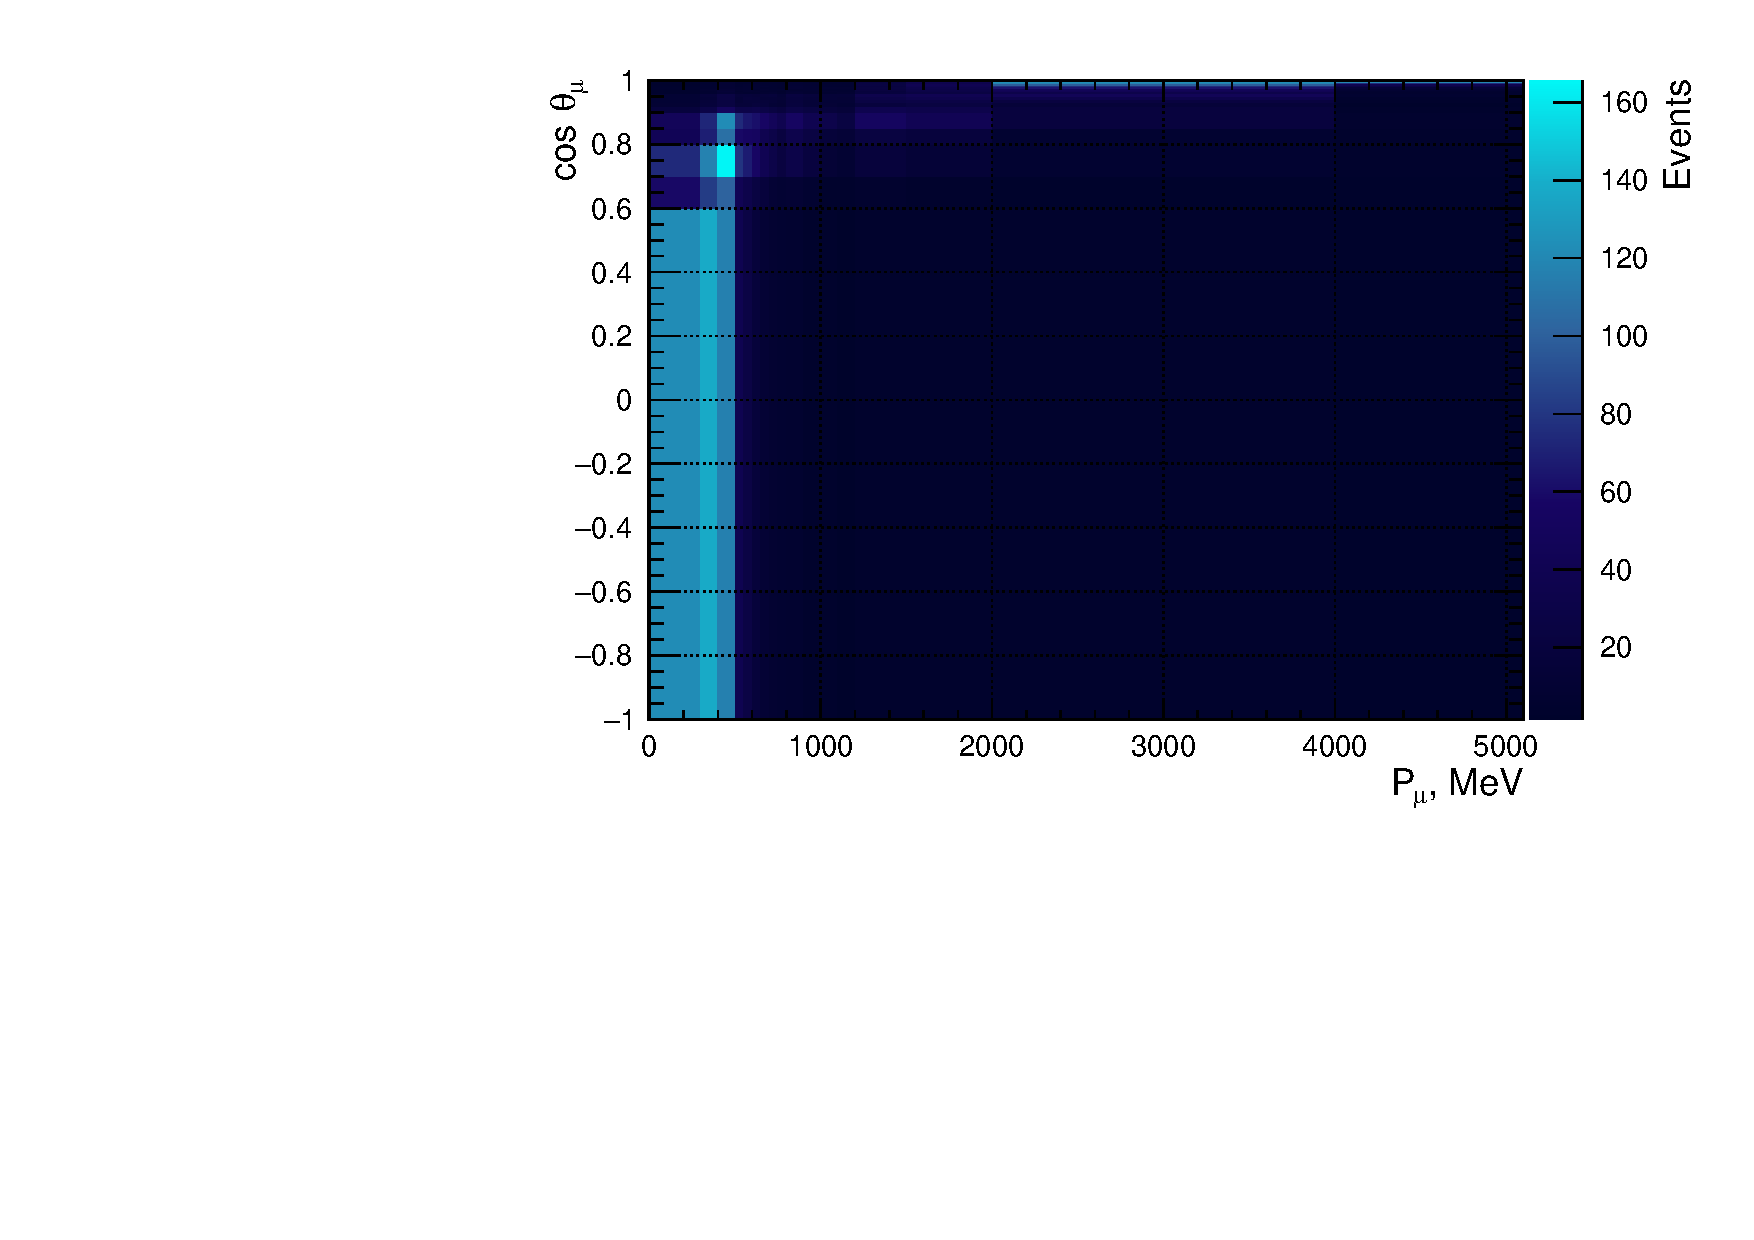
\includegraphics[width=0.95\linewidth]{figs/NomMC_MC_FGD1_anti-numuCC_0pi}
  \caption{FGD1 RHC $\bar{\nu_{\mu}}$ 0$\pi$}
  \label{fig:2d_FGD1_anti-numuCC_0pi}
\end{subfigure}
\begin{subfigure}{.32\textwidth}
  \centering
  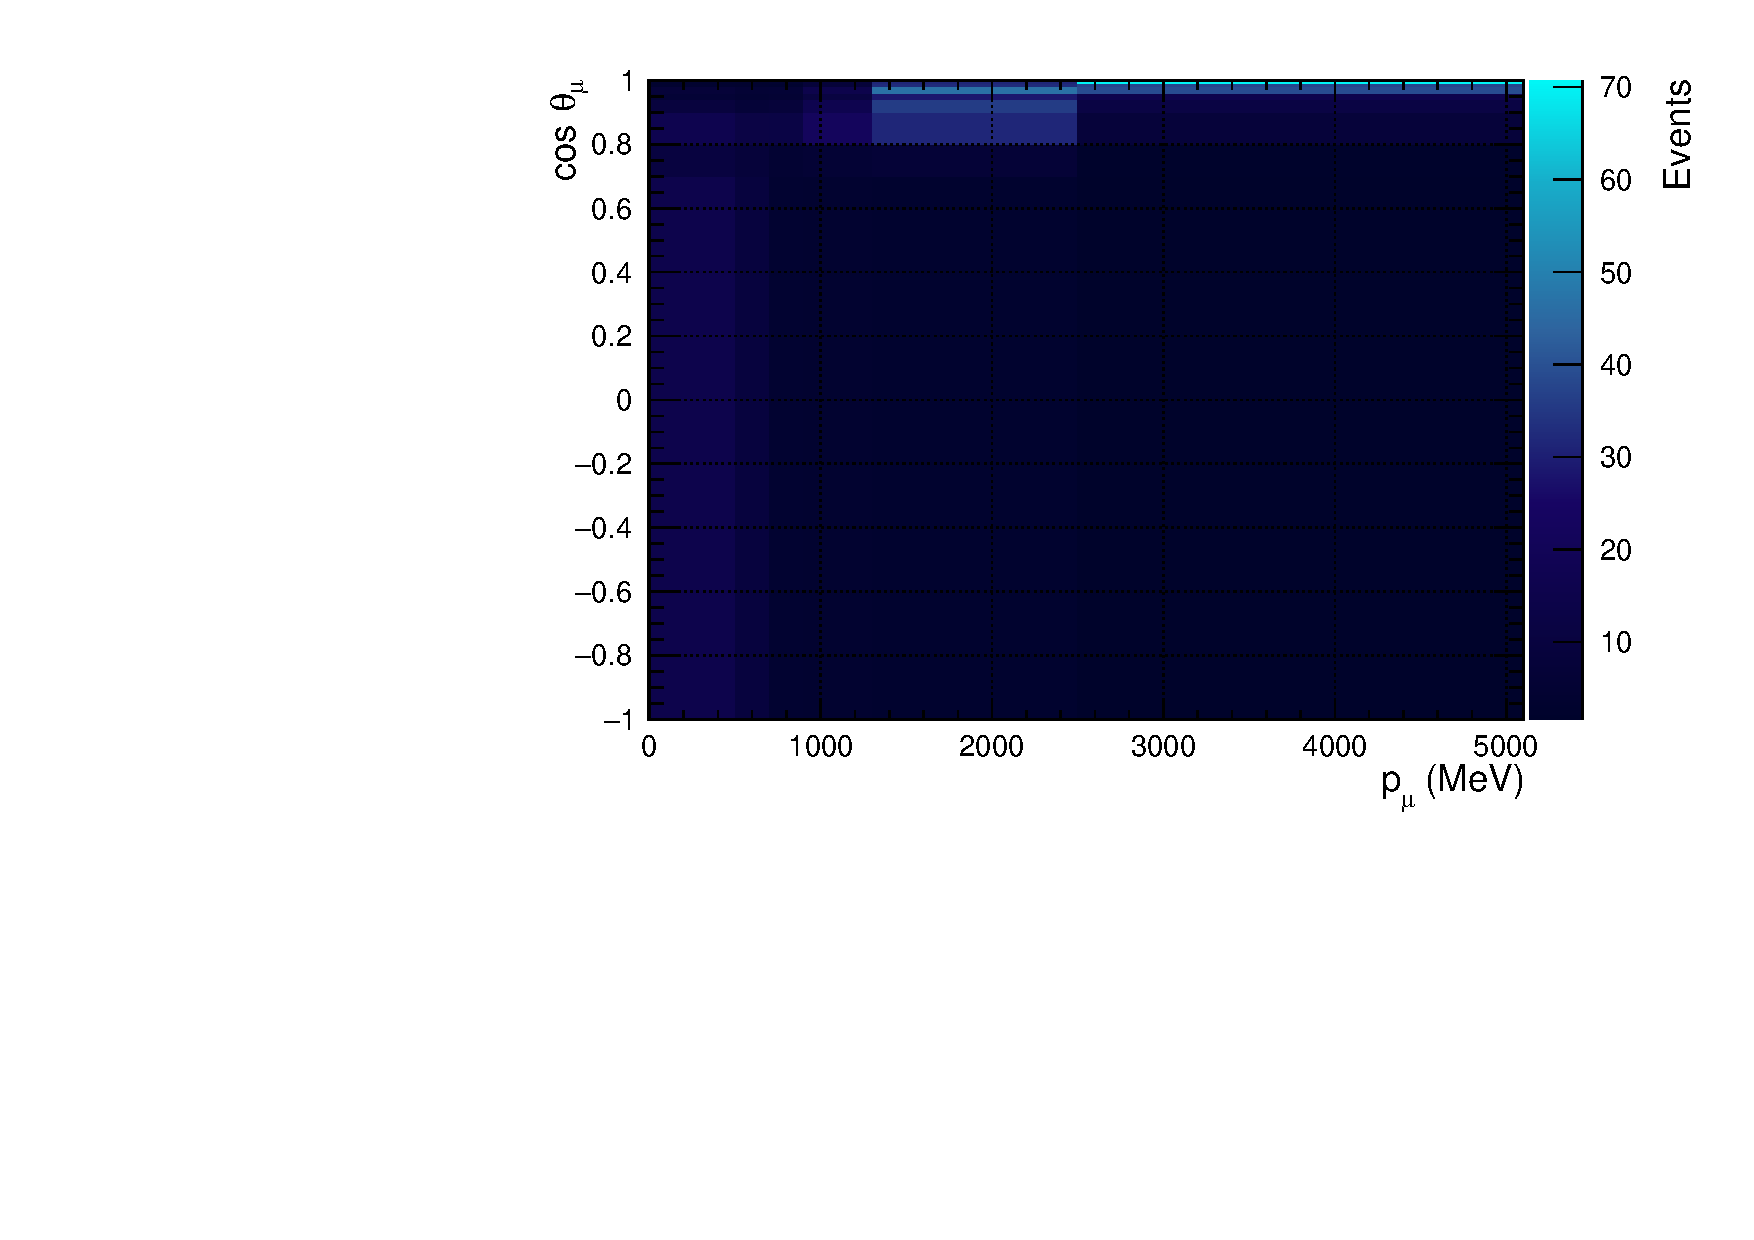
\includegraphics[width=0.95\linewidth]{figs/NomMC_MC_FGD1_anti-numuCC_1pi}
  \caption{FGD1 RHC $\bar{\nu_{\mu}}$ 1$\pi$}
  \label{fig:2d_FGD1_anti-numuCC_1pi}
\end{subfigure}
\begin{subfigure}{.32\textwidth}
  \centering
  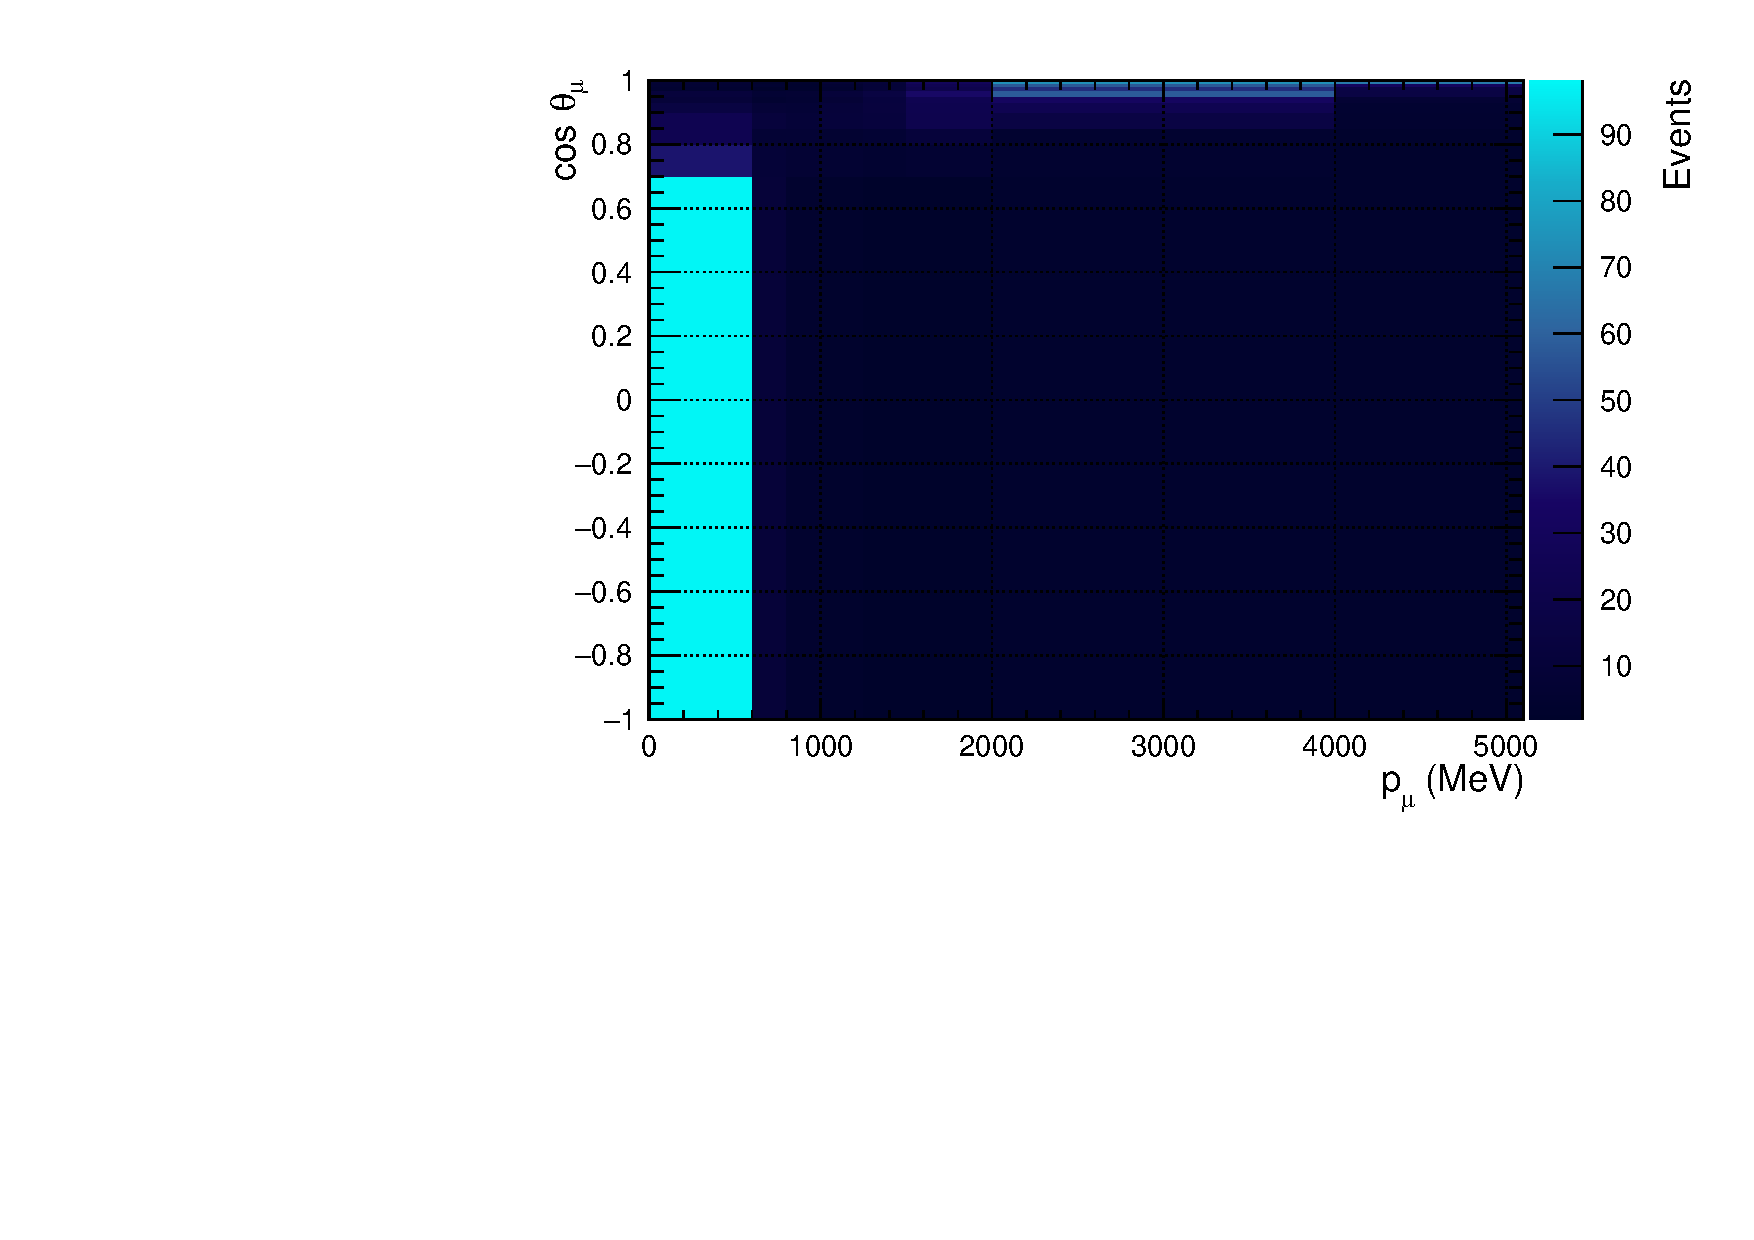
\includegraphics[width=0.95\linewidth]{figs/NomMC_MC_FGD1_anti-numuCC_other}
  \caption{FGD1 RHC $\bar{\nu_{\mu}}$ Other}
  \label{fig:2d_FGD1_anti-numuCC_other}
\end{subfigure}
\centering
\begin{subfigure}{.32\textwidth}
  \centering
  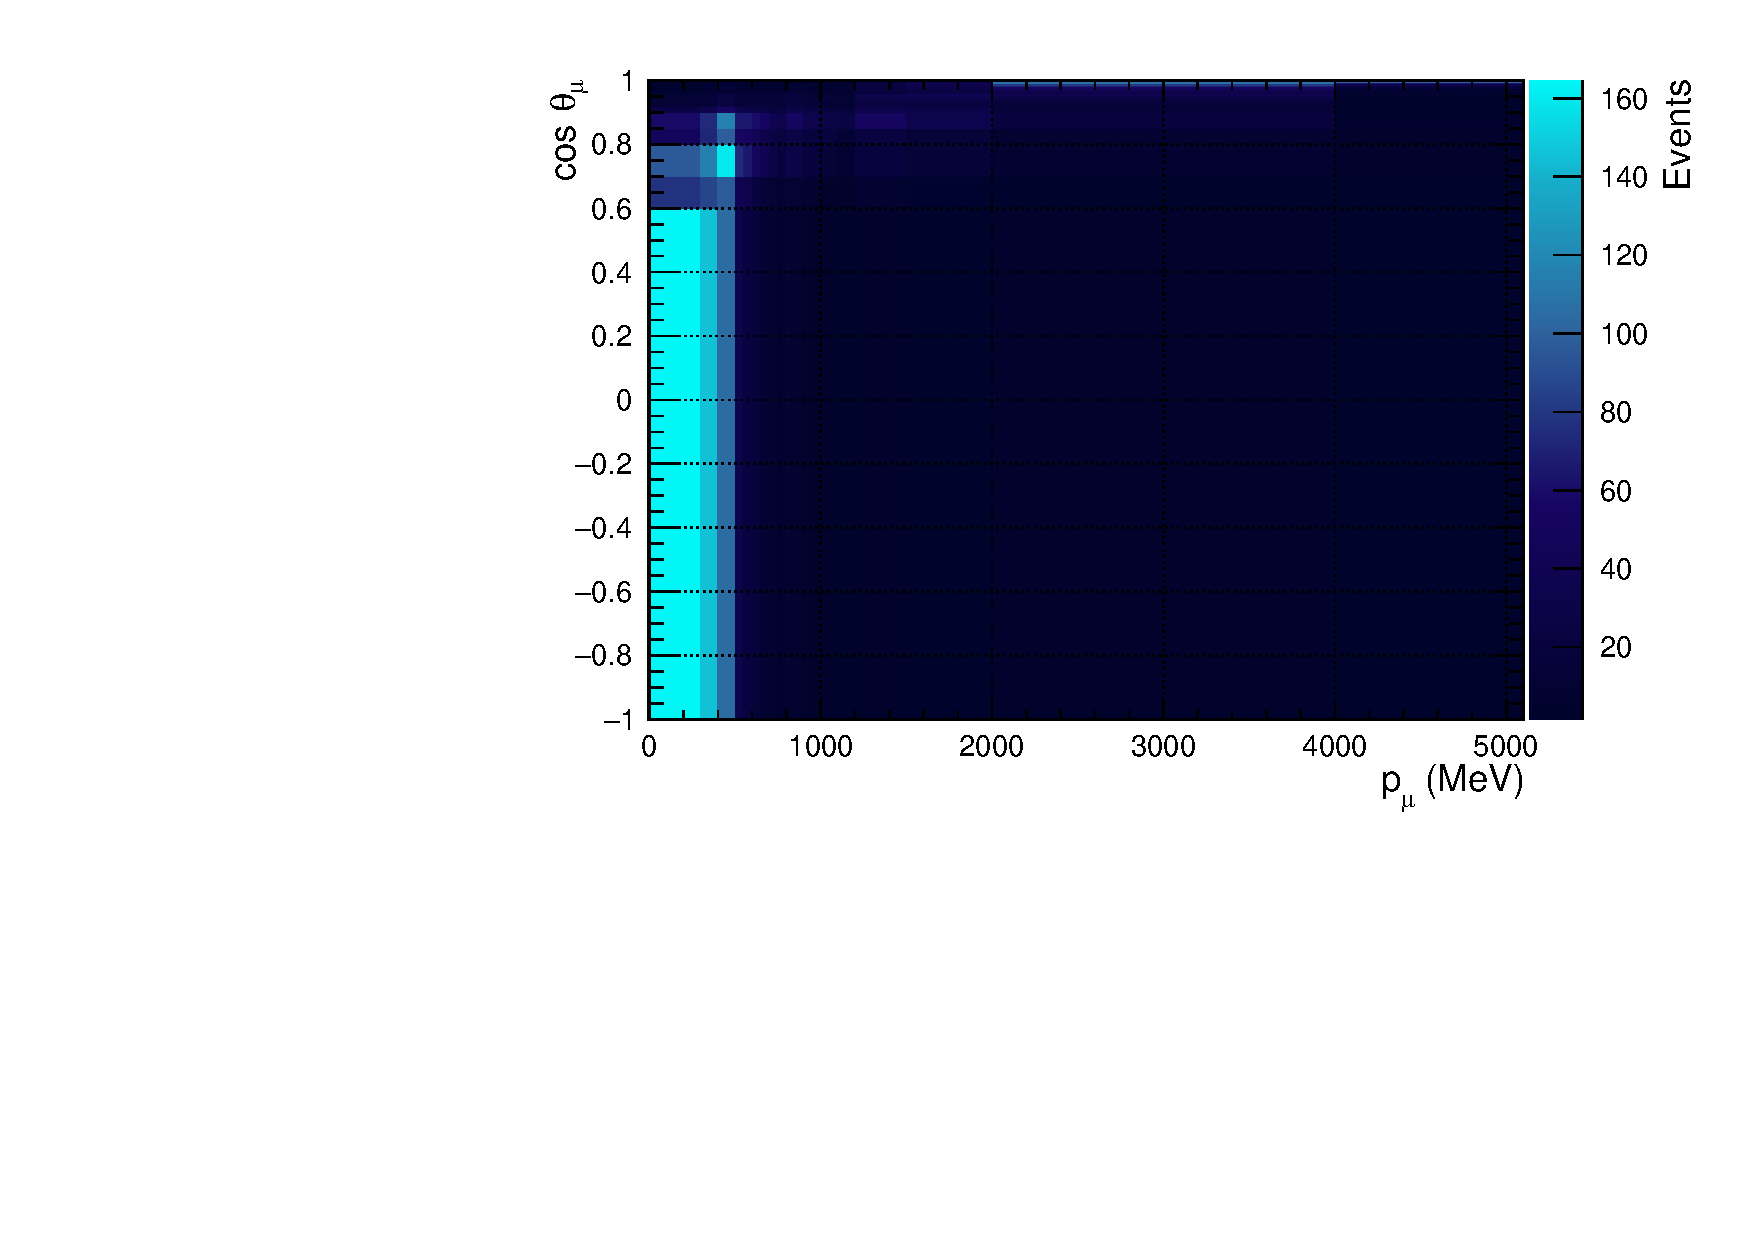
\includegraphics[width=0.95\linewidth]{figs/NomMC_MC_FGD2_anti-numuCC_0pi}
  \caption{FGD2 RHC $\bar{\nu_{\mu}}$ 0$\pi$}
  \label{fig:2d_FGD2_anti-numuCC_0pi}
\end{subfigure}
\begin{subfigure}{.32\textwidth}
  \centering
  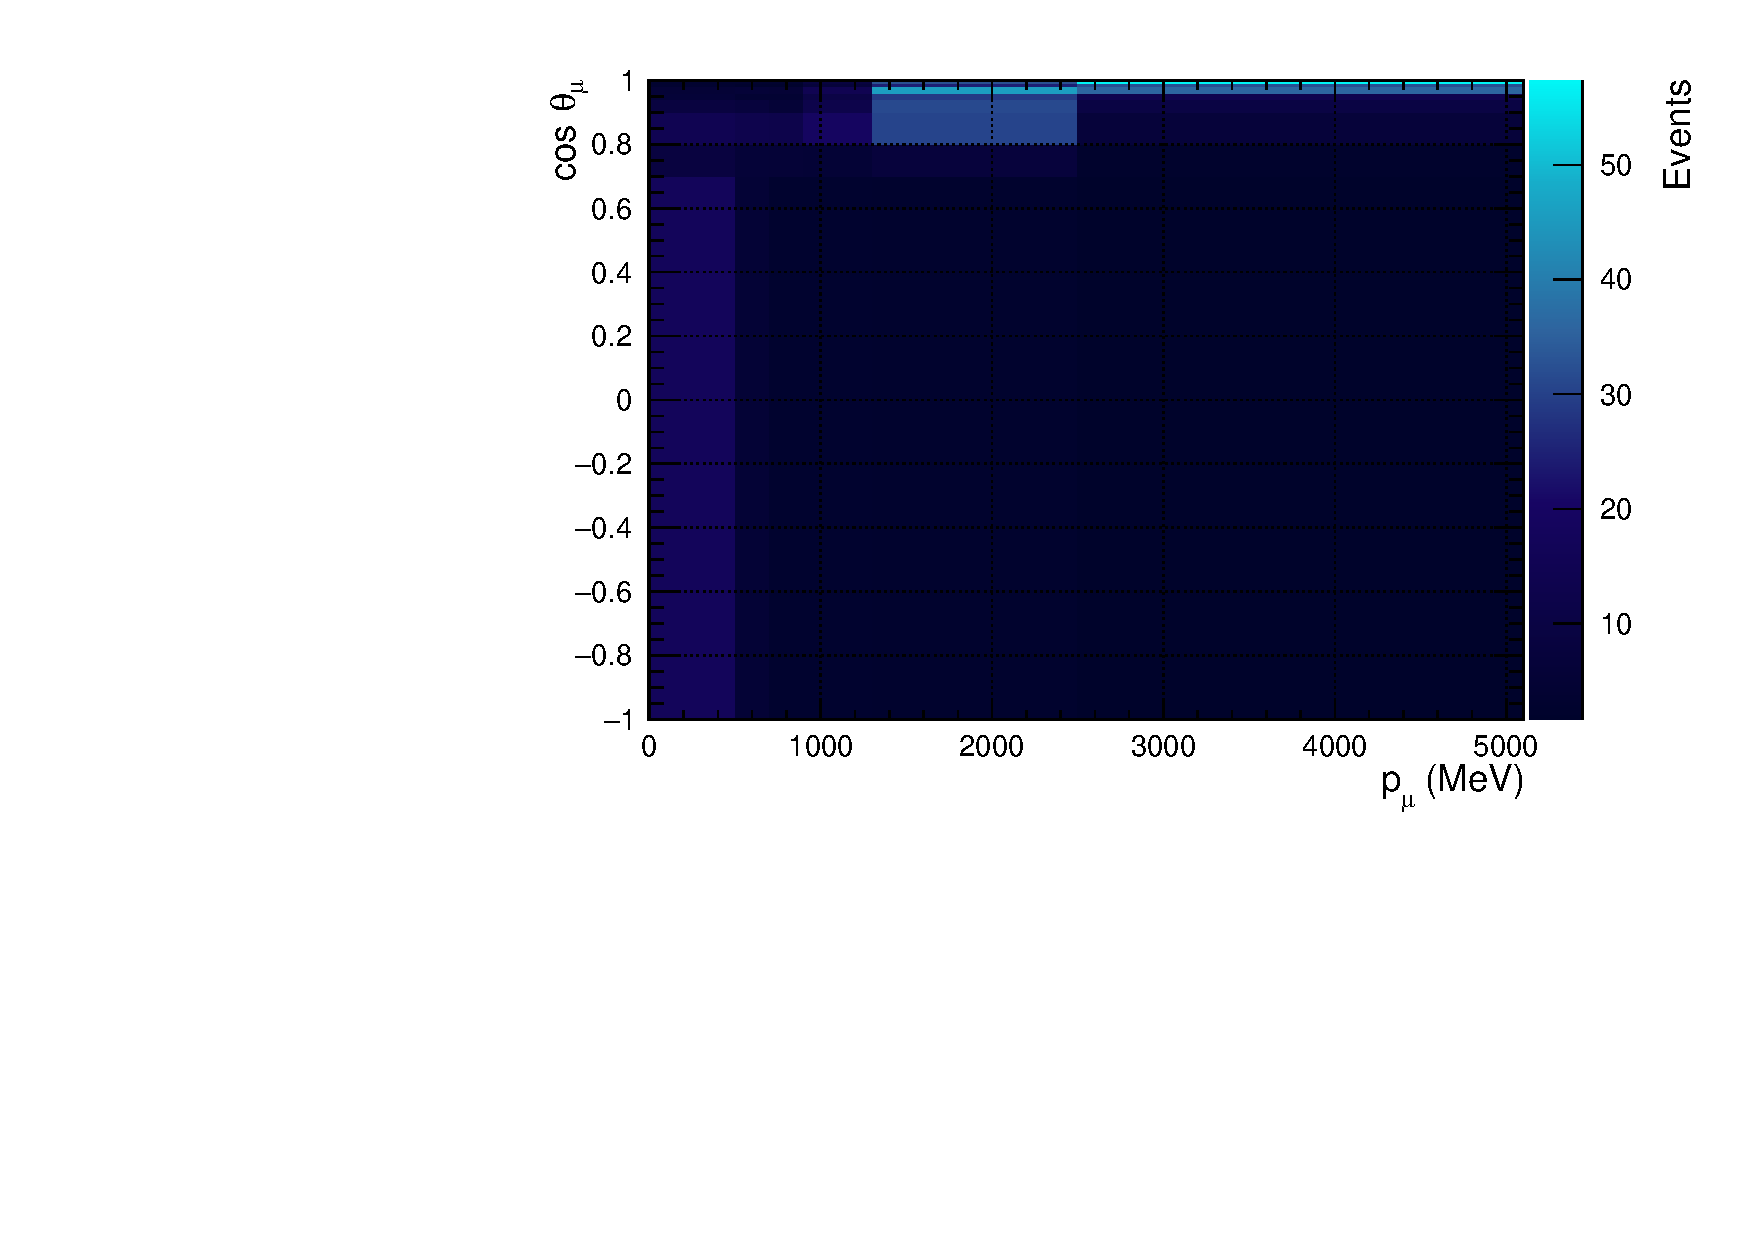
\includegraphics[width=0.95\linewidth]{figs/NomMC_MC_FGD2_anti-numuCC_1pi}
  \caption{FGD2 RHC $\bar{\nu_{\mu}}$ 1$\pi$}
  \label{fig:2d_FGD2_anti-numuCC_1pi}
\end{subfigure}
\begin{subfigure}{.32\textwidth}
  \centering
  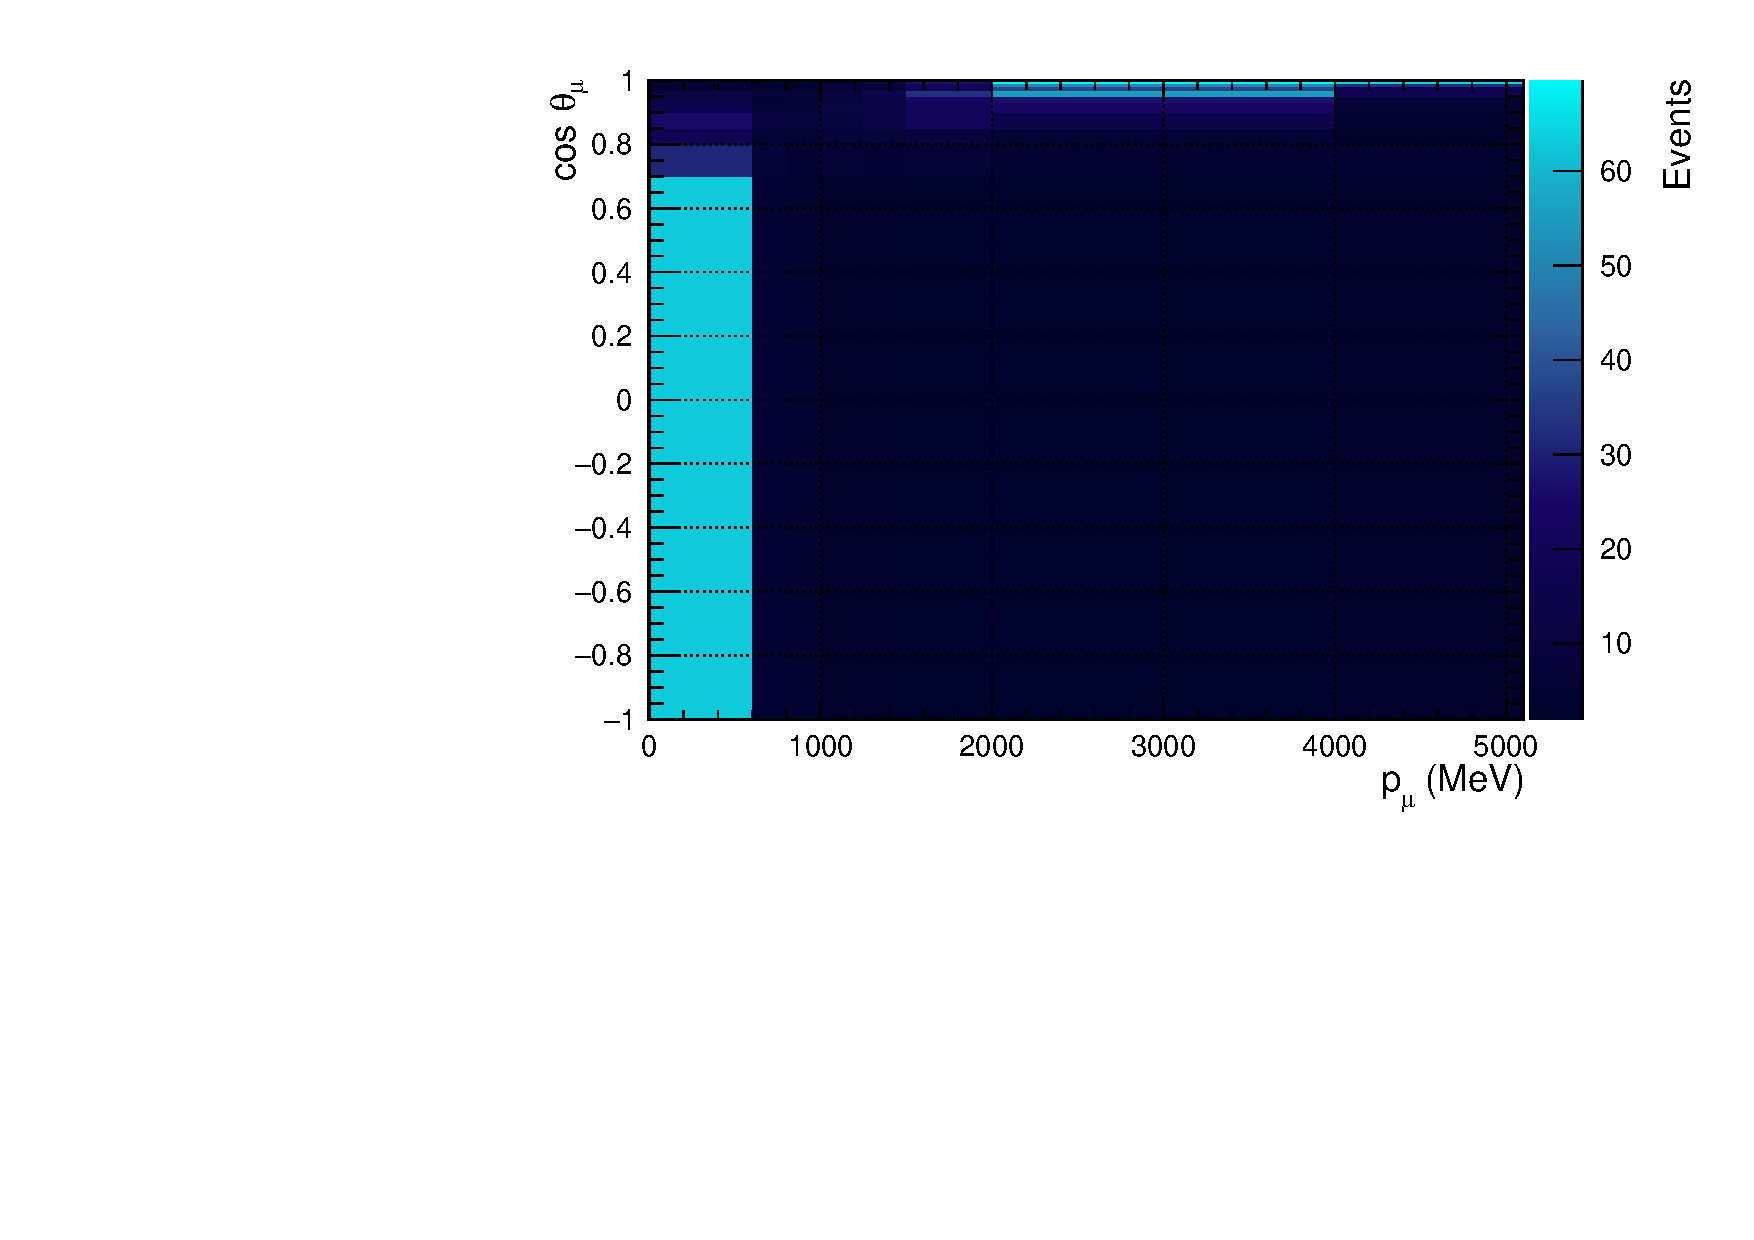
\includegraphics[width=0.95\linewidth]{figs/NomMC_MC_FGD2_anti-numuCC_other}
  \caption{FGD2 RHC $\bar{\nu_{\mu}}$ Other}
  \label{fig:2d_FGD2_anti-numuCC_other}
\end{subfigure}
\begin{subfigure}{.32\textwidth}
  \centering
  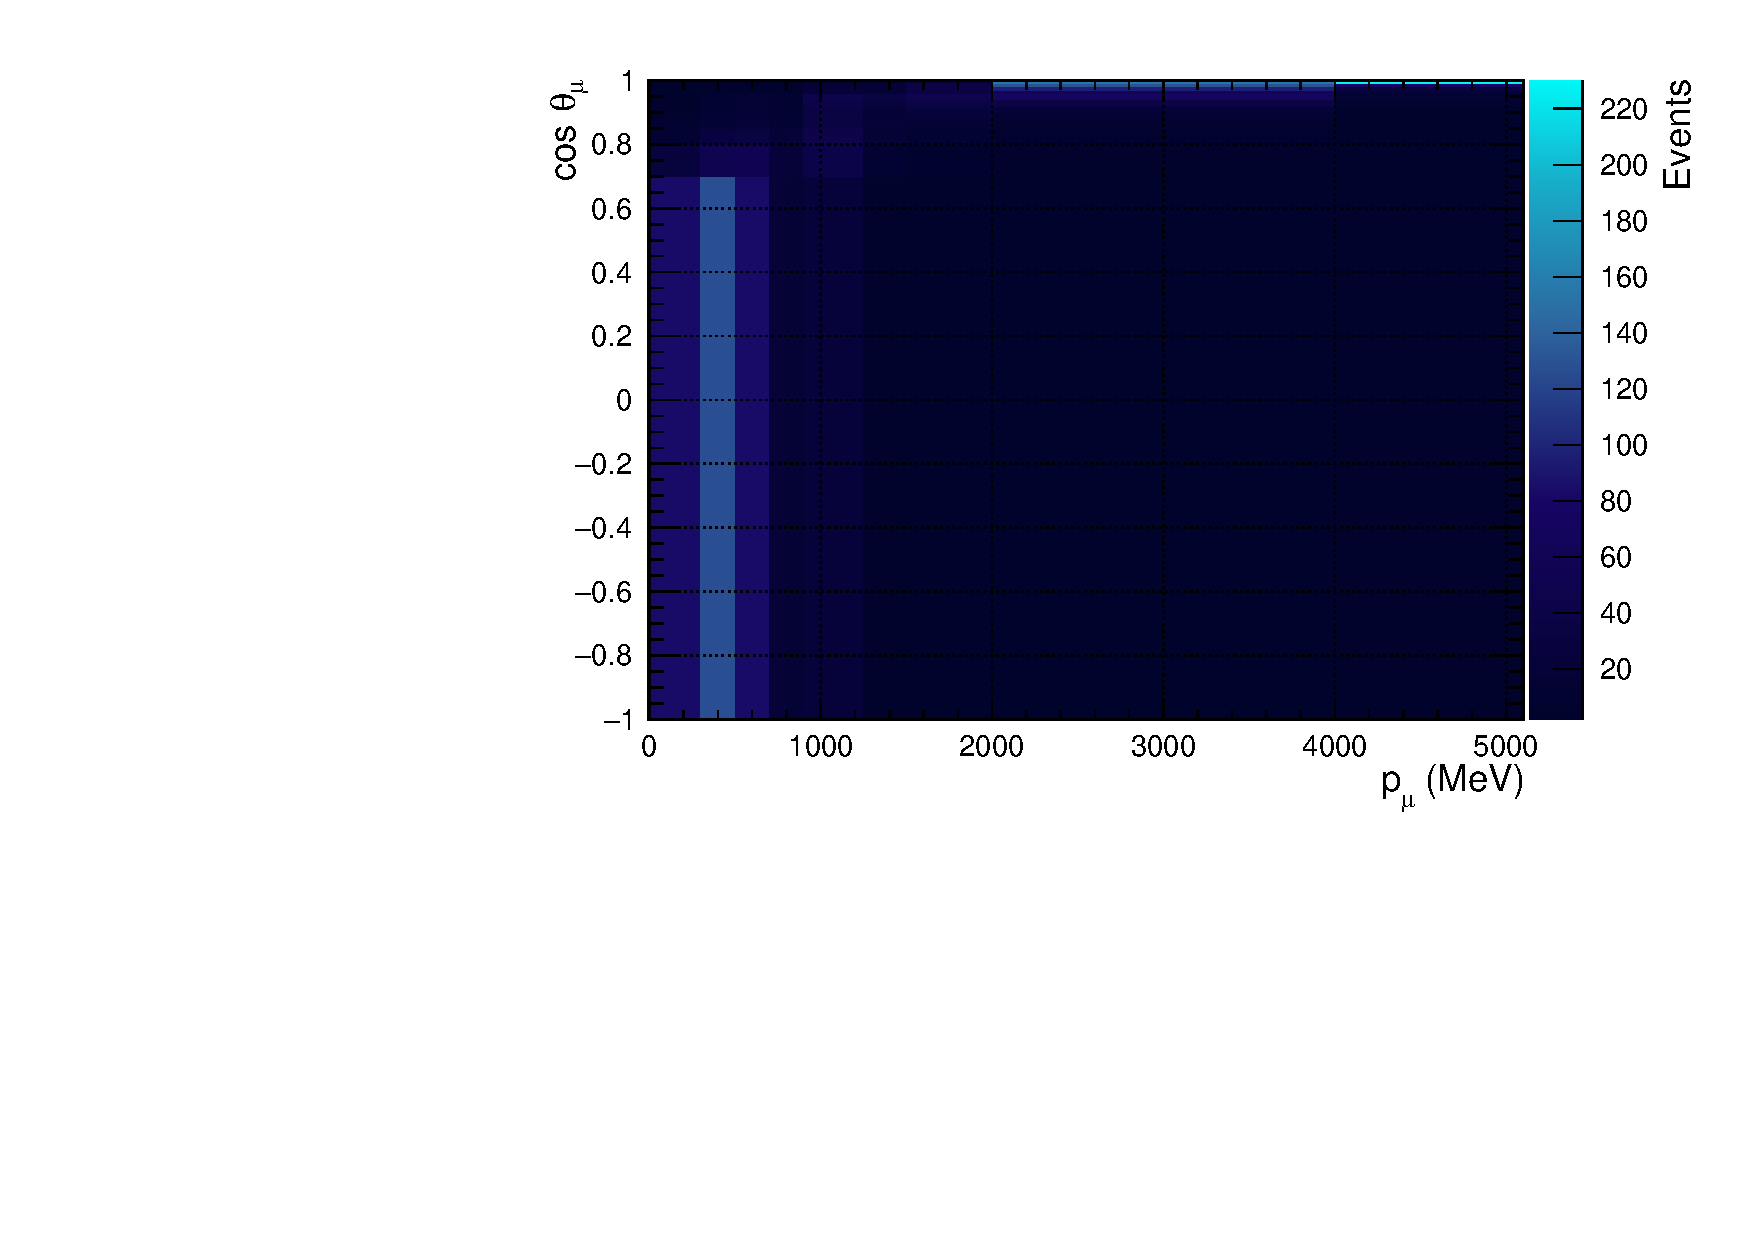
\includegraphics[width=0.95\linewidth]{figs/NomMC_MC_FGD1_NuMuBkg_CC0pi_in_AntiNu_Mode}
  \caption{FGD1 RHC $\nu_{\mu}$ 0$\pi$}
  \label{fig:2d_FGD1_NuMuBkg_CC0pi_in_AntiNu_Mode}
\end{subfigure}
\begin{subfigure}{.32\textwidth}
  \centering
  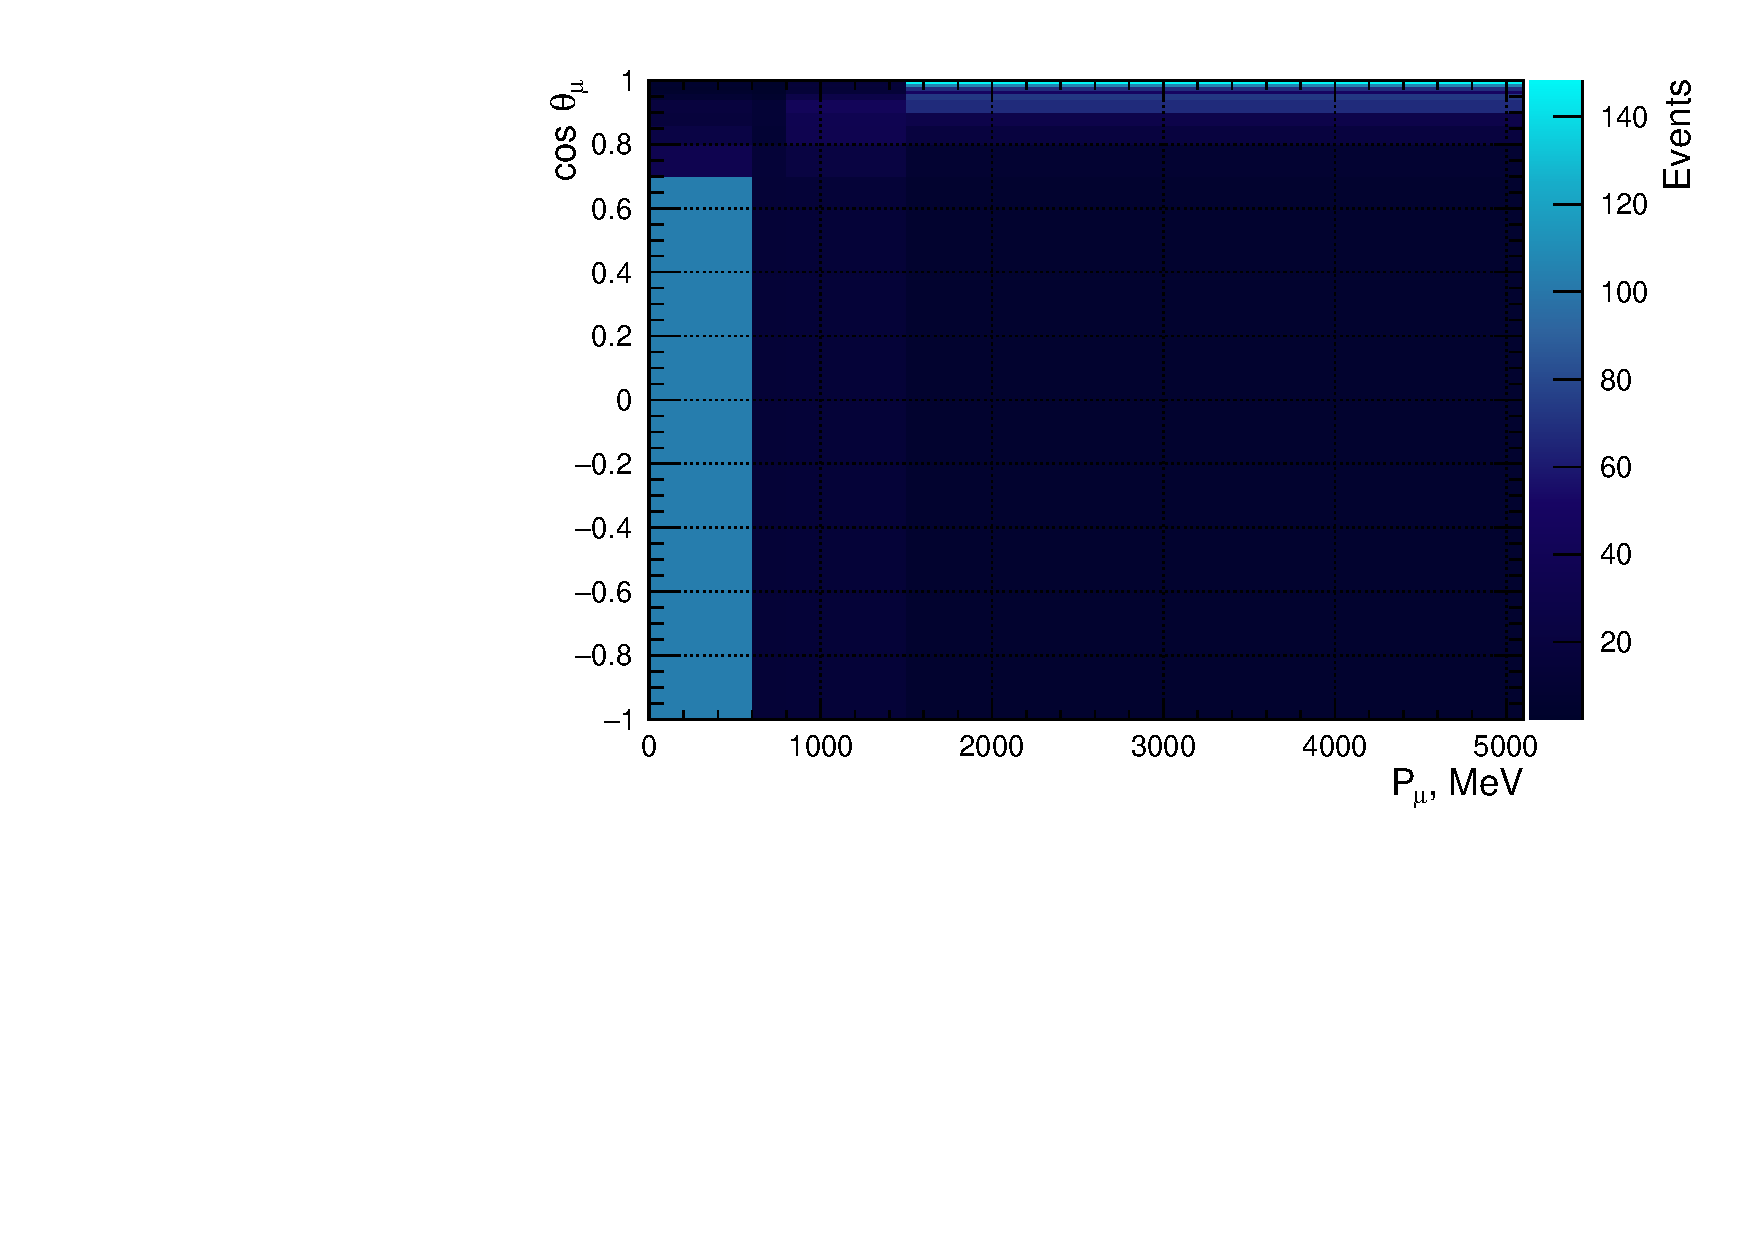
\includegraphics[width=0.95\linewidth]{figs/NomMC_MC_FGD1_NuMuBkg_CC1pi_in_AntiNu_Mode}
  \caption{FGD1 RHC $\nu_{\mu}$ 1$\pi$}
  \label{fig:2d_FGD1_NuMuBkg_CC1pi_in_AntiNu_Mode}
\end{subfigure}
\begin{subfigure}{.32\textwidth}
  \centering
  \includegraphics[width=0.95\linewidth]{figs/NomMC_MC_FGD1_NuMuBkg_CCOther_in_AntiNu_Mode}
  \caption{FGD1 RHC $\nu_{\mu}$ Other}
  \label{fig:2d_FGD1_NuMuBkg_CCOther_in_AntiNu_Mode}
\end{subfigure}
\begin{subfigure}{.32\textwidth}
  \centering
  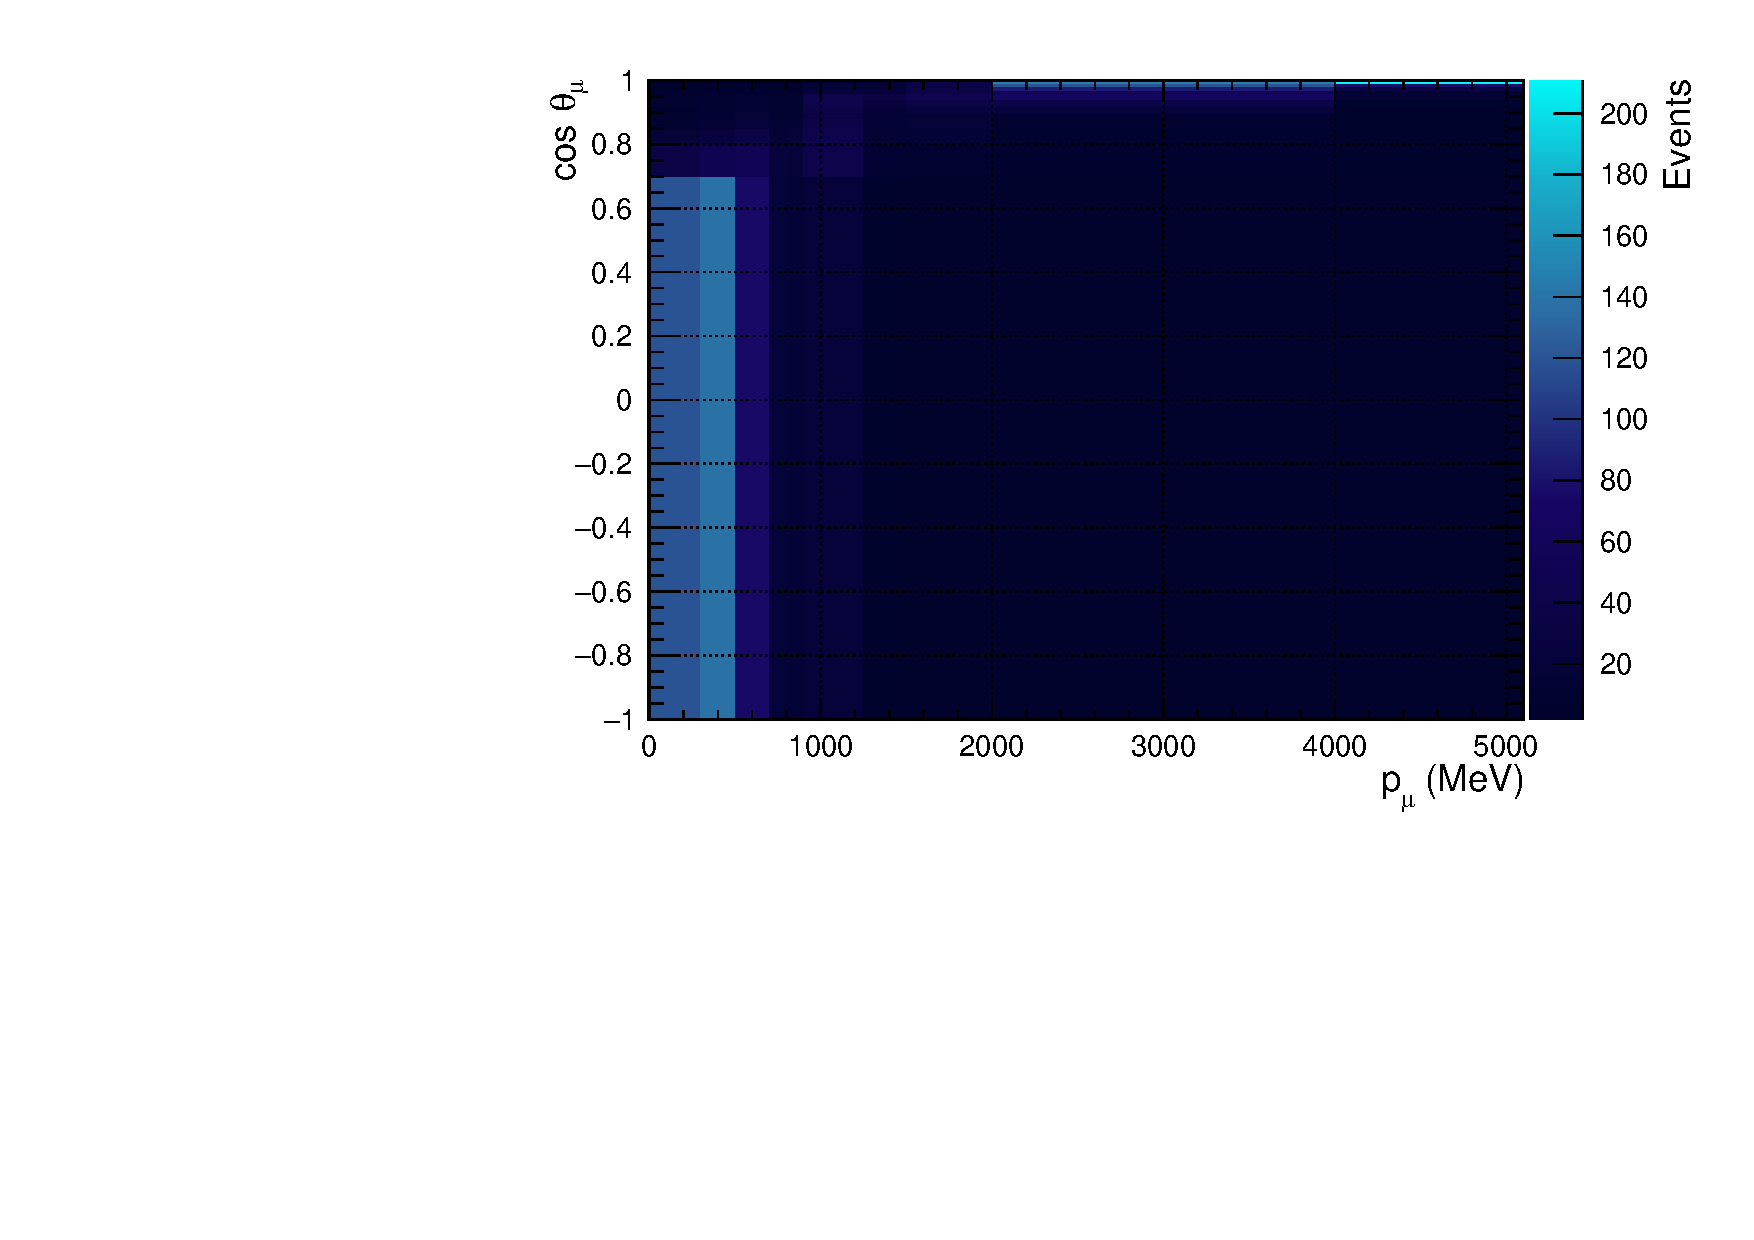
\includegraphics[width=0.95\linewidth]{figs/NomMC_MC_FGD2_NuMuBkg_CC0pi_in_AntiNu_Mode}
  \caption{FGD2 RHC $\nu_{\mu}$ 0$\pi$}
  \label{fig:2d_FGD2_NuMuBkg_CC0pi_in_AntiNu_Mode}
\end{subfigure}
\begin{subfigure}{.32\textwidth}
  \centering
  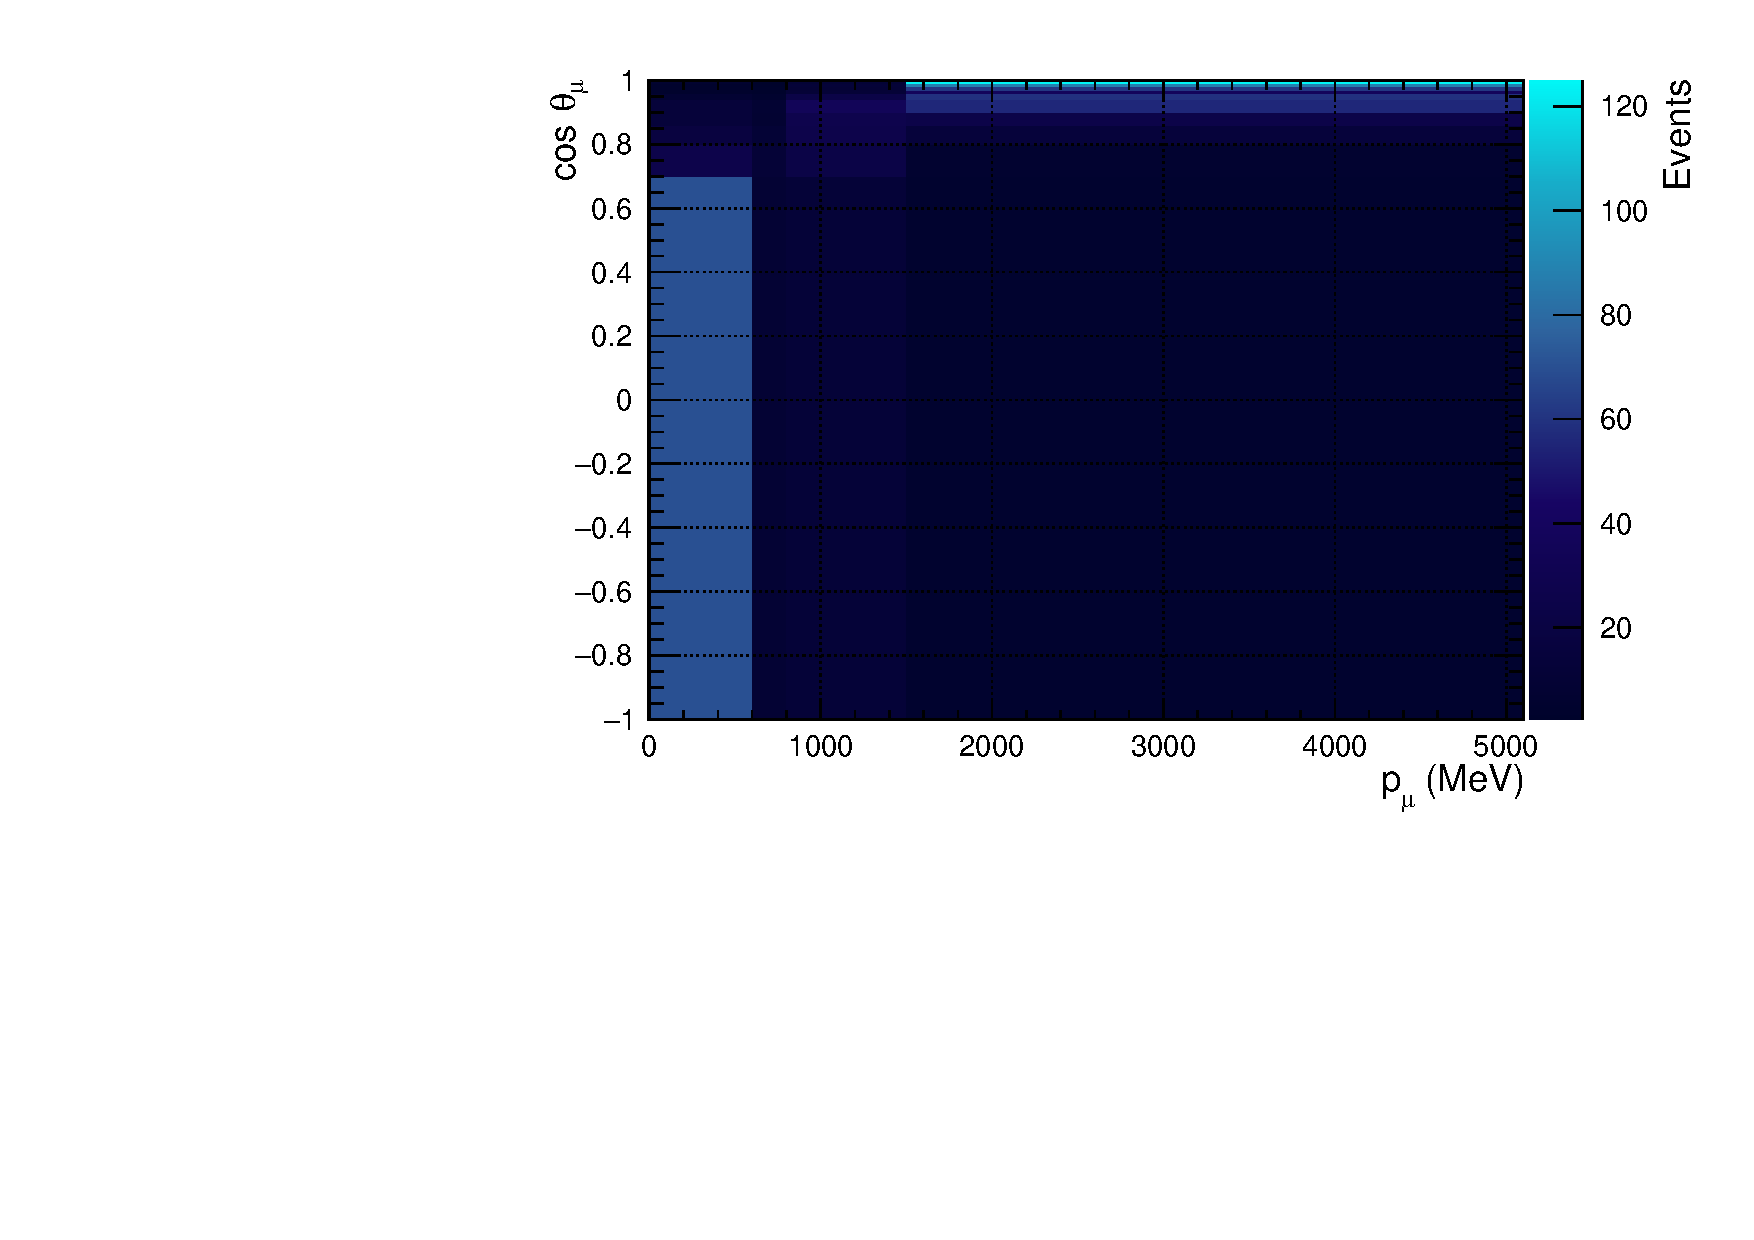
\includegraphics[width=0.95\linewidth]{figs/NomMC_MC_FGD2_NuMuBkg_CC1pi_in_AntiNu_Mode}
  \caption{FGD2 RHC $\nu_{\mu}$ 1$\pi$}
  \label{fig:2d_FGD2_NuMuBkg_CC1pi_in_AntiNu_Mode}
\end{subfigure}
\begin{subfigure}{.32\textwidth}
  \centering
  \includegraphics[width=0.95\linewidth]{figs/NomMC_MC_FGD2_NuMuBkg_CCOther_in_AntiNu_Mode}
  \caption{FGD2 RHC $\nu_{\mu}$ Other}
  \label{fig:2d_FGD2_NuMuBkg_CCOther_in_AntiNu_Mode}
\end{subfigure}
\caption{$p_{\mu}$-cos $\theta_{\mu}$ distributions for the nominal MC.}
\label{fig:2dnom}
\end{figure}

The projection of these distributions onto the $p_{\mu}$ axis are shown in Figure \ref{fig:pstack}, along with the data and interaction mode breakdown.

The CC 0$\pi$ and CC Other samples show oscillatory behaviour in the ratio of data to MC at low momentum. The ratio is consistently $>1$, but is slightly increased at the peak momentum for FHC and RHC $\nu$, and decreased at the peak for RHC $\bar{\nu}$. The ratio for the CC 1$\pi$ samples is more flat in momentum, but shows a small oscillation $<1$ at low momentum for FHC $\nu$, and $>1$ for RHC $\nu$ and $\bar{\nu}$. The behaviour is similar across the FGDs.

The FHC $\nu$ and RHC $\bar{\nu}$ CC 0$\pi$ samples are dominated by the target interaction modes CCQE and 2p2h. However, for RHC $\nu$, there is a large contamination of CC 1$\pi$ events. The FHC $\nu$ and RHC $\bar{\nu}$ CC 1$\pi$ samples are dominated by the target interaction modes CC 1$\pi$, CC coherent, and CC mult-$\pi$. For RHC, $\nu$ the 1$\pi$ sample has a significant number of CC DIS events. The CC Other samples are populated by mainly the target interaction modes CC DIS, CC mult-$\pi$, and CC miscellaneous, but with a significant number CC $1\pi$ and CC coherent events for FHC $\nu$ and RHC $\bar{\nu}$.

\begin{figure}
\centering
\begin{subfigure}{.35\textwidth}
  \centering
  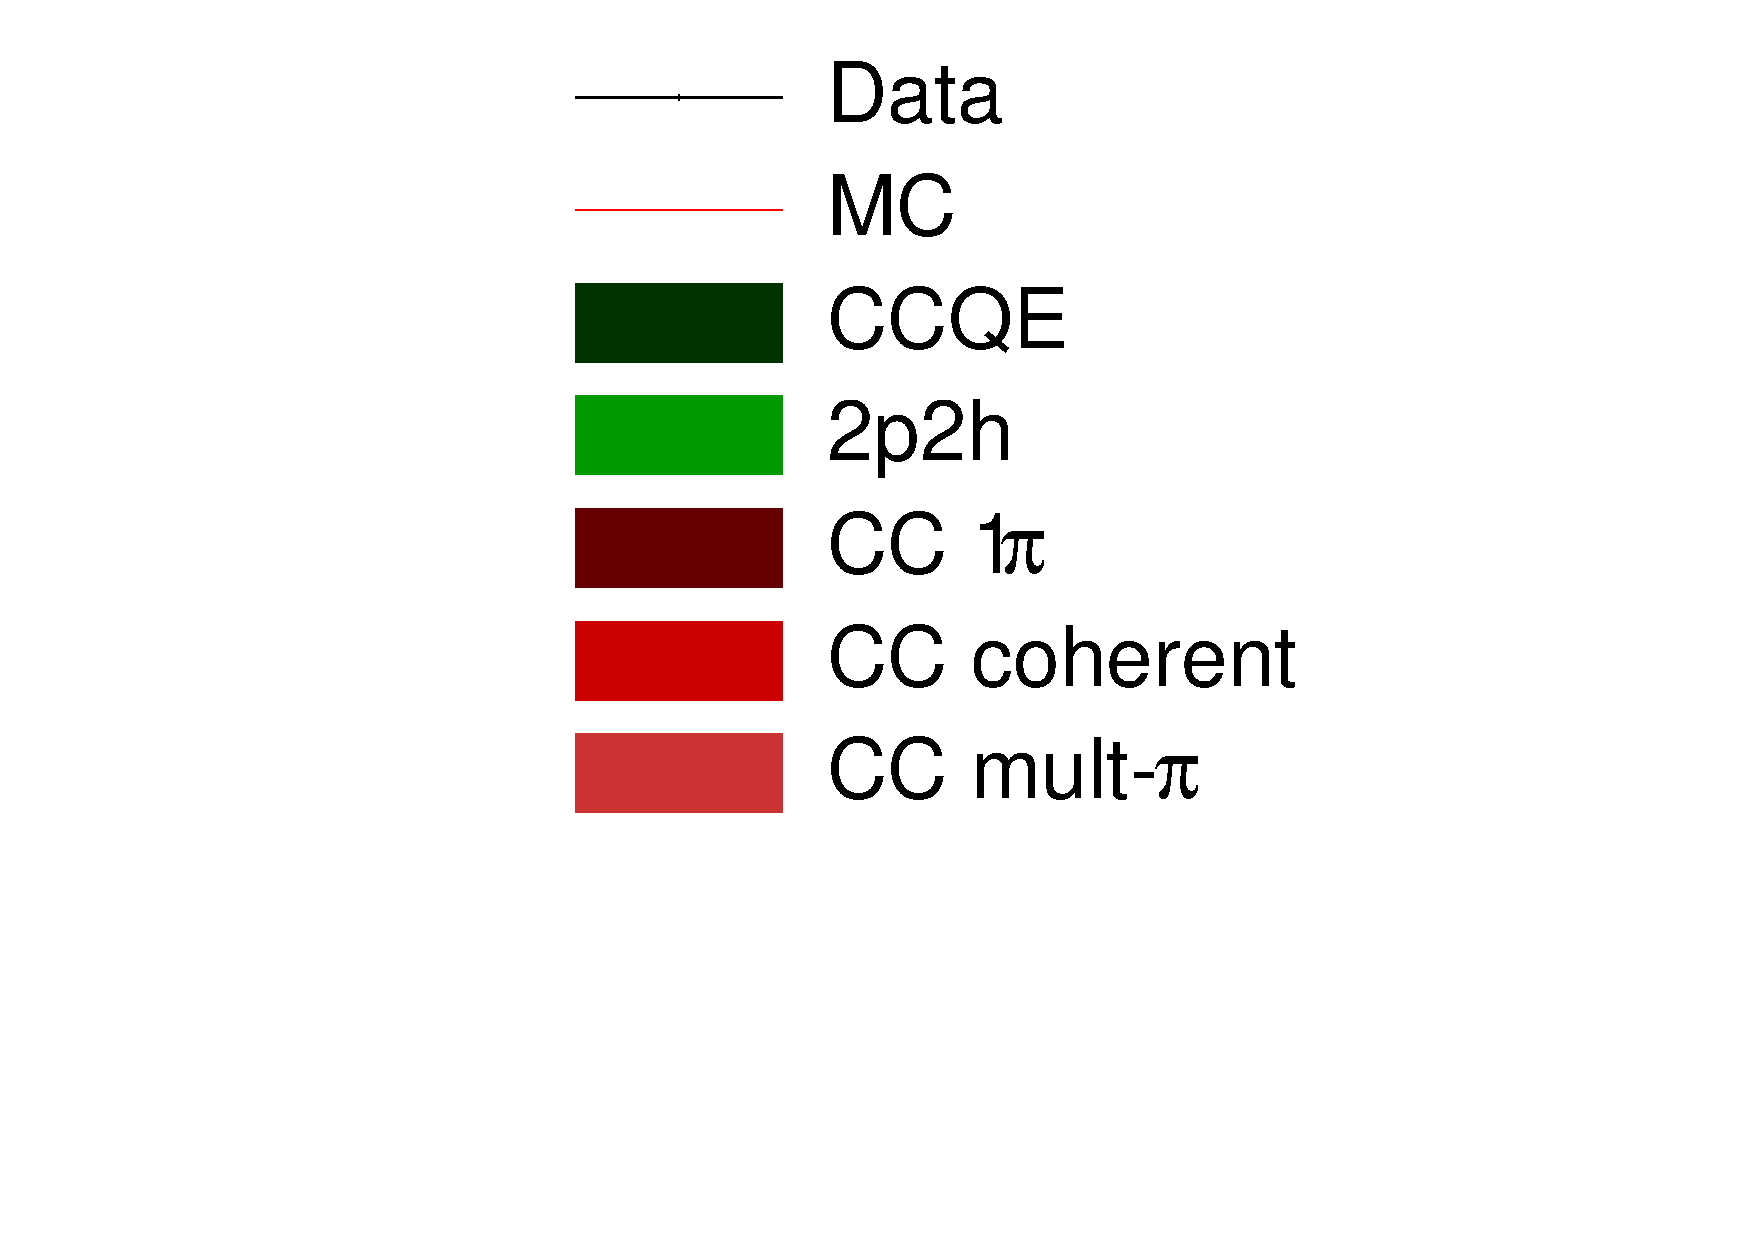
\includegraphics[width=0.7\linewidth]{figs/legend}
\end{subfigure}
\begin{subfigure}{.35\textwidth}
  \centering
  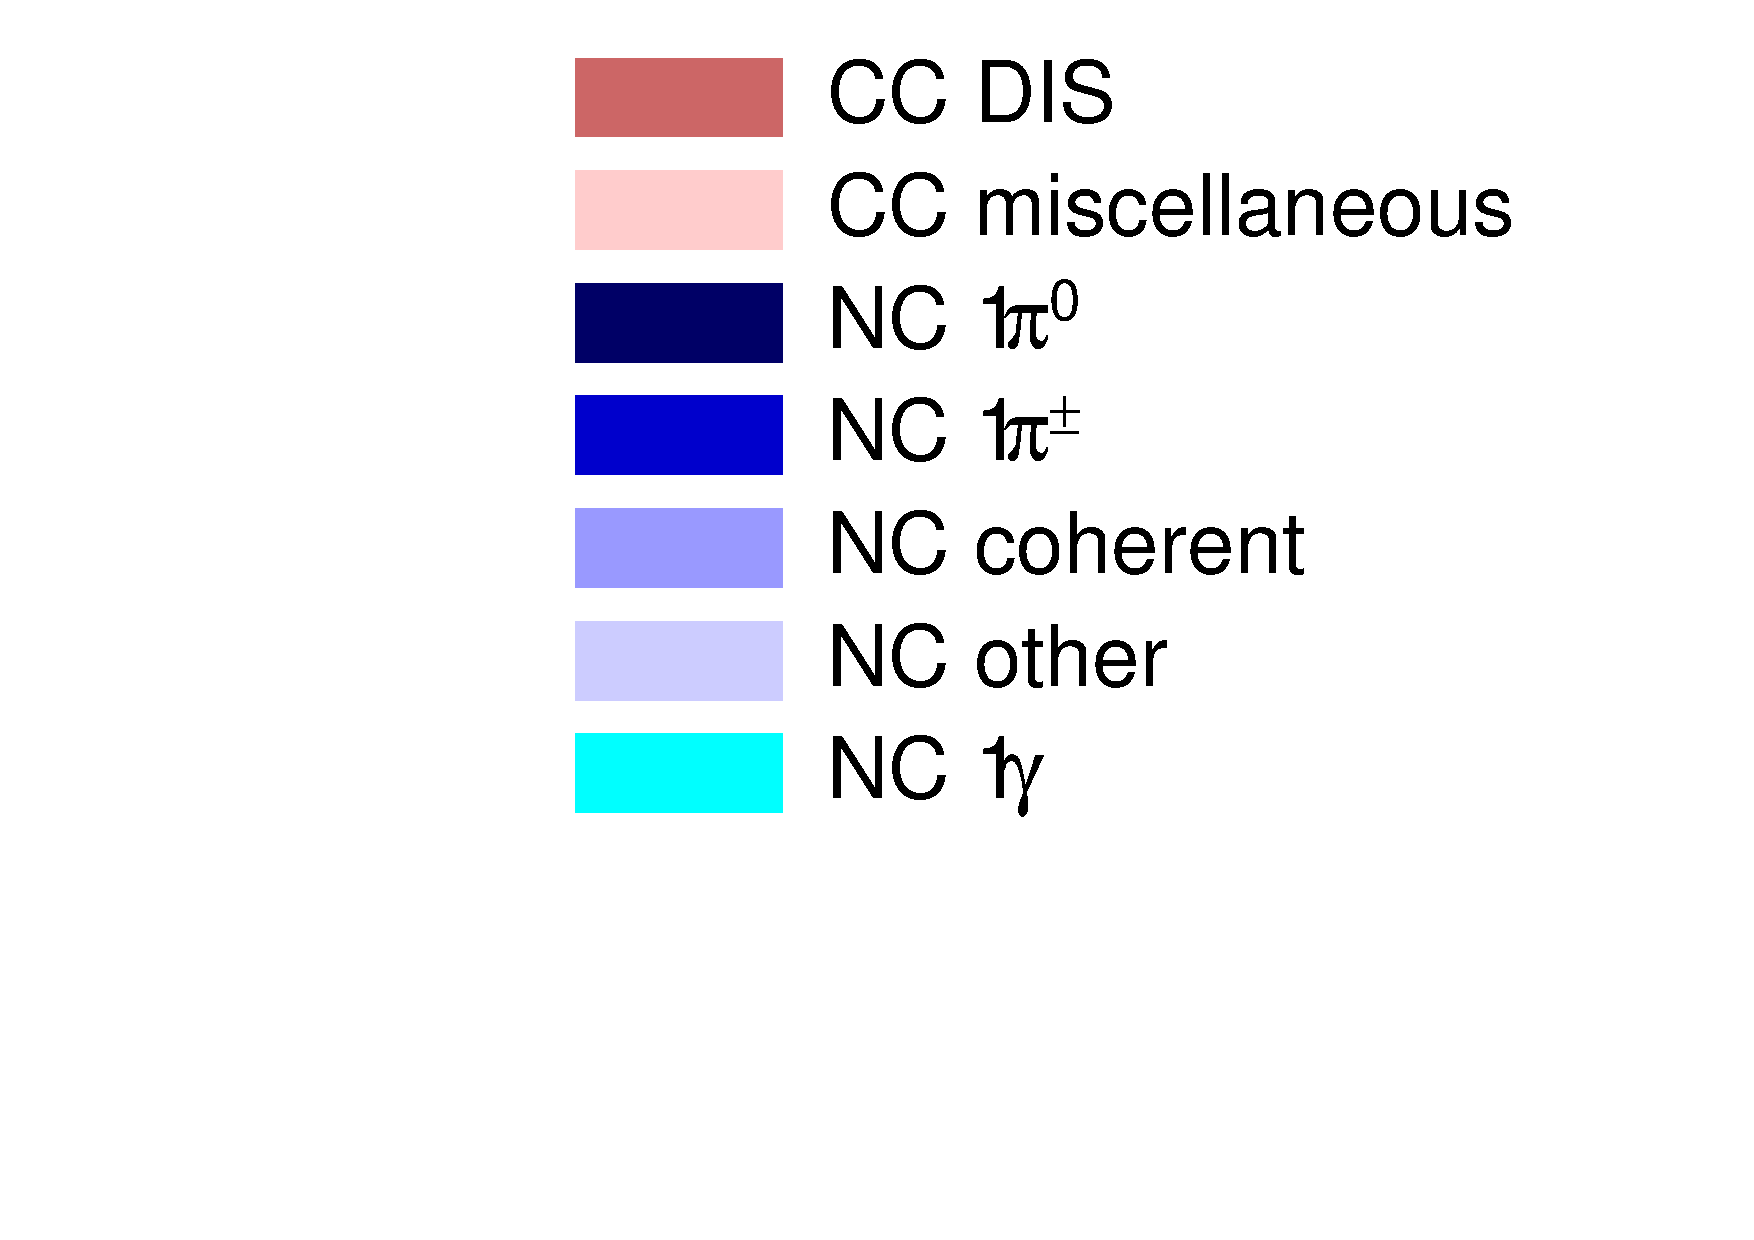
\includegraphics[width=0.7\linewidth]{figs/legend2}
\end{subfigure}
\begin{subfigure}{.32\textwidth}
  \centering
  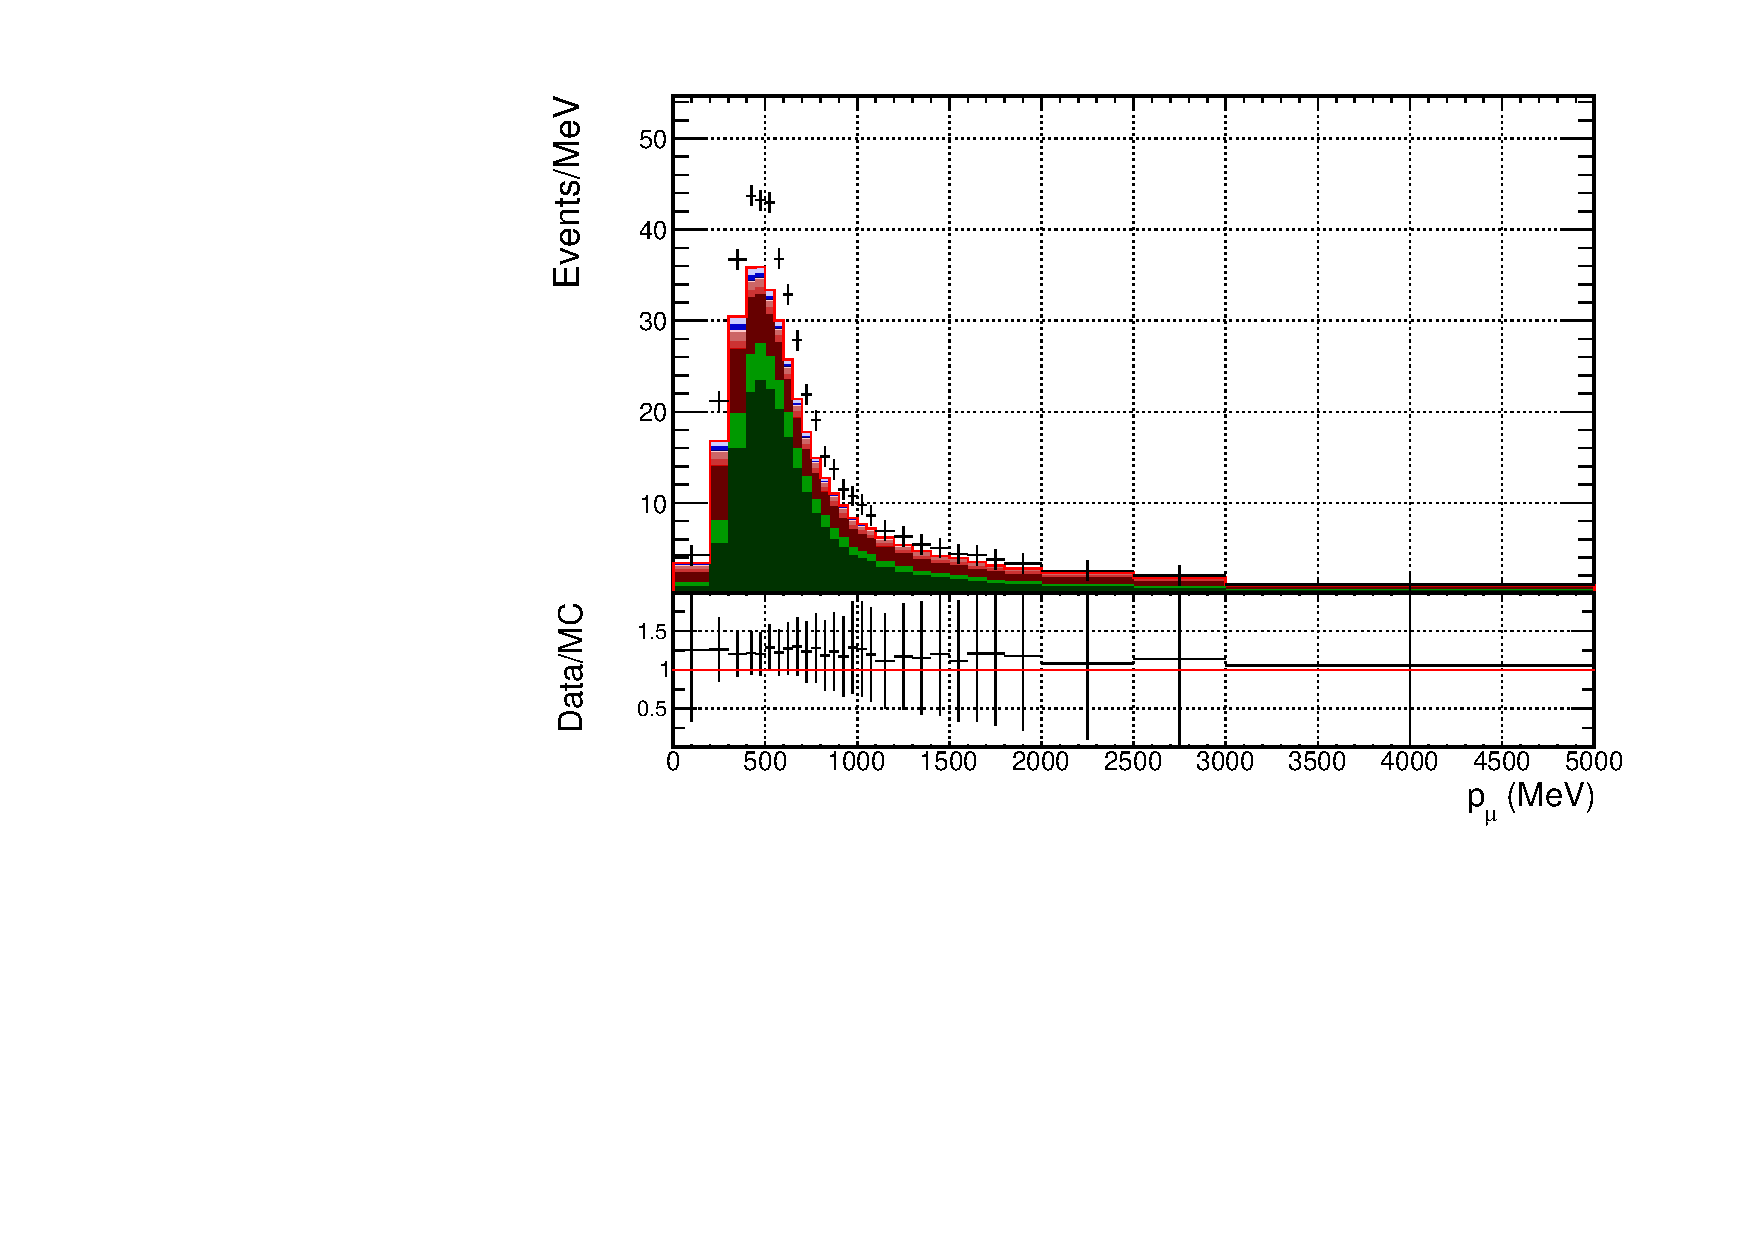
\includegraphics[width=0.95\linewidth]{figs/FGD1_numuCC_0pi_p}
  \caption{FGD1 FHC $\nu_{\mu}$ 0$\pi$}
  \label{fig:pstack_FGD1_numuCC_0pi}
\end{subfigure}
\begin{subfigure}{.32\textwidth}
  \centering
  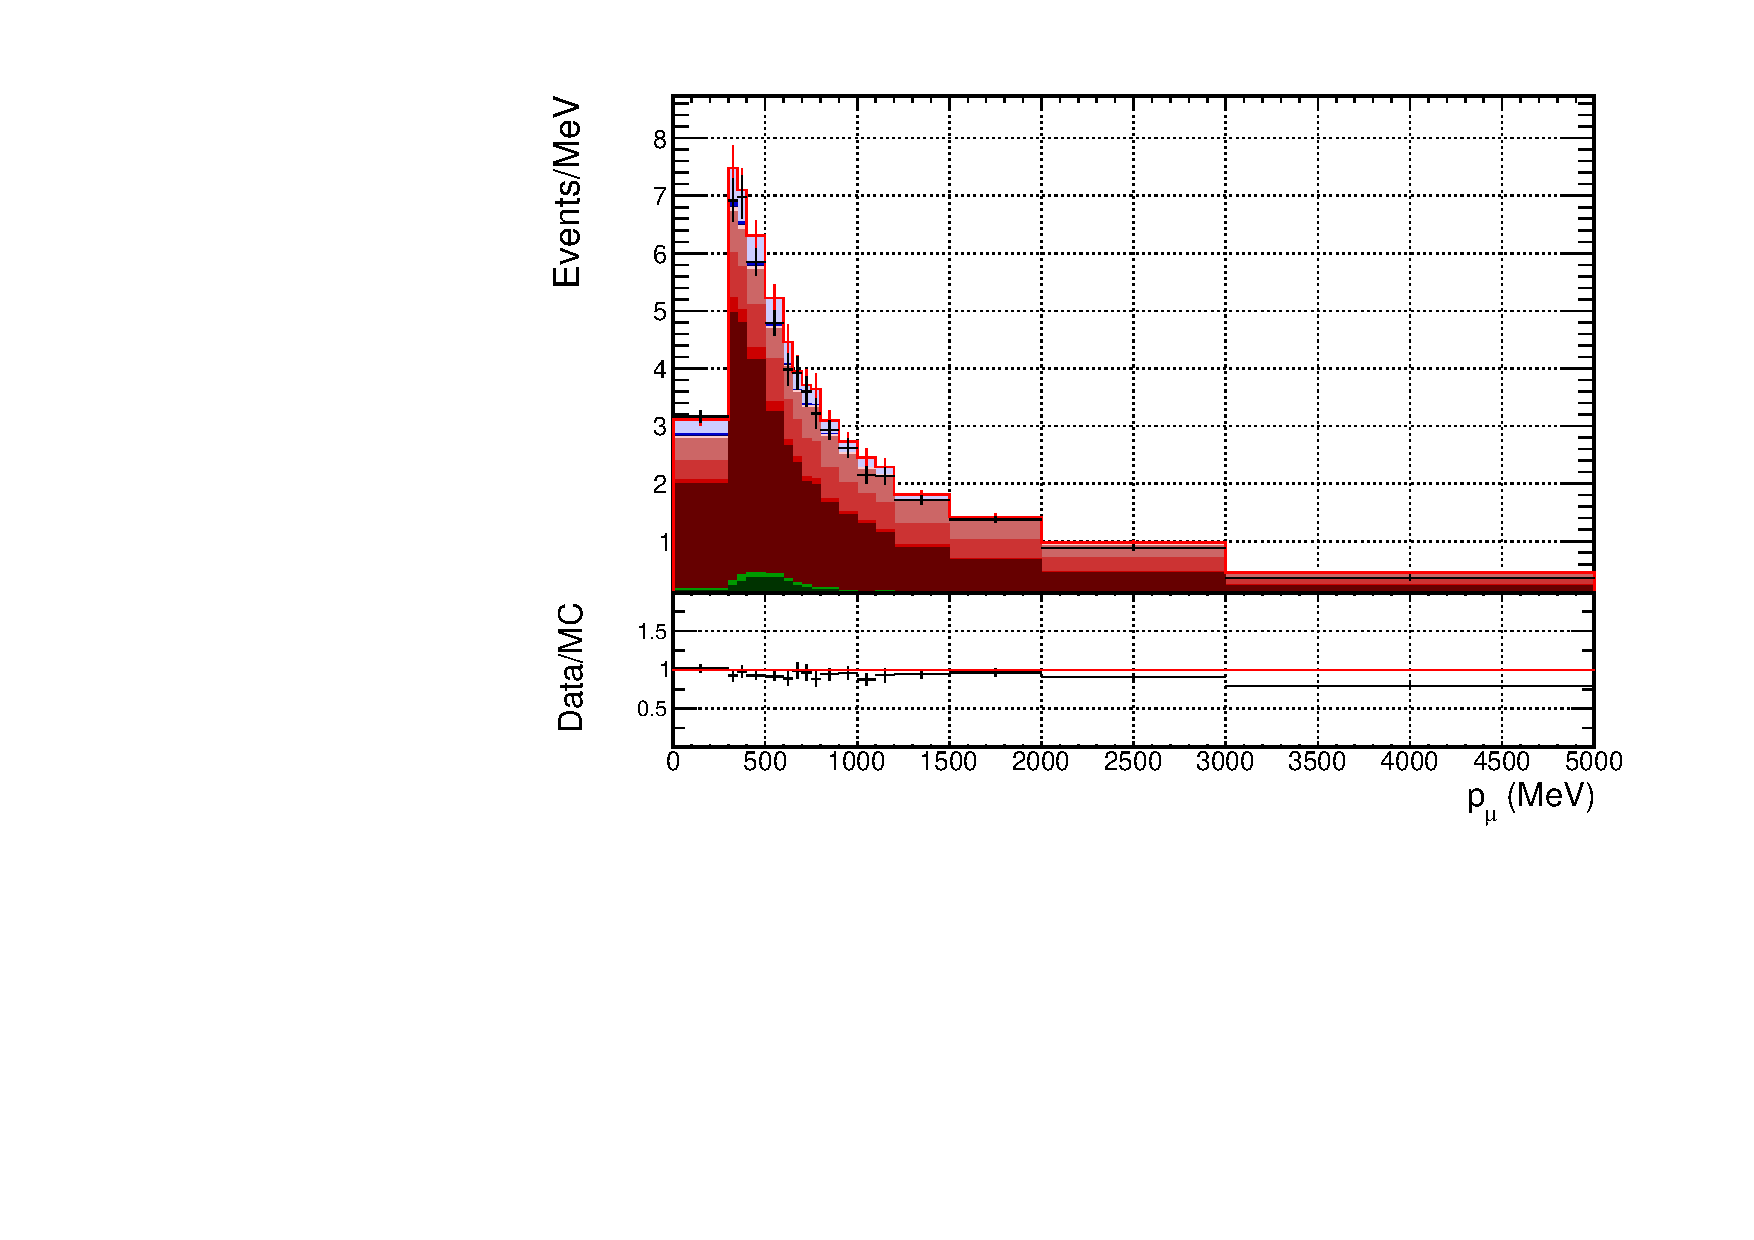
\includegraphics[width=0.95\linewidth]{figs/FGD1_numuCC_1pi_p}
  \caption{FGD1 FHC $\nu_{\mu}$ 1$\pi$}
  \label{fig:pstack_FGD1_numuCC_1pi}
\end{subfigure}
\begin{subfigure}{.32\textwidth}
  \centering
  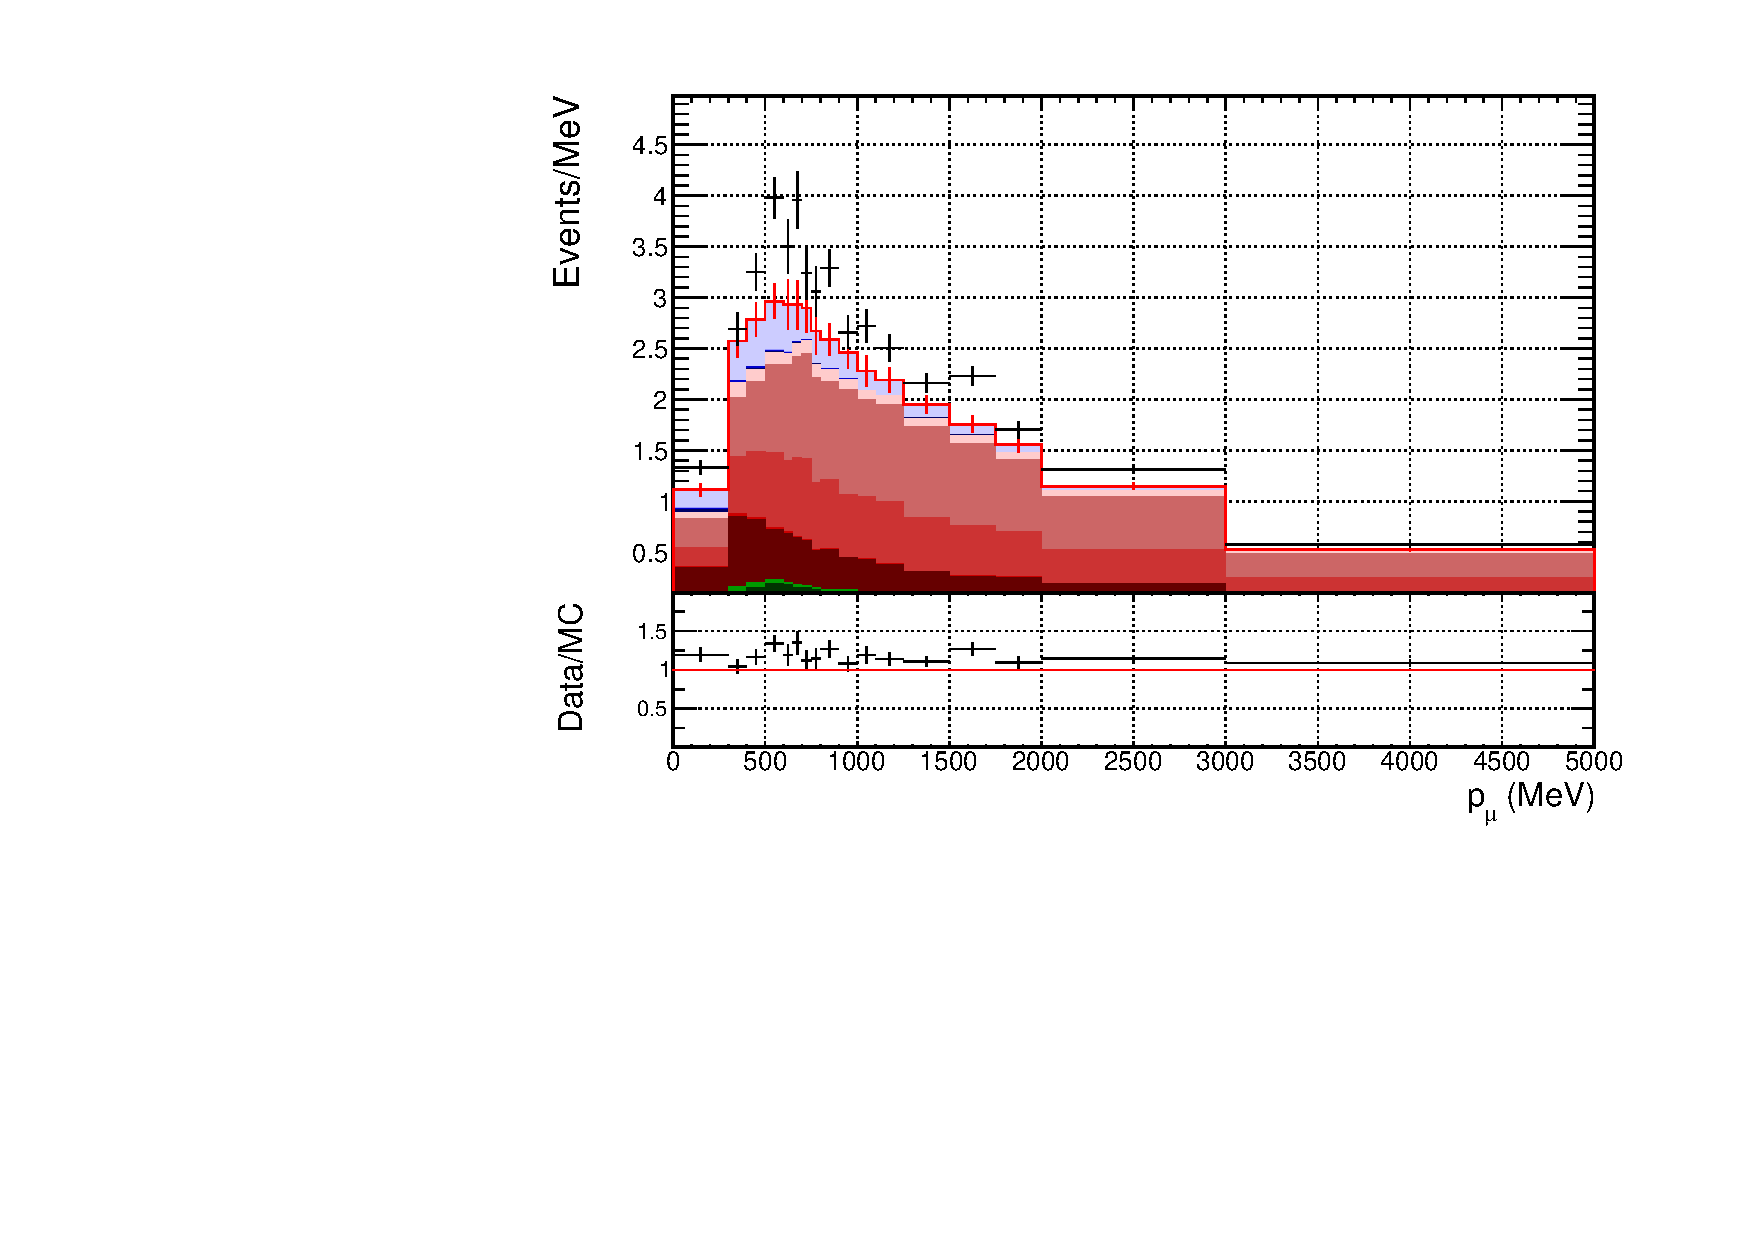
\includegraphics[width=0.95\linewidth]{figs/FGD1_numuCC_other_p}
  \caption{FGD1 FHC $\nu_{\mu}$ Other}
  \label{fig:pstack_FGD1_numuCC_other}
\end{subfigure}
\centering
\begin{subfigure}{.32\textwidth}
  \centering
  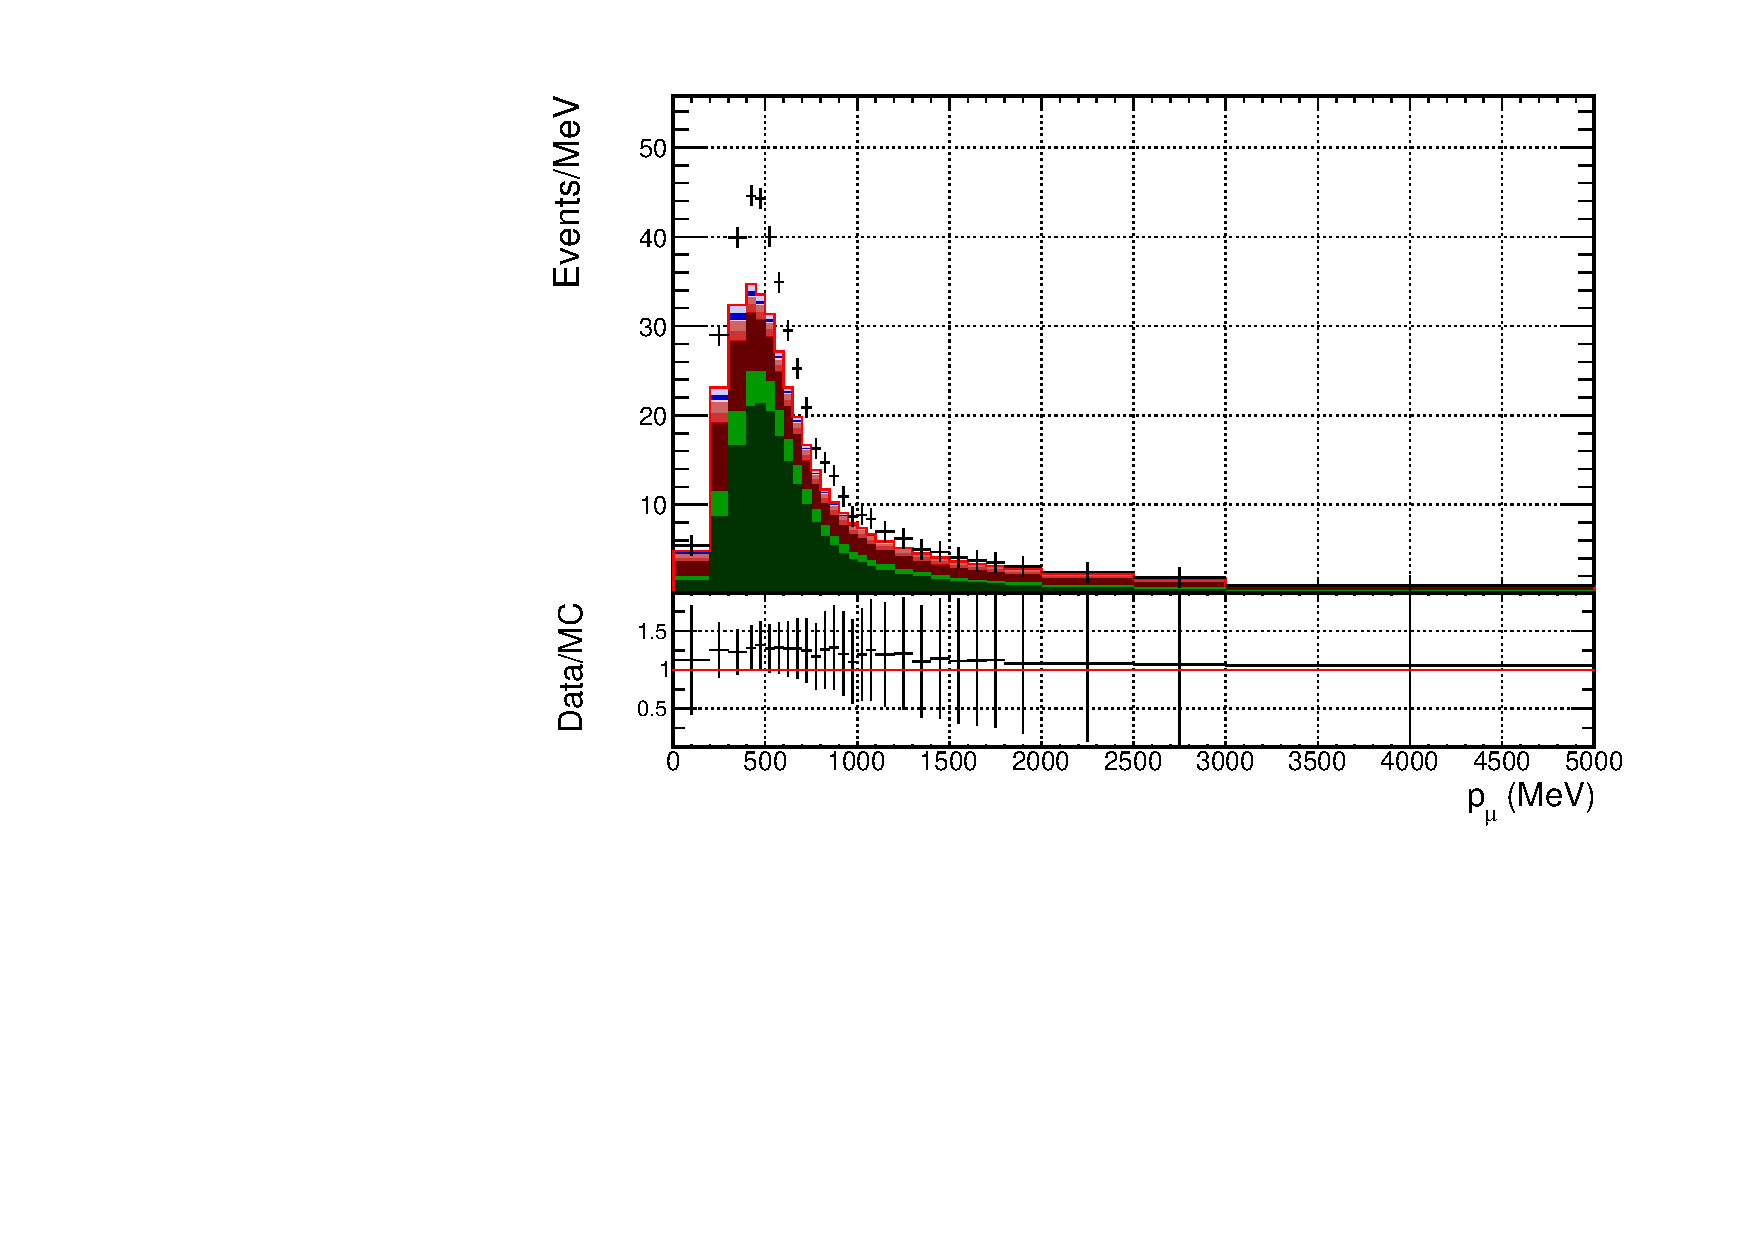
\includegraphics[width=0.95\linewidth]{figs/FGD2_numuCC_0pi_p}
  \caption{FGD2 FHC $\nu_{\mu}$ 0$\pi$}
  \label{fig:pstack_FGD2_numuCC_0pi}
\end{subfigure}
\begin{subfigure}{.32\textwidth}
  \centering
  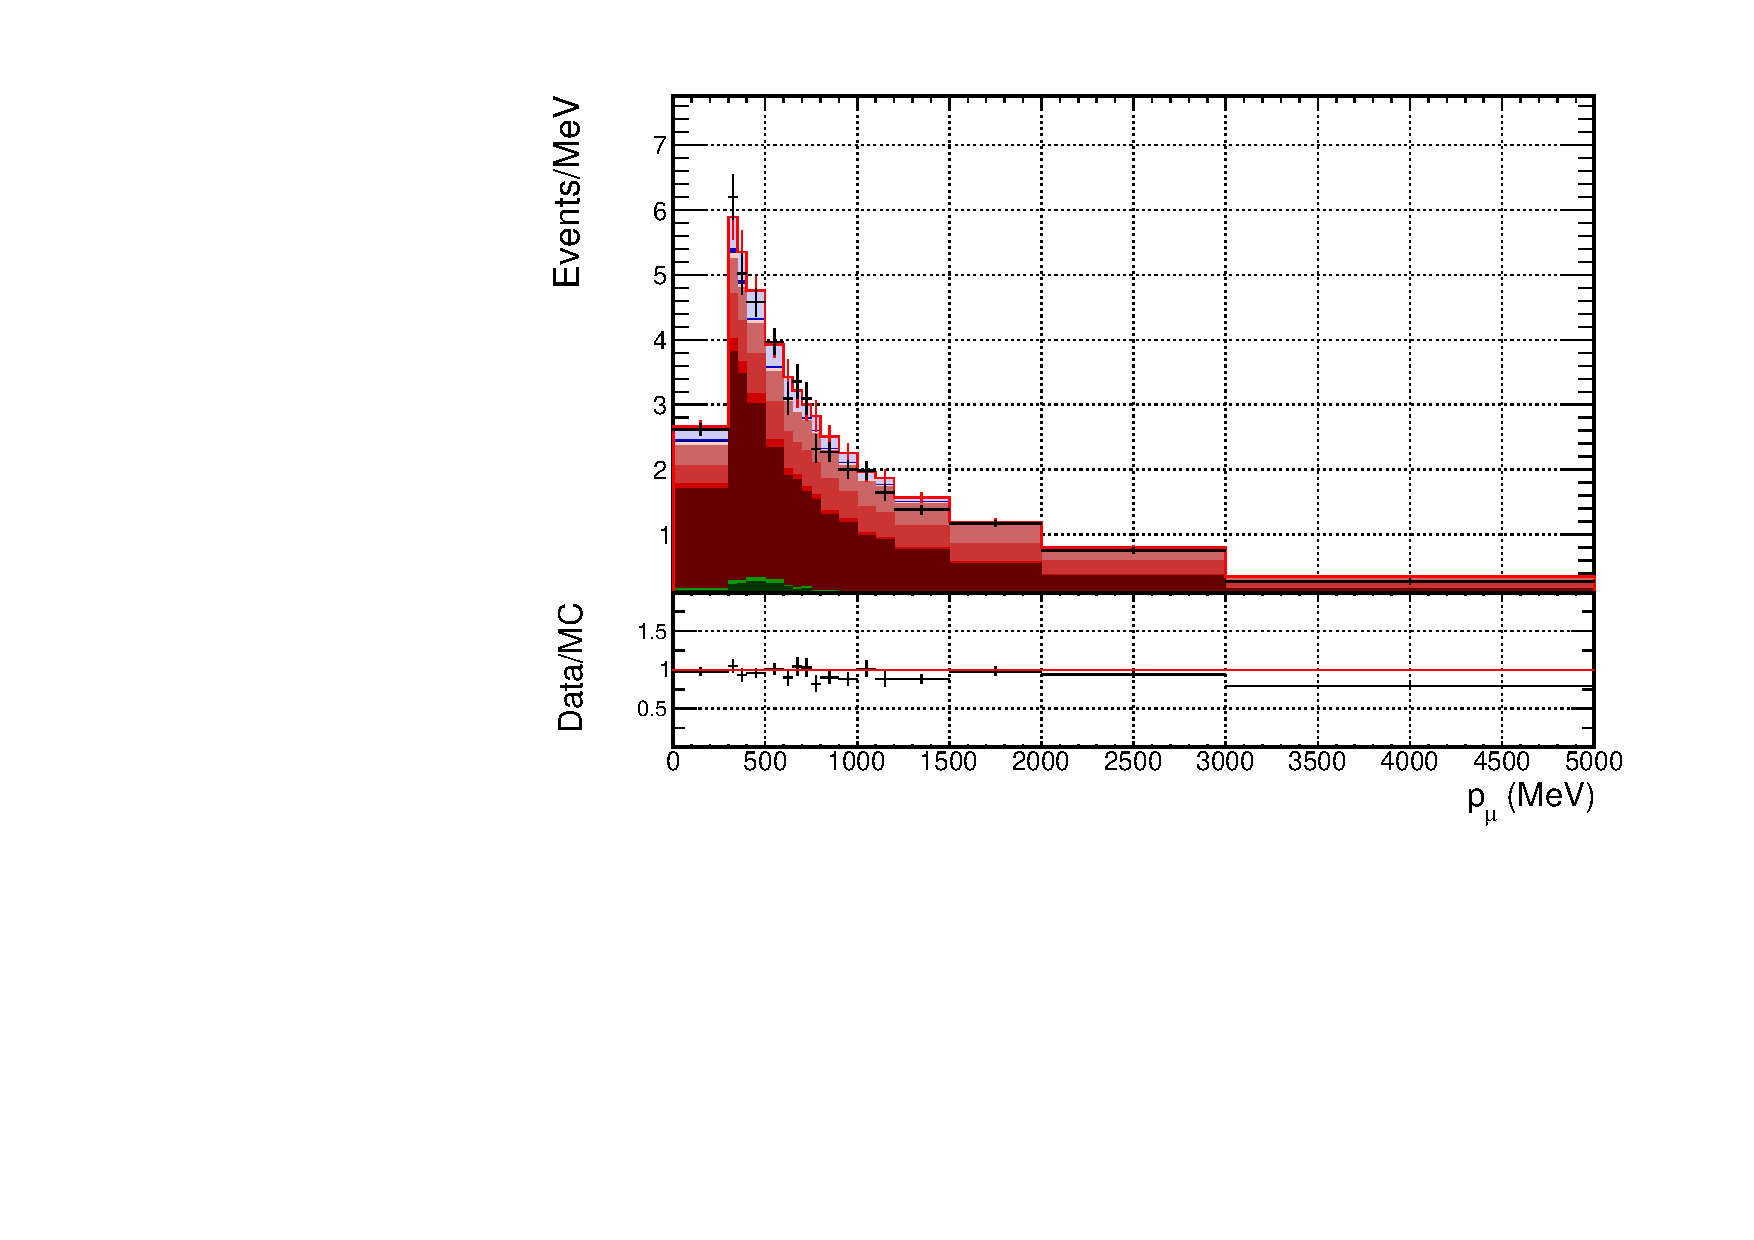
\includegraphics[width=0.95\linewidth]{figs/FGD2_numuCC_1pi_p}
  \caption{FGD2 FHC $\nu_{\mu}$ 1$\pi$}
  \label{fig:pstack_FGD2_numuCC_1pi}
\end{subfigure}
\begin{subfigure}{.32\textwidth}
  \centering
  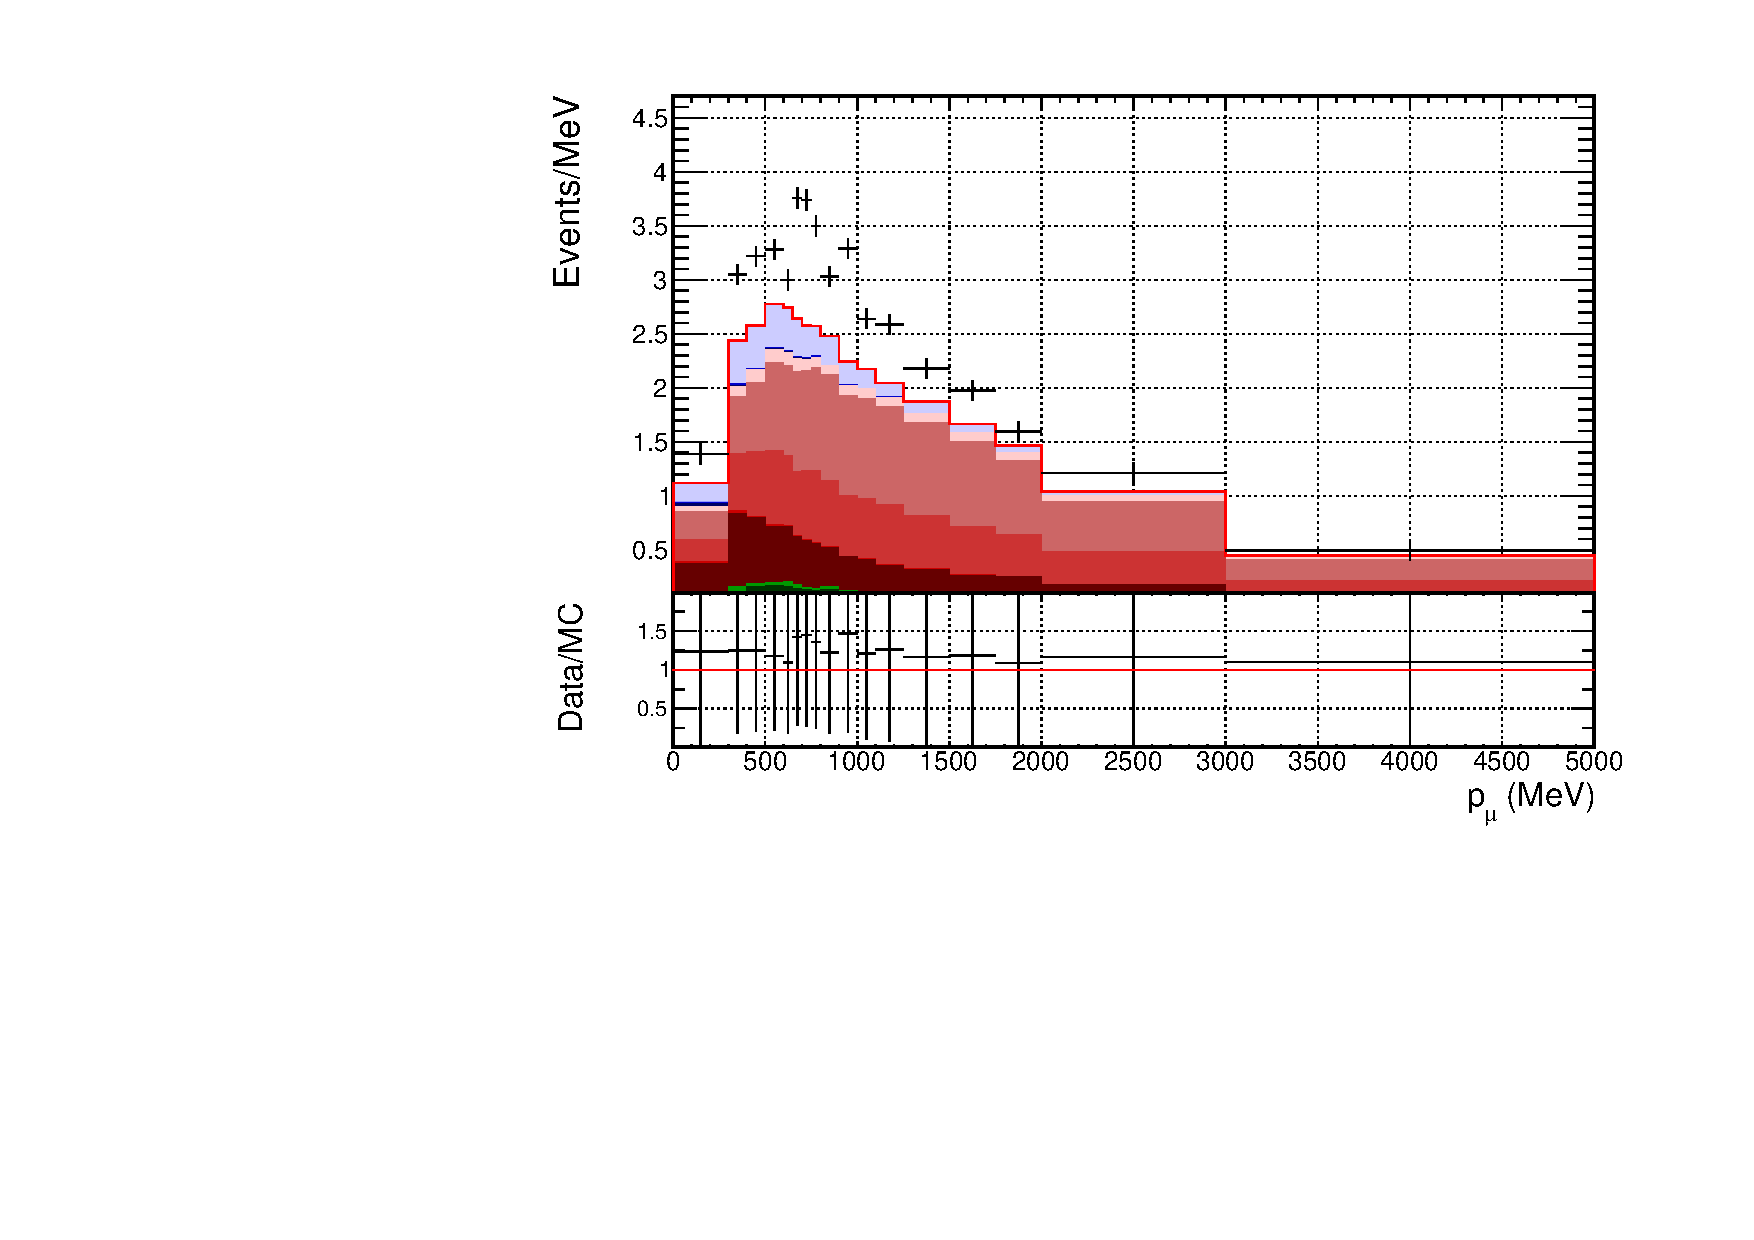
\includegraphics[width=0.95\linewidth]{figs/FGD2_numuCC_other_p}
  \caption{FGD2 FHC $\nu_{\mu}$ Other}
  \label{fig:pstack_FGD2_numuCC_other}
\end{subfigure}
\centering
\begin{subfigure}{.32\textwidth}
  \centering
  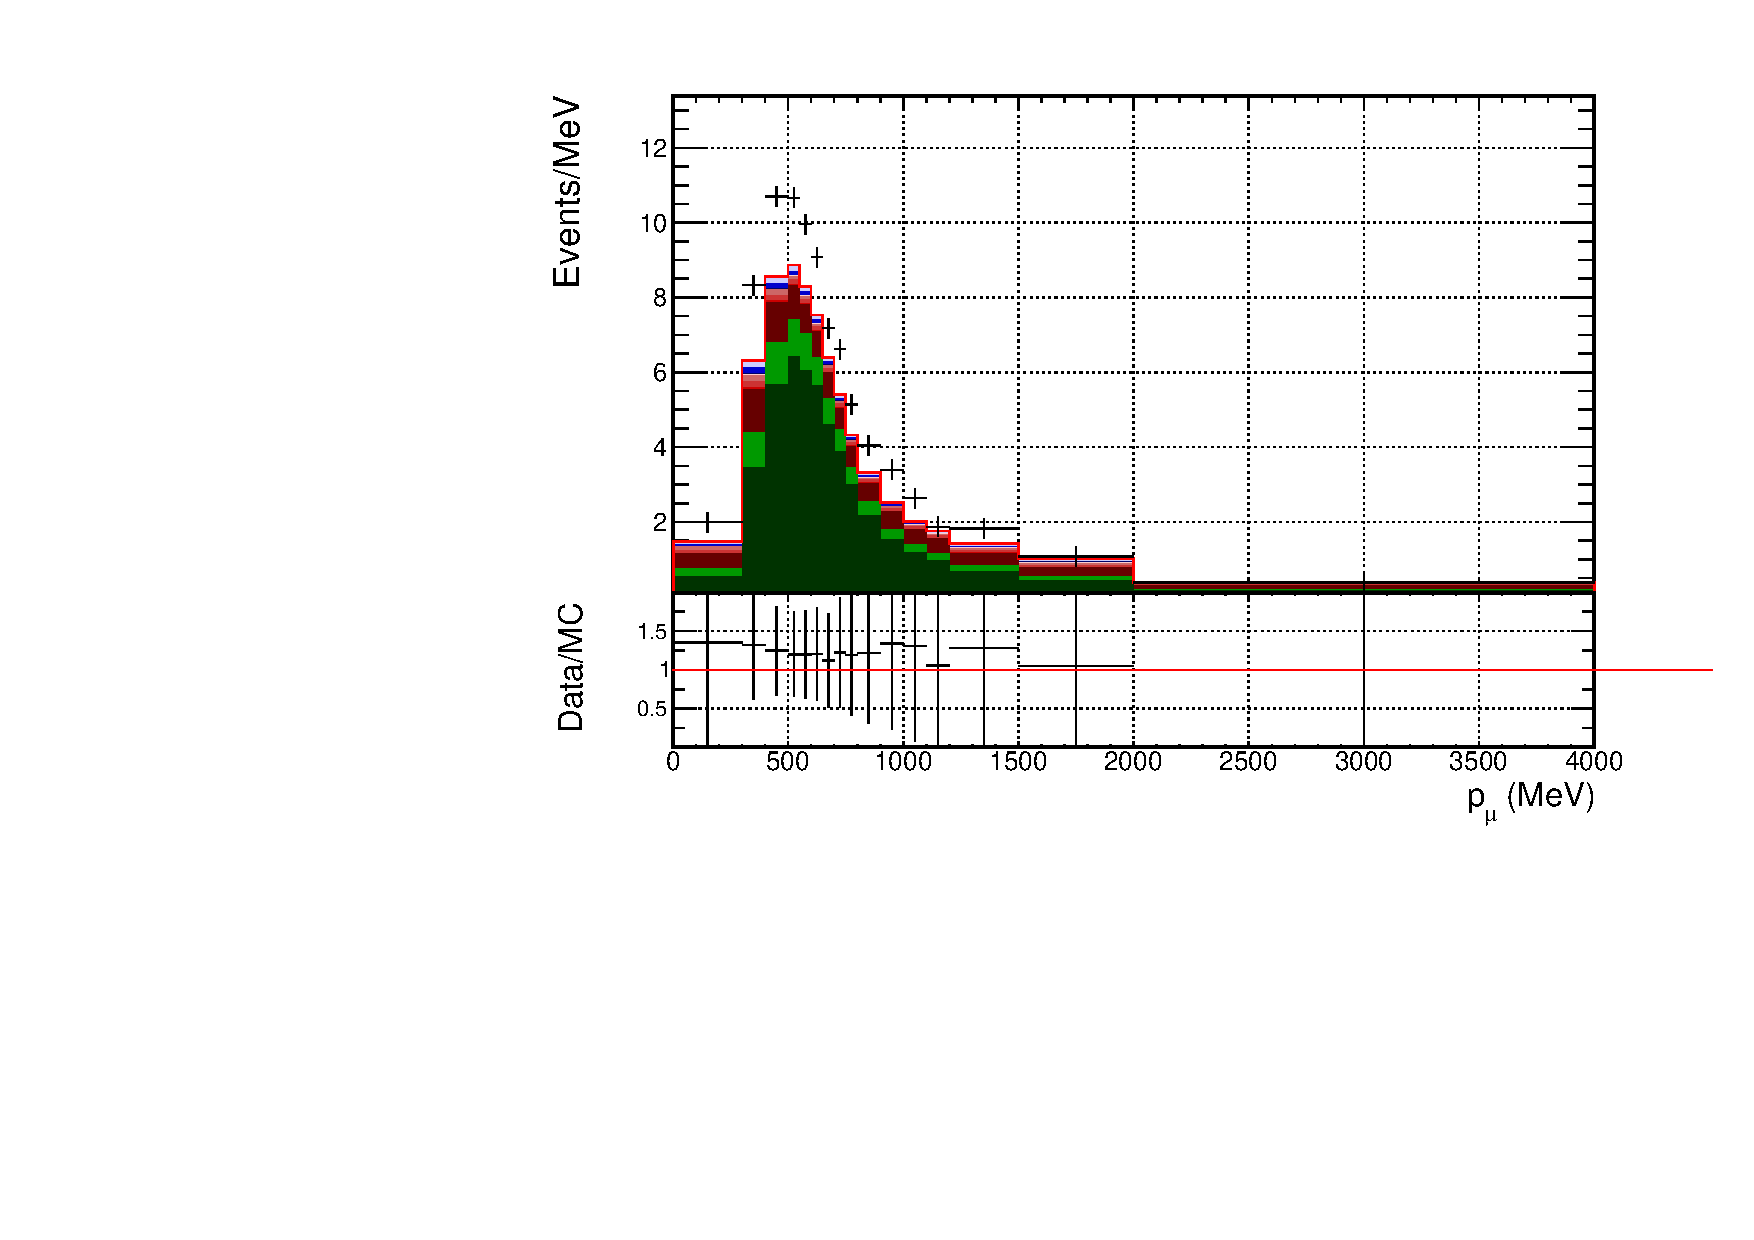
\includegraphics[width=0.95\linewidth]{figs/FGD1_anti-numuCC_0pi_p}
  \caption{FGD1 RHC $\bar{\nu_{\mu}}$ 0$\pi$}
  \label{fig:pstack_FGD1_anti-numuCC_0pi}
\end{subfigure}
\begin{subfigure}{.32\textwidth}
  \centering
  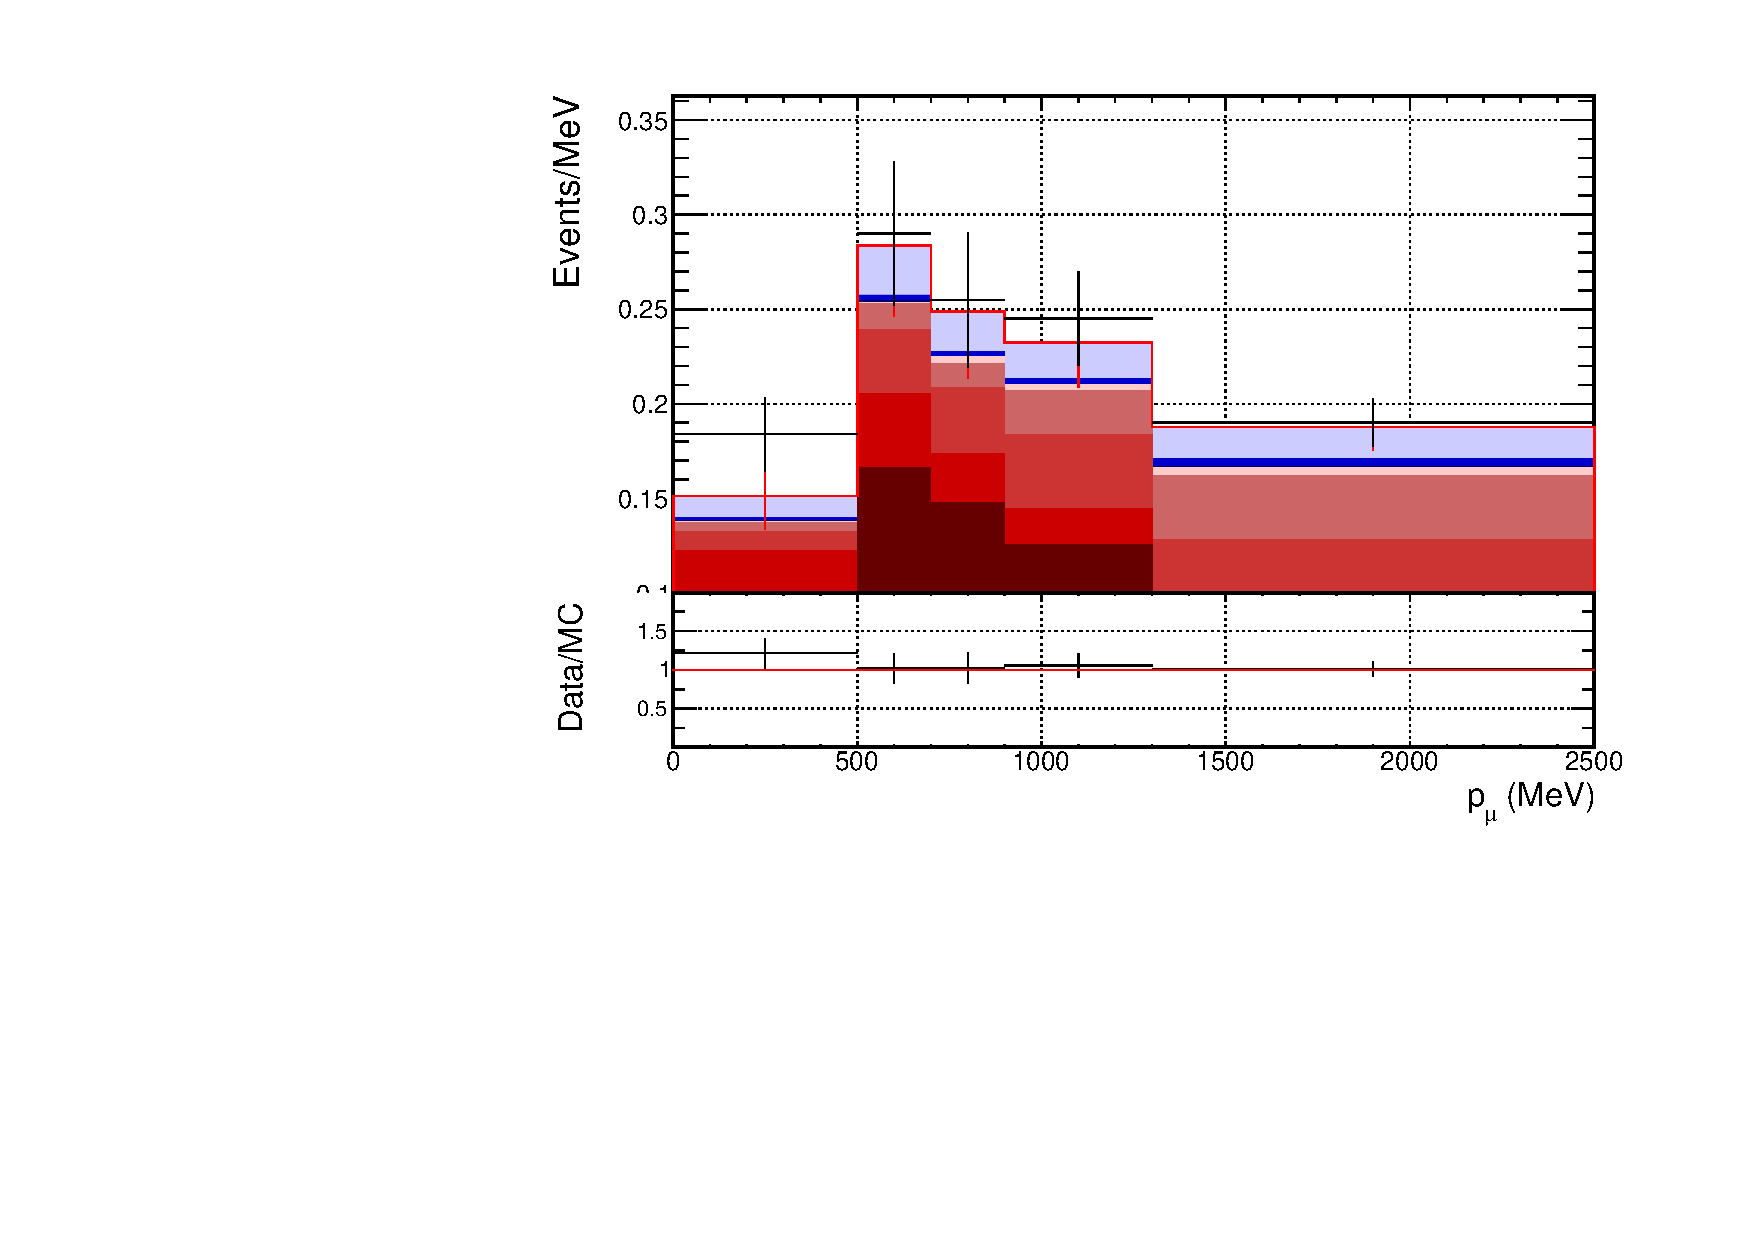
\includegraphics[width=0.95\linewidth]{figs/FGD1_anti-numuCC_1pi_p}
  \caption{FGD1 RHC $\bar{\nu_{\mu}}$ 1$\pi$}
  \label{fig:pstack_pstack_FGD1_anti-numuCC_1pi}
\end{subfigure}
\begin{subfigure}{.32\textwidth}
  \centering
  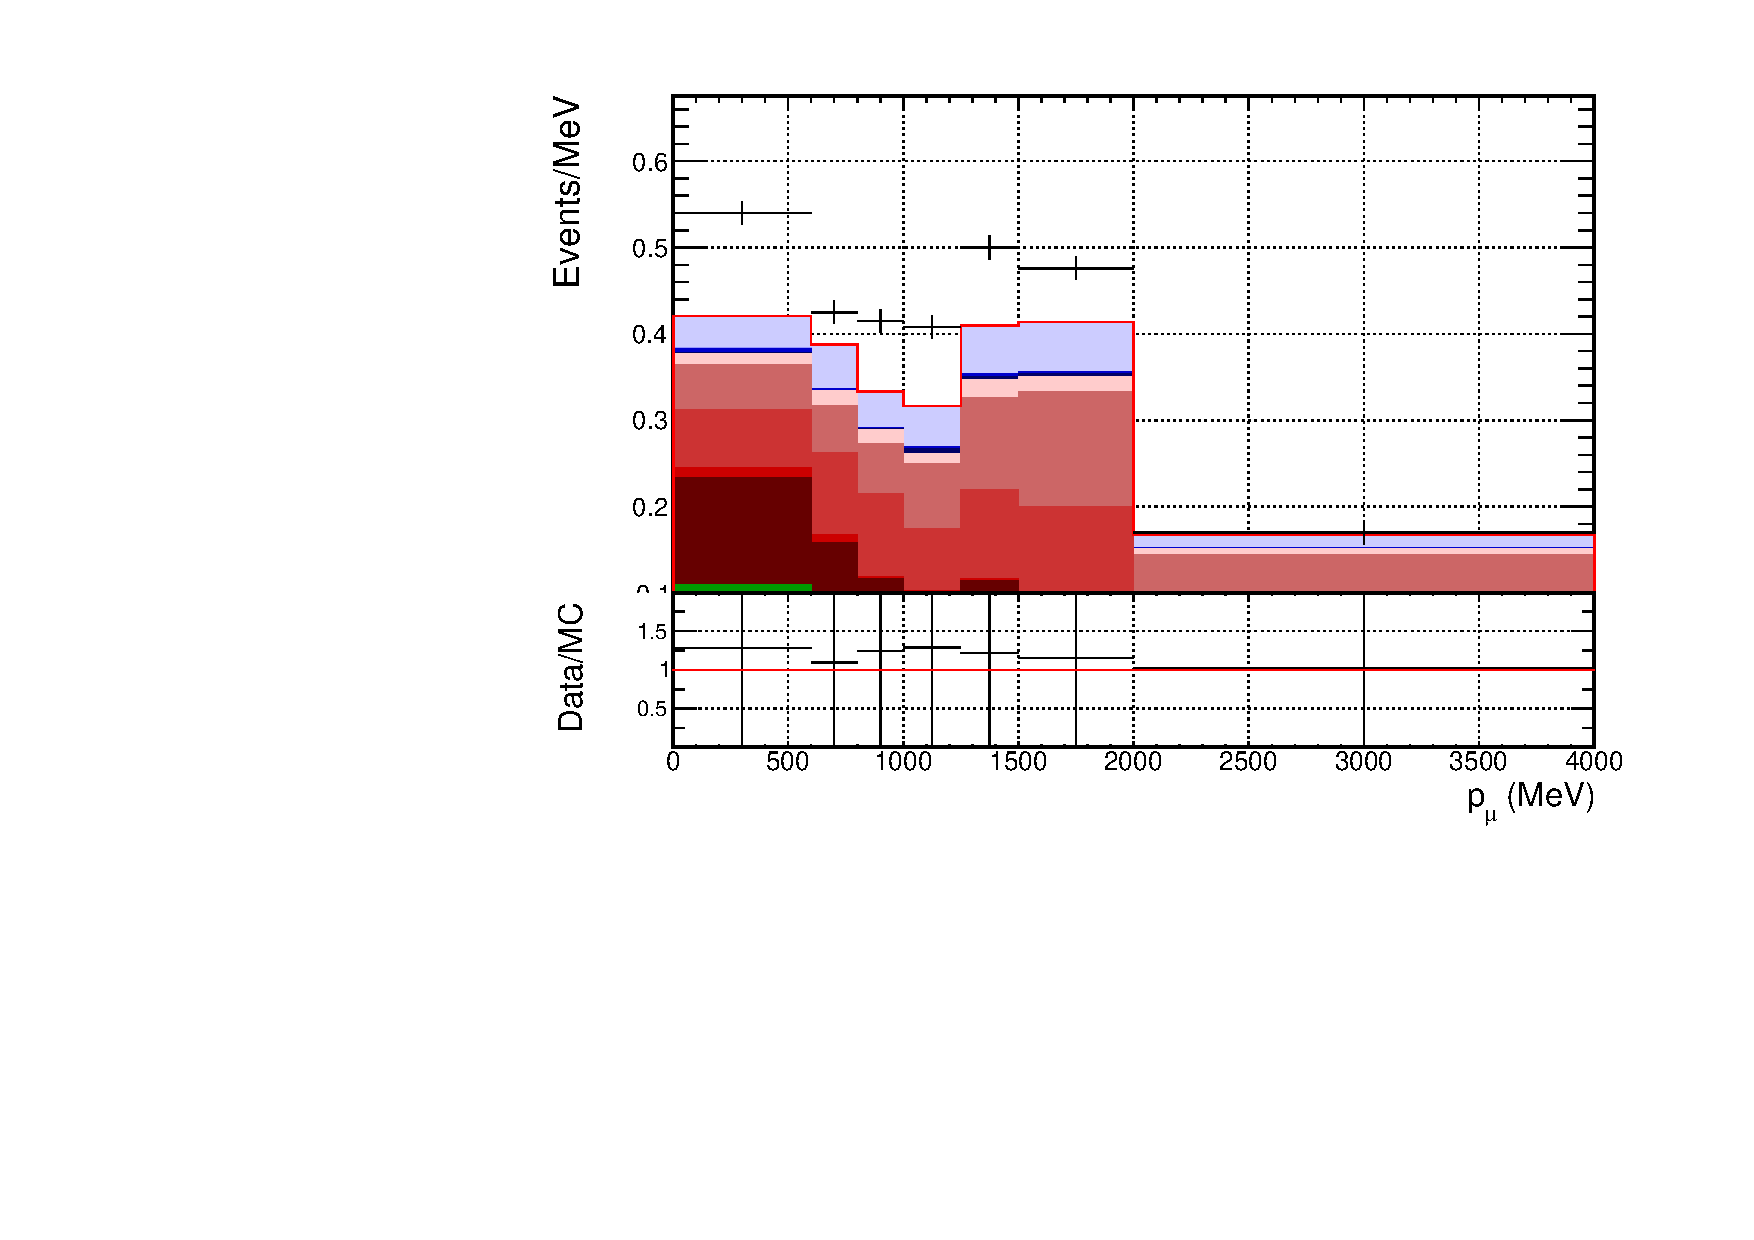
\includegraphics[width=0.95\linewidth]{figs/FGD1_anti-numuCC_other_p}
  \caption{FGD1 RHC $\bar{\nu_{\mu}}$ Other}
  \label{fig:pstack_FGD1_anti-numuCC_other}
\end{subfigure}
\centering
\begin{subfigure}{.32\textwidth}
  \centering
  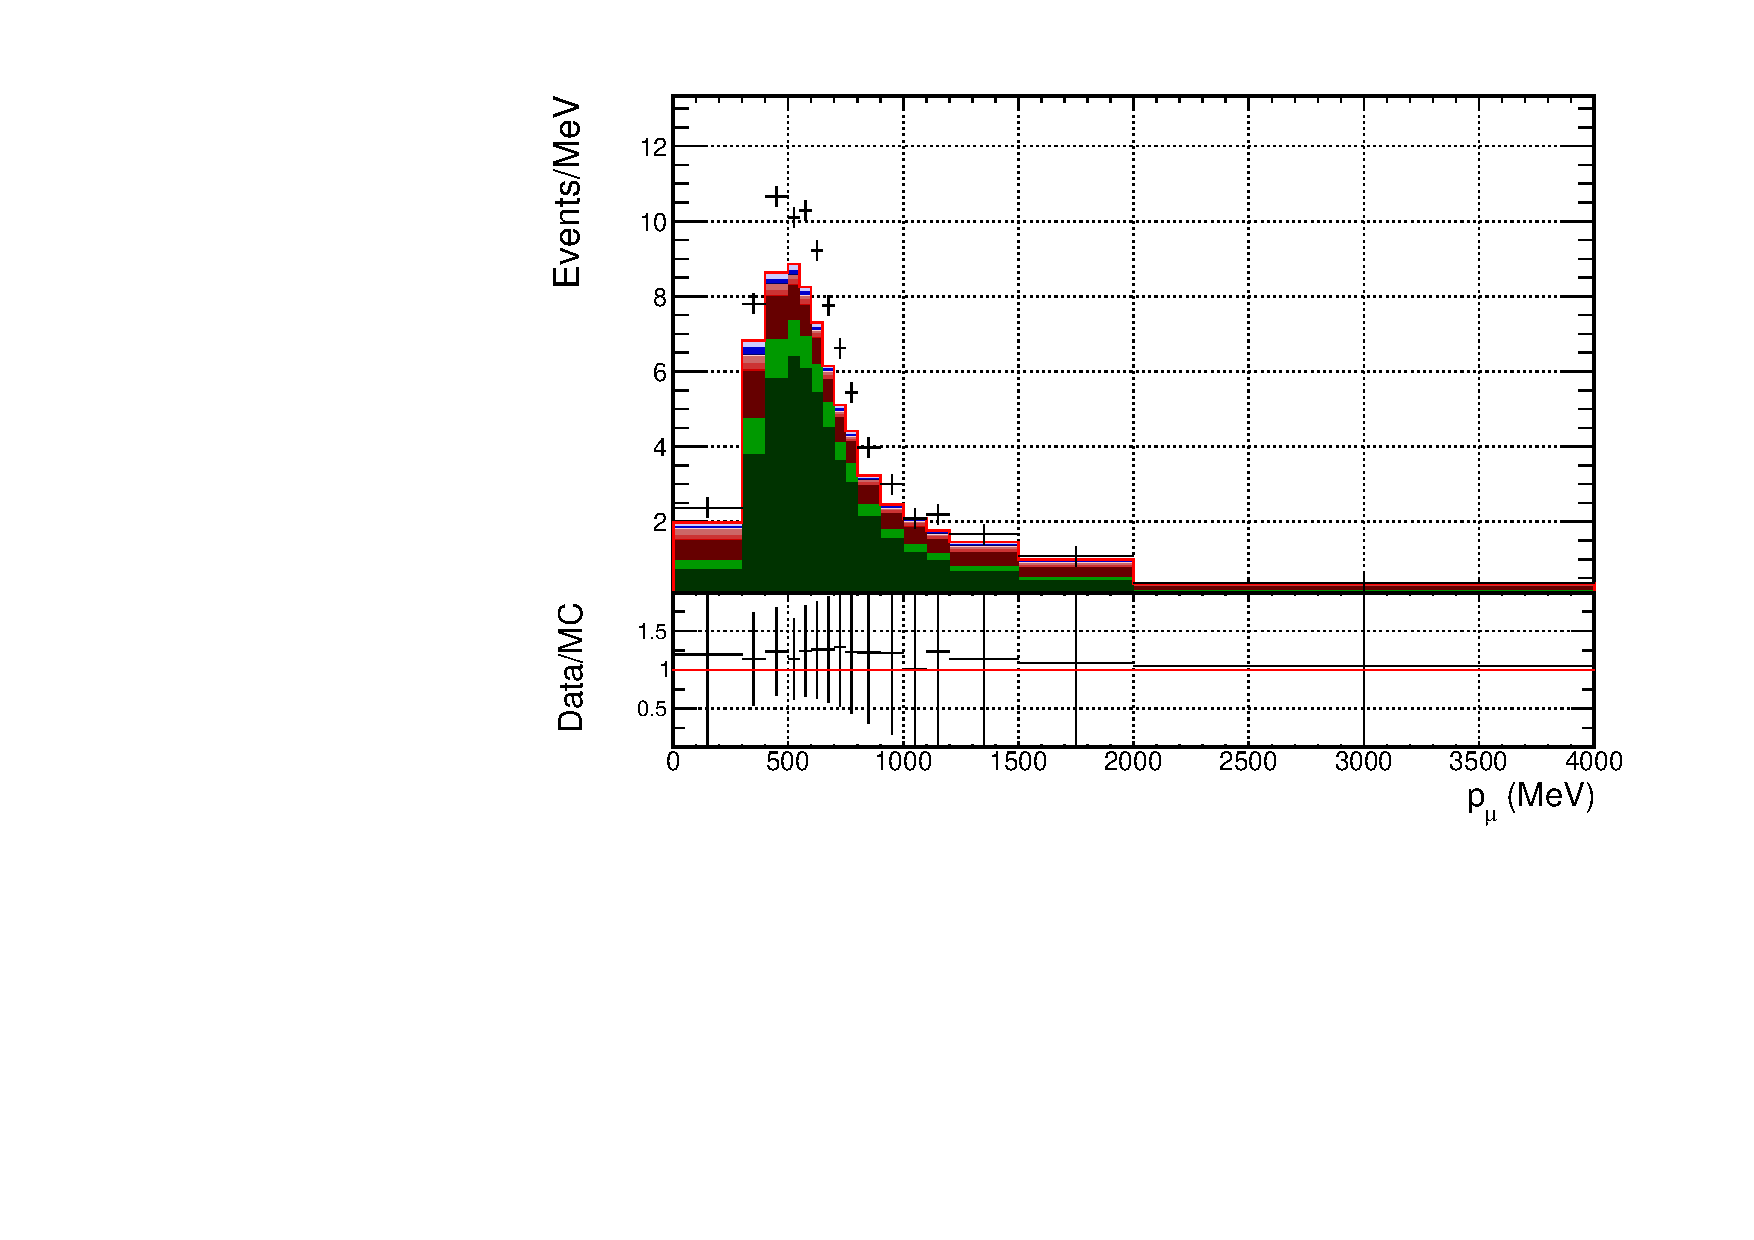
\includegraphics[width=0.95\linewidth]{figs/FGD2_anti-numuCC_0pi_p}
  \caption{FGD2 RHC $\bar{\nu_{\mu}}$ 0$\pi$}
  \label{fig:pstack_FGD2_anti-numuCC_0pi}
\end{subfigure}
\begin{subfigure}{.32\textwidth}
  \centering
  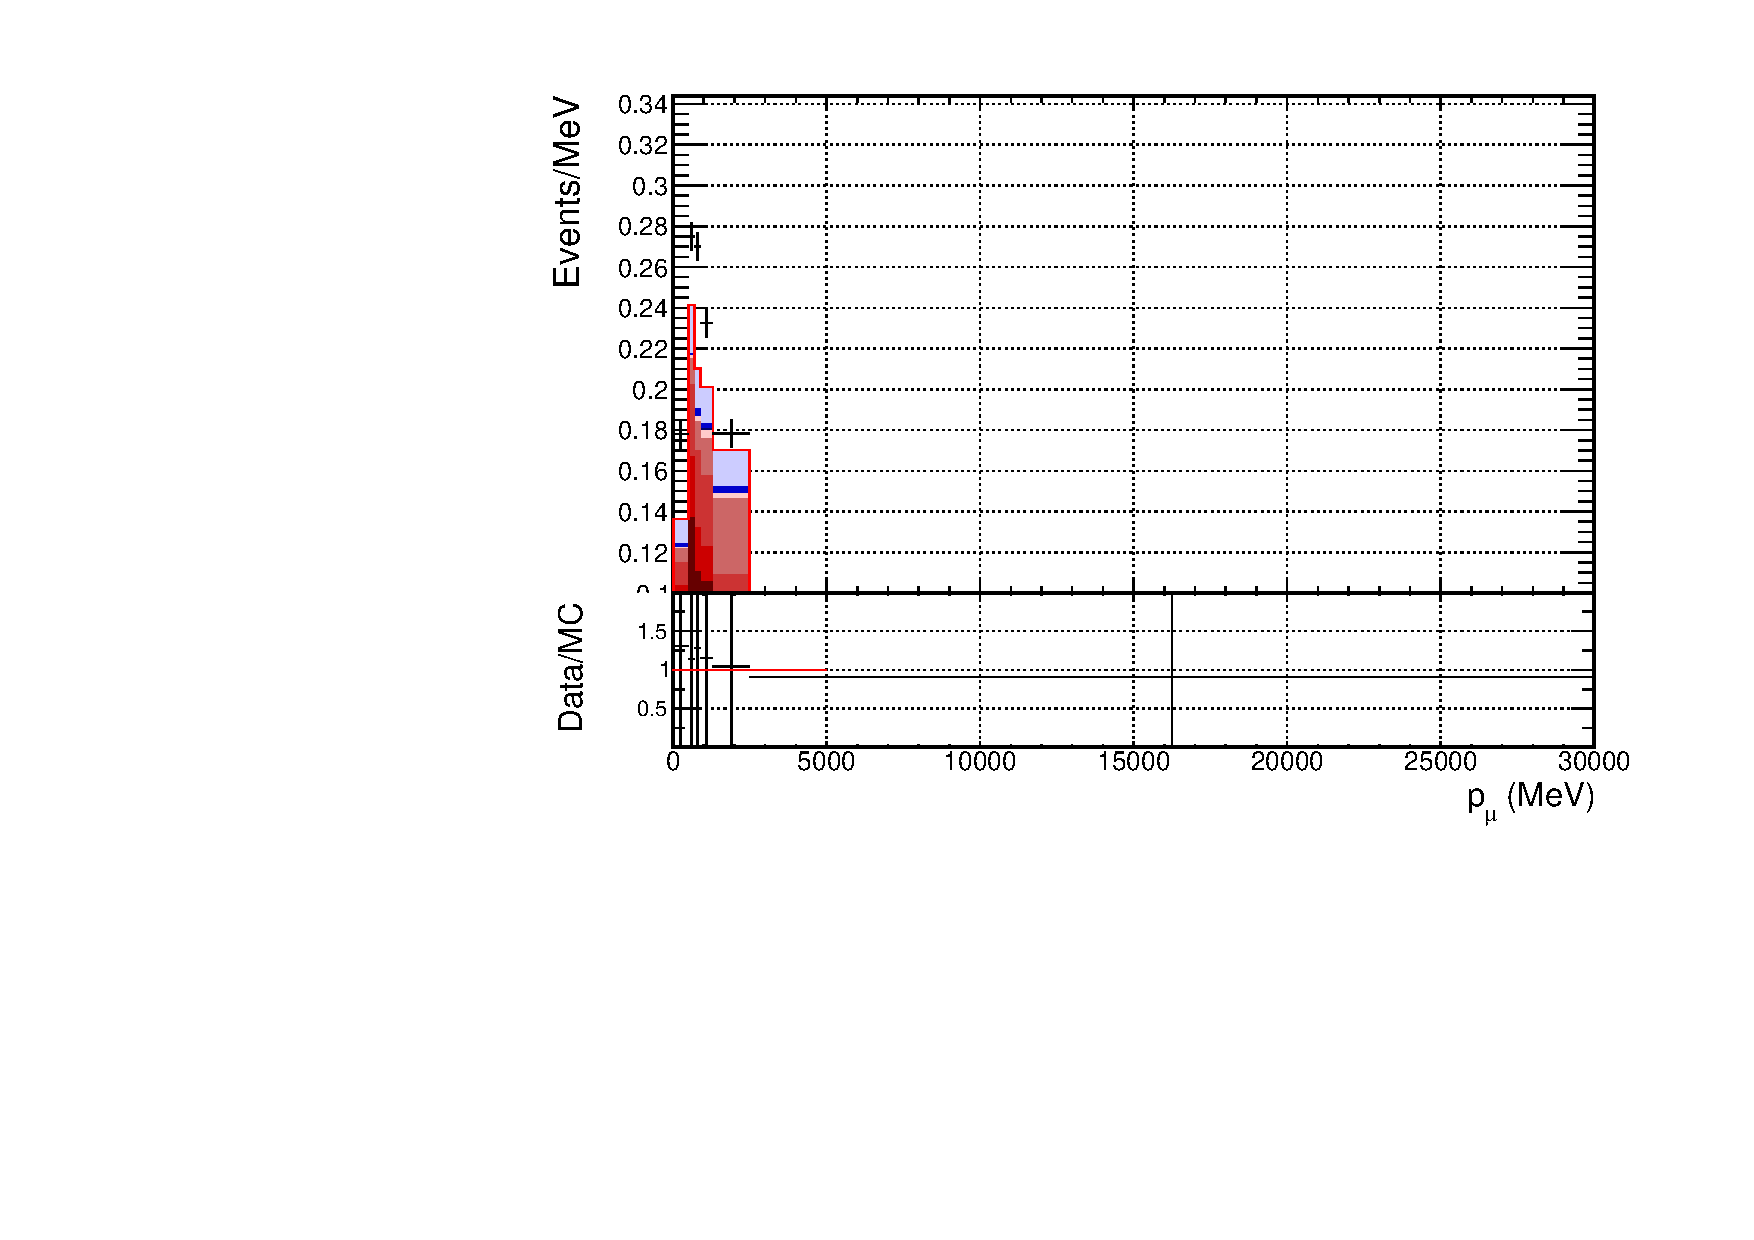
\includegraphics[width=0.95\linewidth]{figs/FGD2_anti-numuCC_1pi_p}
  \caption{FGD2 RHC $\bar{\nu_{\mu}}$ 1$\pi$}
  \label{fig:pstack_pstack_FGD2_anti-numuCC_1pi}
\end{subfigure}
\begin{subfigure}{.32\textwidth}
  \centering
  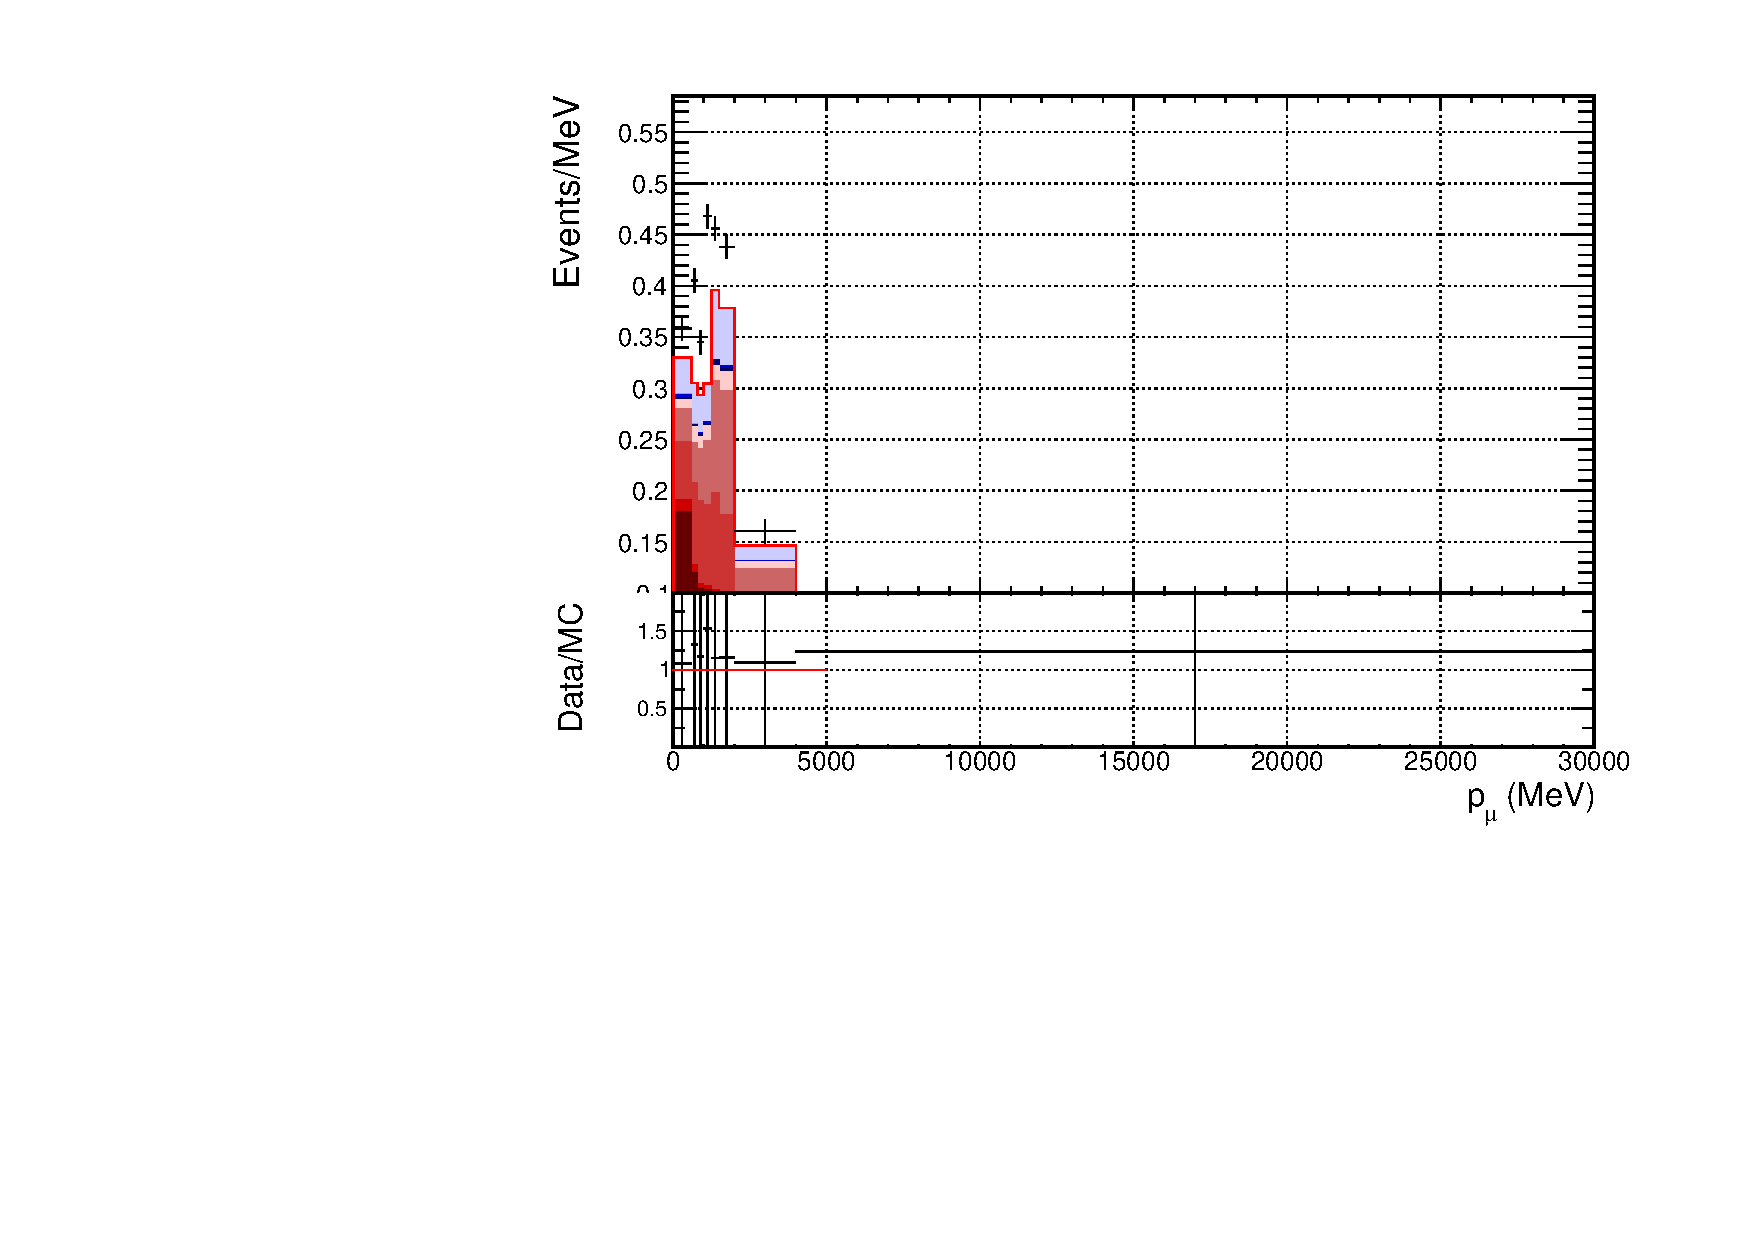
\includegraphics[width=0.95\linewidth]{figs/FGD2_anti-numuCC_other_p}
  \caption{FGD2 RHC $\bar{\nu_{\mu}}$ Other}
  \label{fig:pstack_FGD2_anti-numuCC_other}
\end{subfigure}
\begin{subfigure}{.32\textwidth}
  \centering
  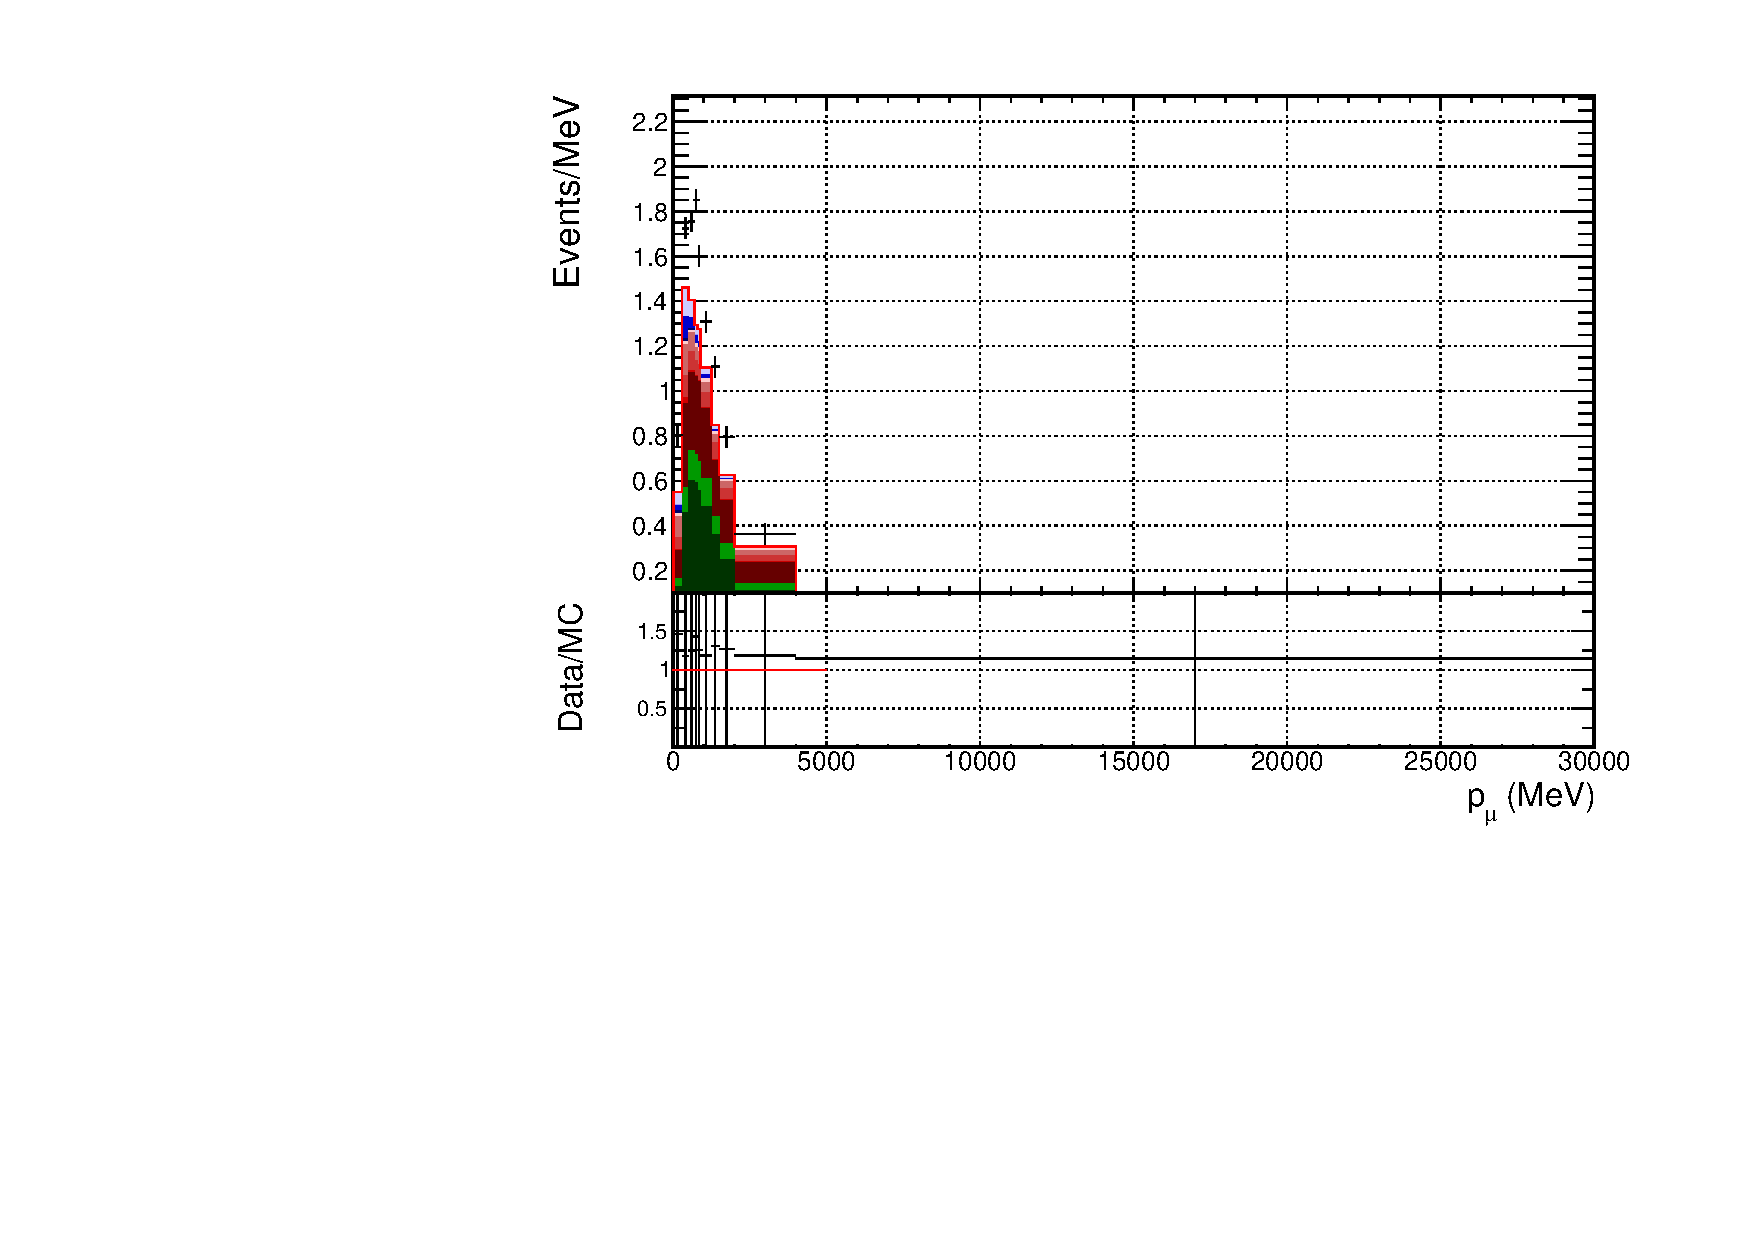
\includegraphics[width=0.95\linewidth]{figs/FGD1_NuMuBkg_CC0pi_in_AntiNu_Mode_p}
  \caption{FGD1 RHC $\nu_{\mu}$ 0$\pi$}
  \label{fig:pstack_FGD1_NuMuBkg_CC0pi_in_AntiNu_Mode}
\end{subfigure}
\begin{subfigure}{.32\textwidth}
  \centering
  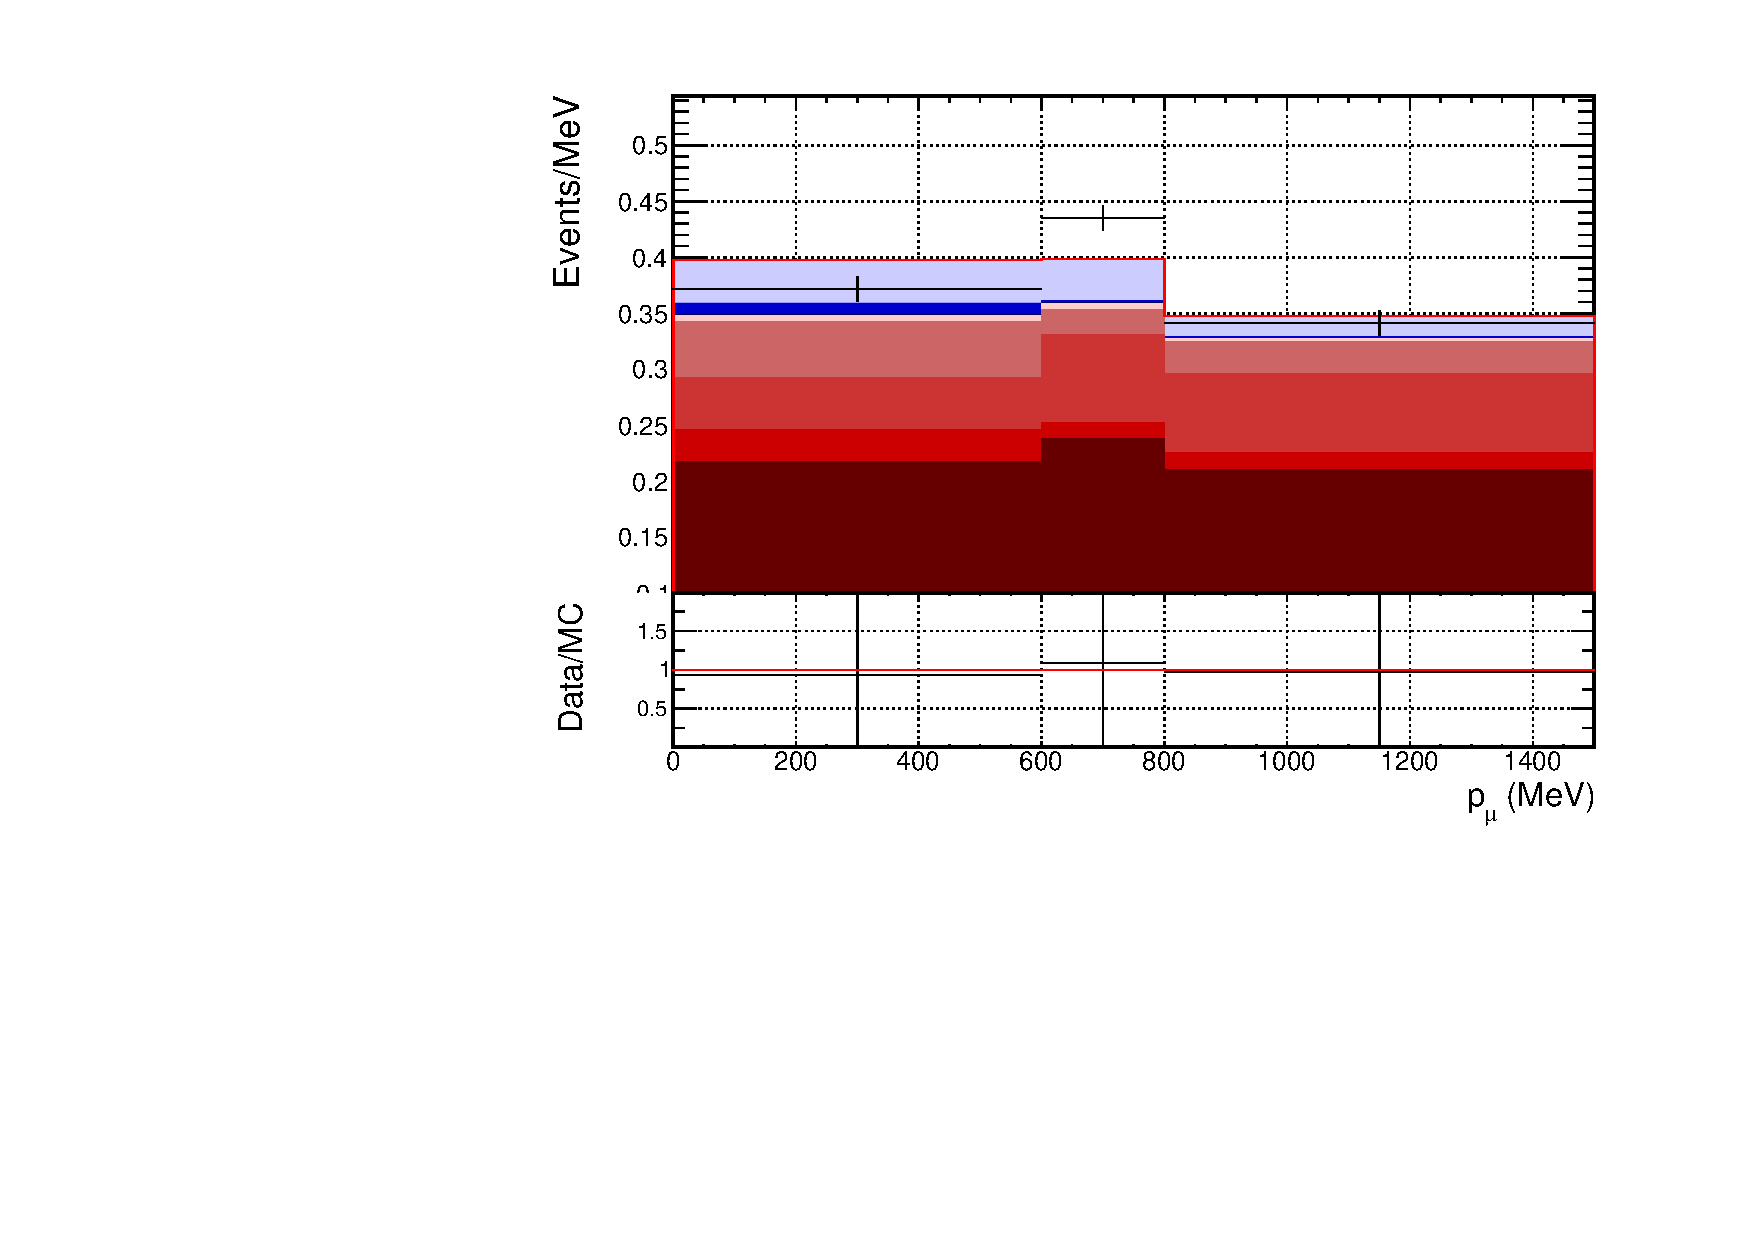
\includegraphics[width=0.95\linewidth]{figs/FGD1_NuMuBkg_CC1pi_in_AntiNu_Mode_p}
  \caption{FGD1 RHC $\nu_{\mu}$ 1$\pi$}
  \label{fig:pstack_FGD1_NuMuBkg_CC1pi_in_AntiNu_Mode}
\end{subfigure}
\begin{subfigure}{.32\textwidth}
  \centering
  \includegraphics[width=0.95\linewidth]{figs/FGD1_NuMuBkg_CCOther_in_AntiNu_Mode_p}
  \caption{FGD1 RHC $\nu_{\mu}$ Other}
  \label{fig:pstack_FGD1_NuMuBkg_CCOther_in_AntiNu_Mode}
\end{subfigure}
\begin{subfigure}{.32\textwidth}
  \centering
  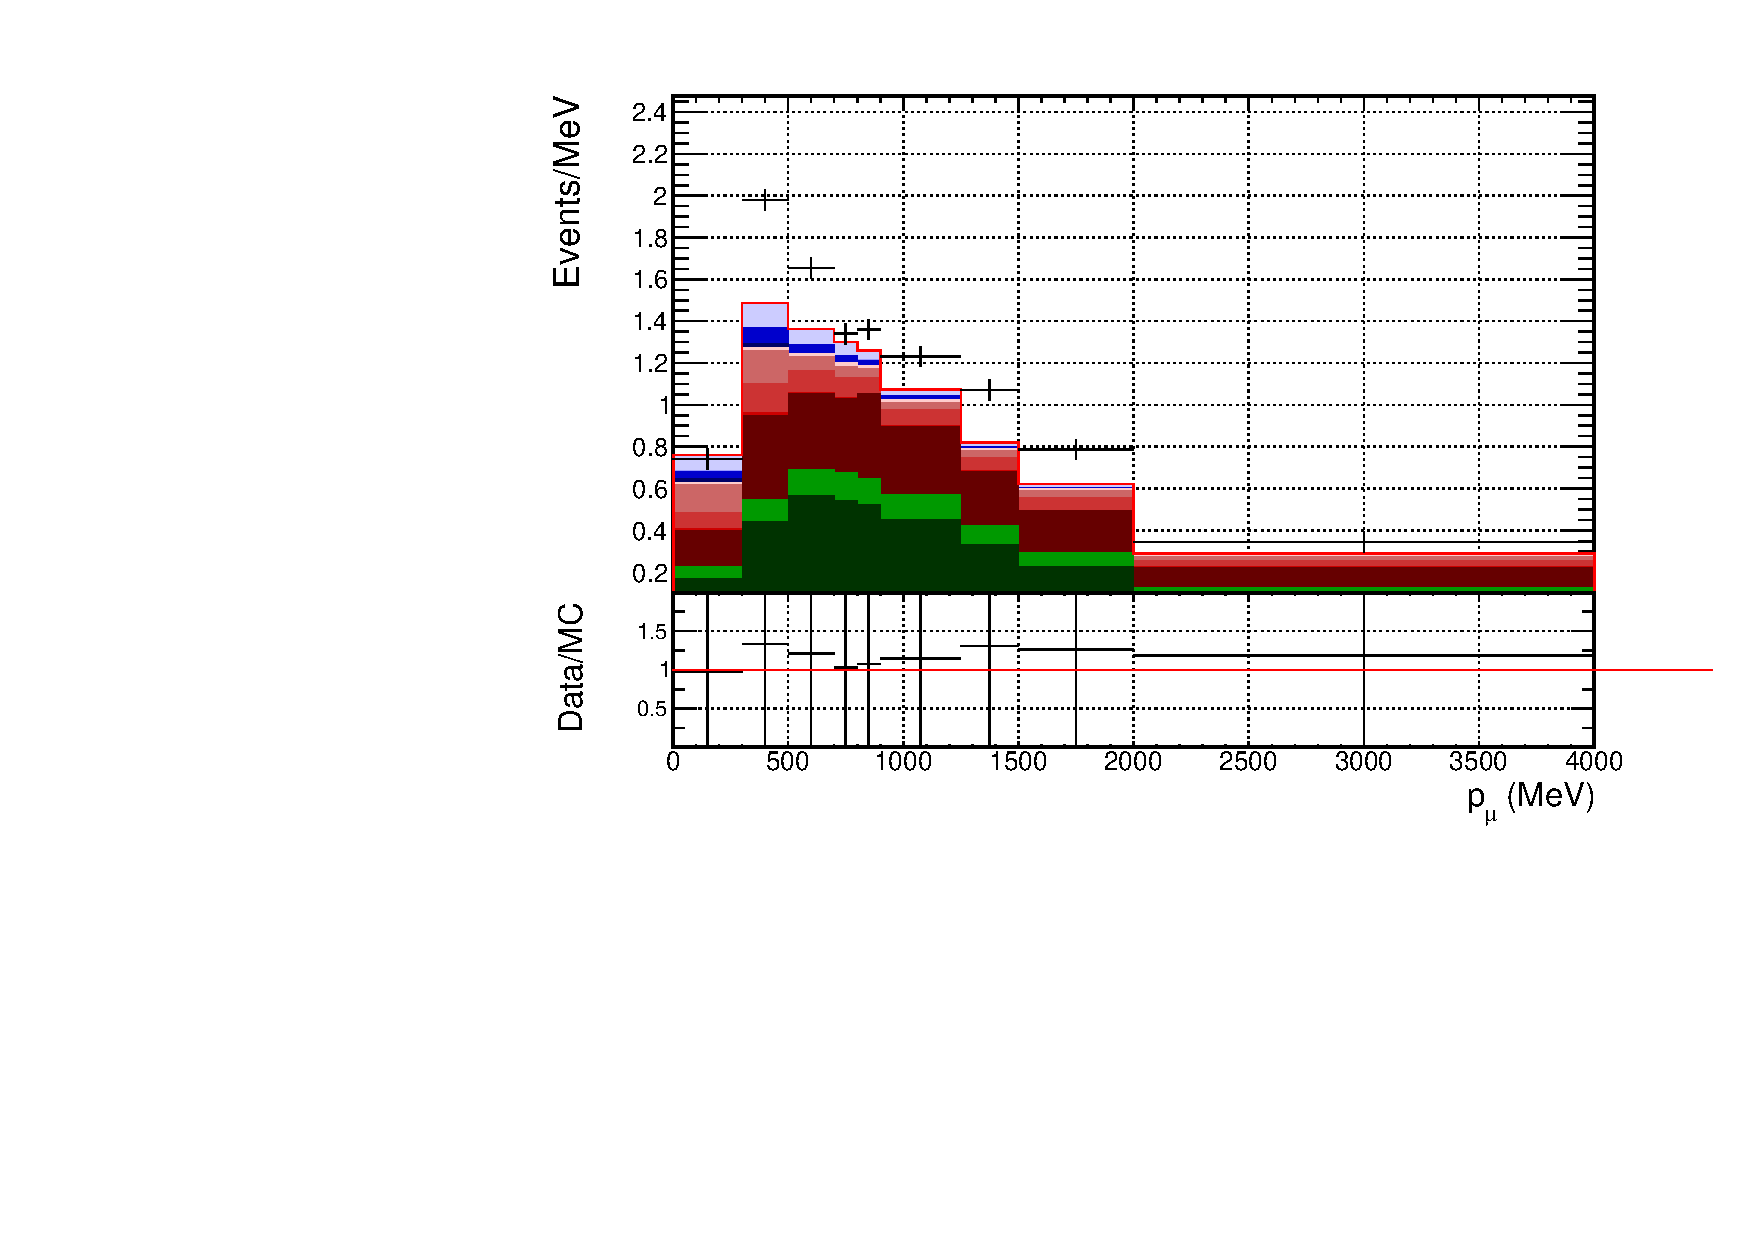
\includegraphics[width=0.95\linewidth]{figs/FGD2_NuMuBkg_CC0pi_in_AntiNu_Mode_p}
  \caption{FGD2 RHC $\nu_{\mu}$ 0$\pi$}
  \label{fig:pstack_FGD2_NuMuBkg_CC0pi_in_AntiNu_Mode}
\end{subfigure}
\begin{subfigure}{.32\textwidth}
  \centering
  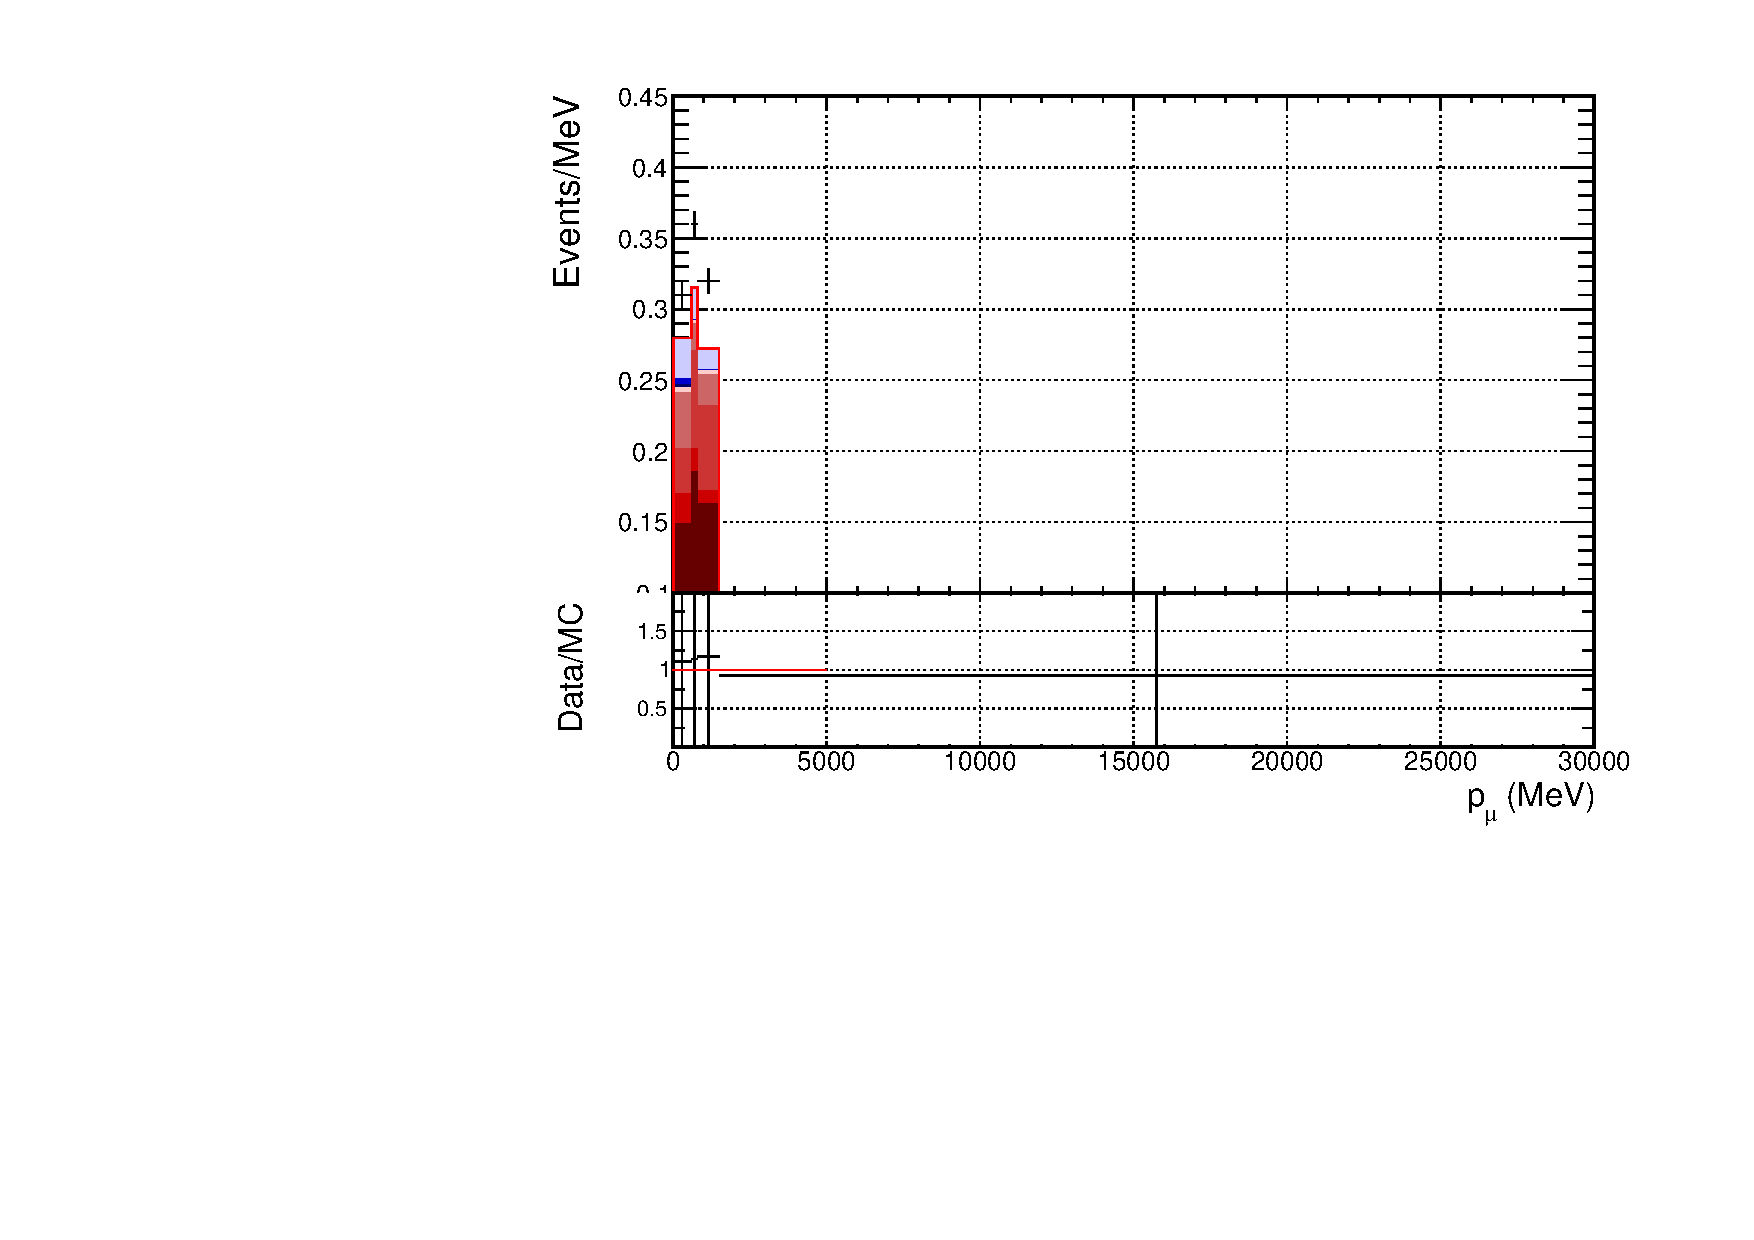
\includegraphics[width=0.95\linewidth]{figs/FGD2_NuMuBkg_CC1pi_in_AntiNu_Mode_p}
  \caption{FGD2 RHC $\nu_{\mu}$ 1$\pi$}
  \label{fig:pstack_FGD2_NuMuBkg_CC1pi_in_AntiNu_Mode}
\end{subfigure}
\begin{subfigure}{.32\textwidth}
  \centering
  \includegraphics[width=0.95\linewidth]{figs/FGD2_NuMuBkg_CCOther_in_AntiNu_Mode_p}
  \caption{FGD2 RHC $\nu_{\mu}$ Other}
  \label{fig:pstack_FGD2_NuMuBkg_CCOther_in_AntiNu_Mode}
\end{subfigure}
\caption{p$_{\mu}$ projections of data and nominal MC broken down by interaction mode.}
\label{fig:pstack}
\end{figure}

The projections onto the cos $\theta_{\mu}$ axis are shown in Figure \ref{fig:tstack}, along with the data and interaction mode breakdown.

The CC 0$\pi$ and CC Other samples again show oscillatory behaviour in the ratio of data to MC. At high angle, the ratio increases and decreases, but always remains $>1$. For the CC 1$\pi$ samples,  the ratio is again more flat, but at high angle oscillates between the MC over and underestimating the data. This is again consistent across the FGDs.

\begin{figure}
\centering
\begin{subfigure}{.35\textwidth}
  \centering
  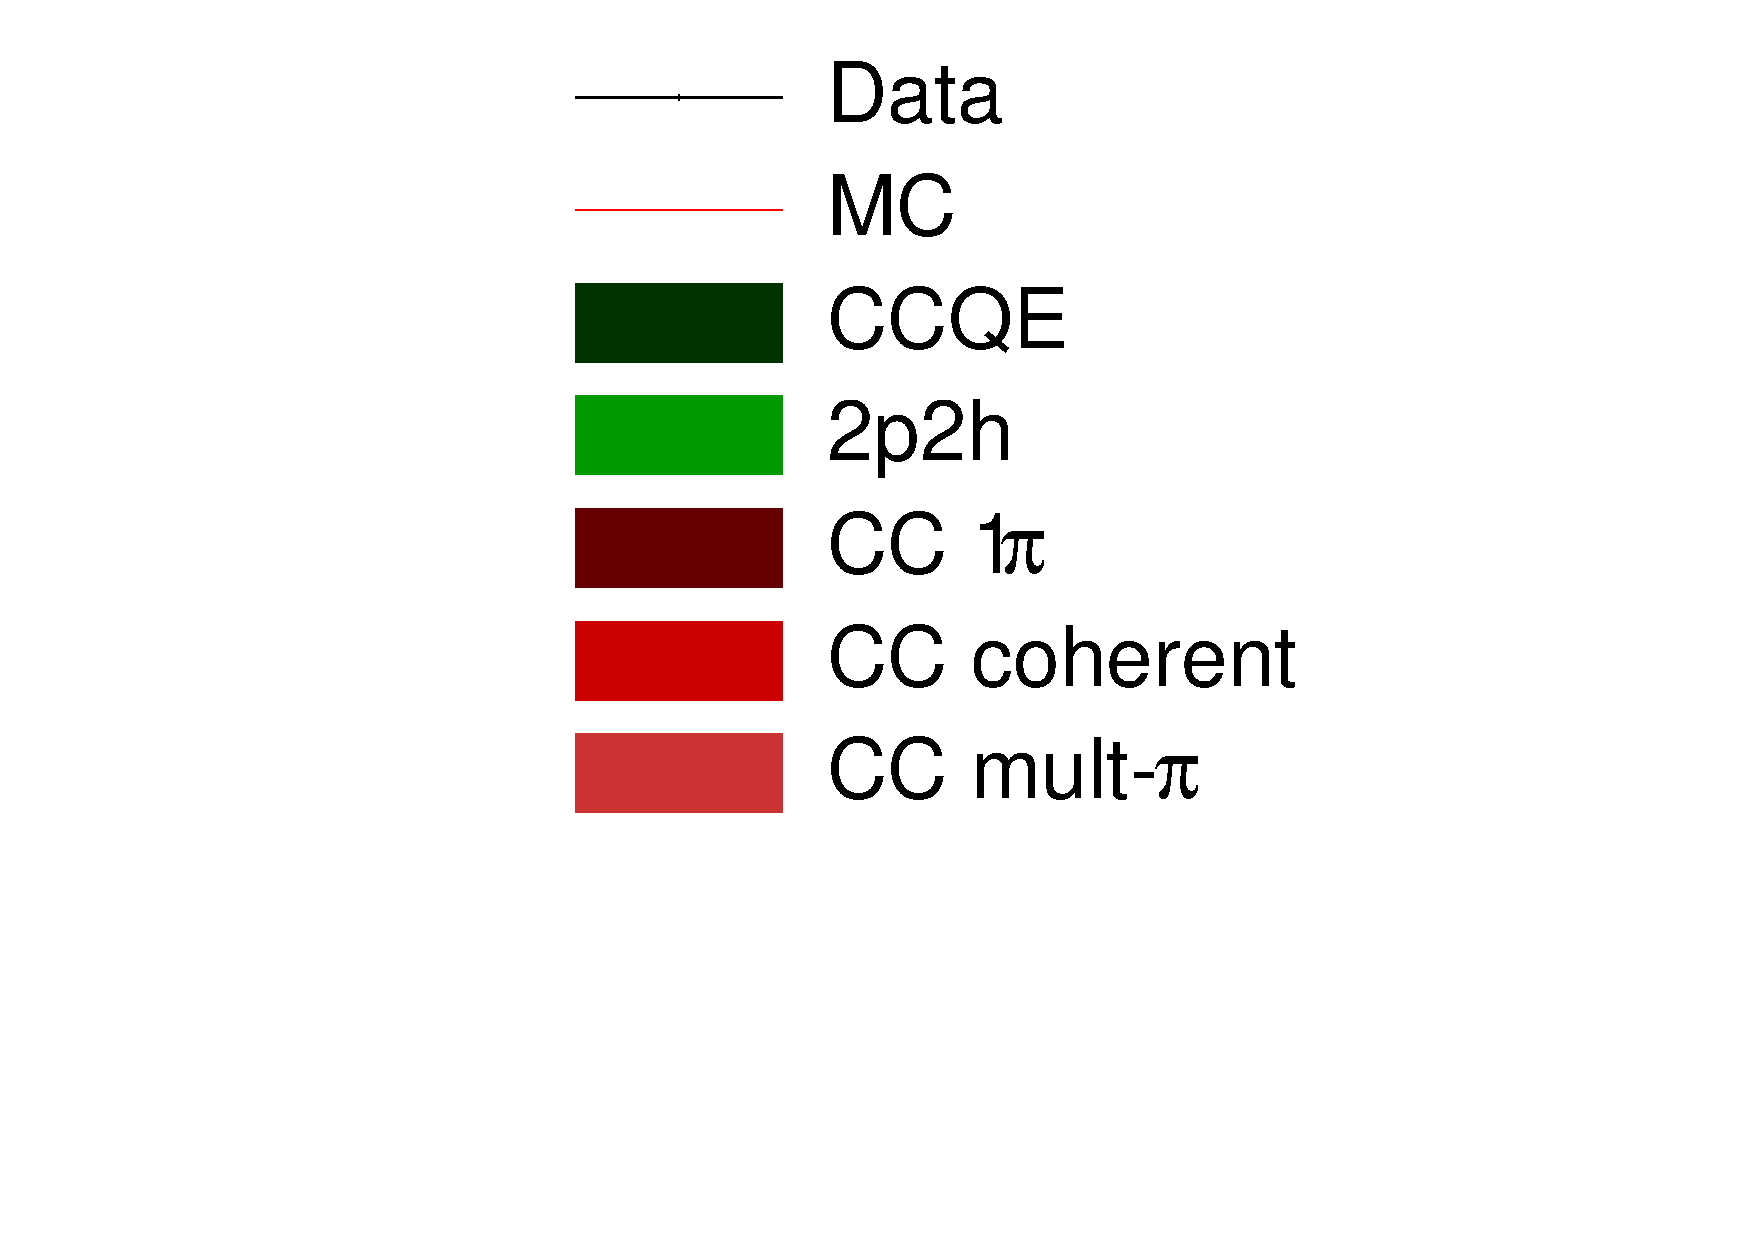
\includegraphics[width=0.7\linewidth]{figs/legend}
\end{subfigure}
\begin{subfigure}{.35\textwidth}
  \centering
  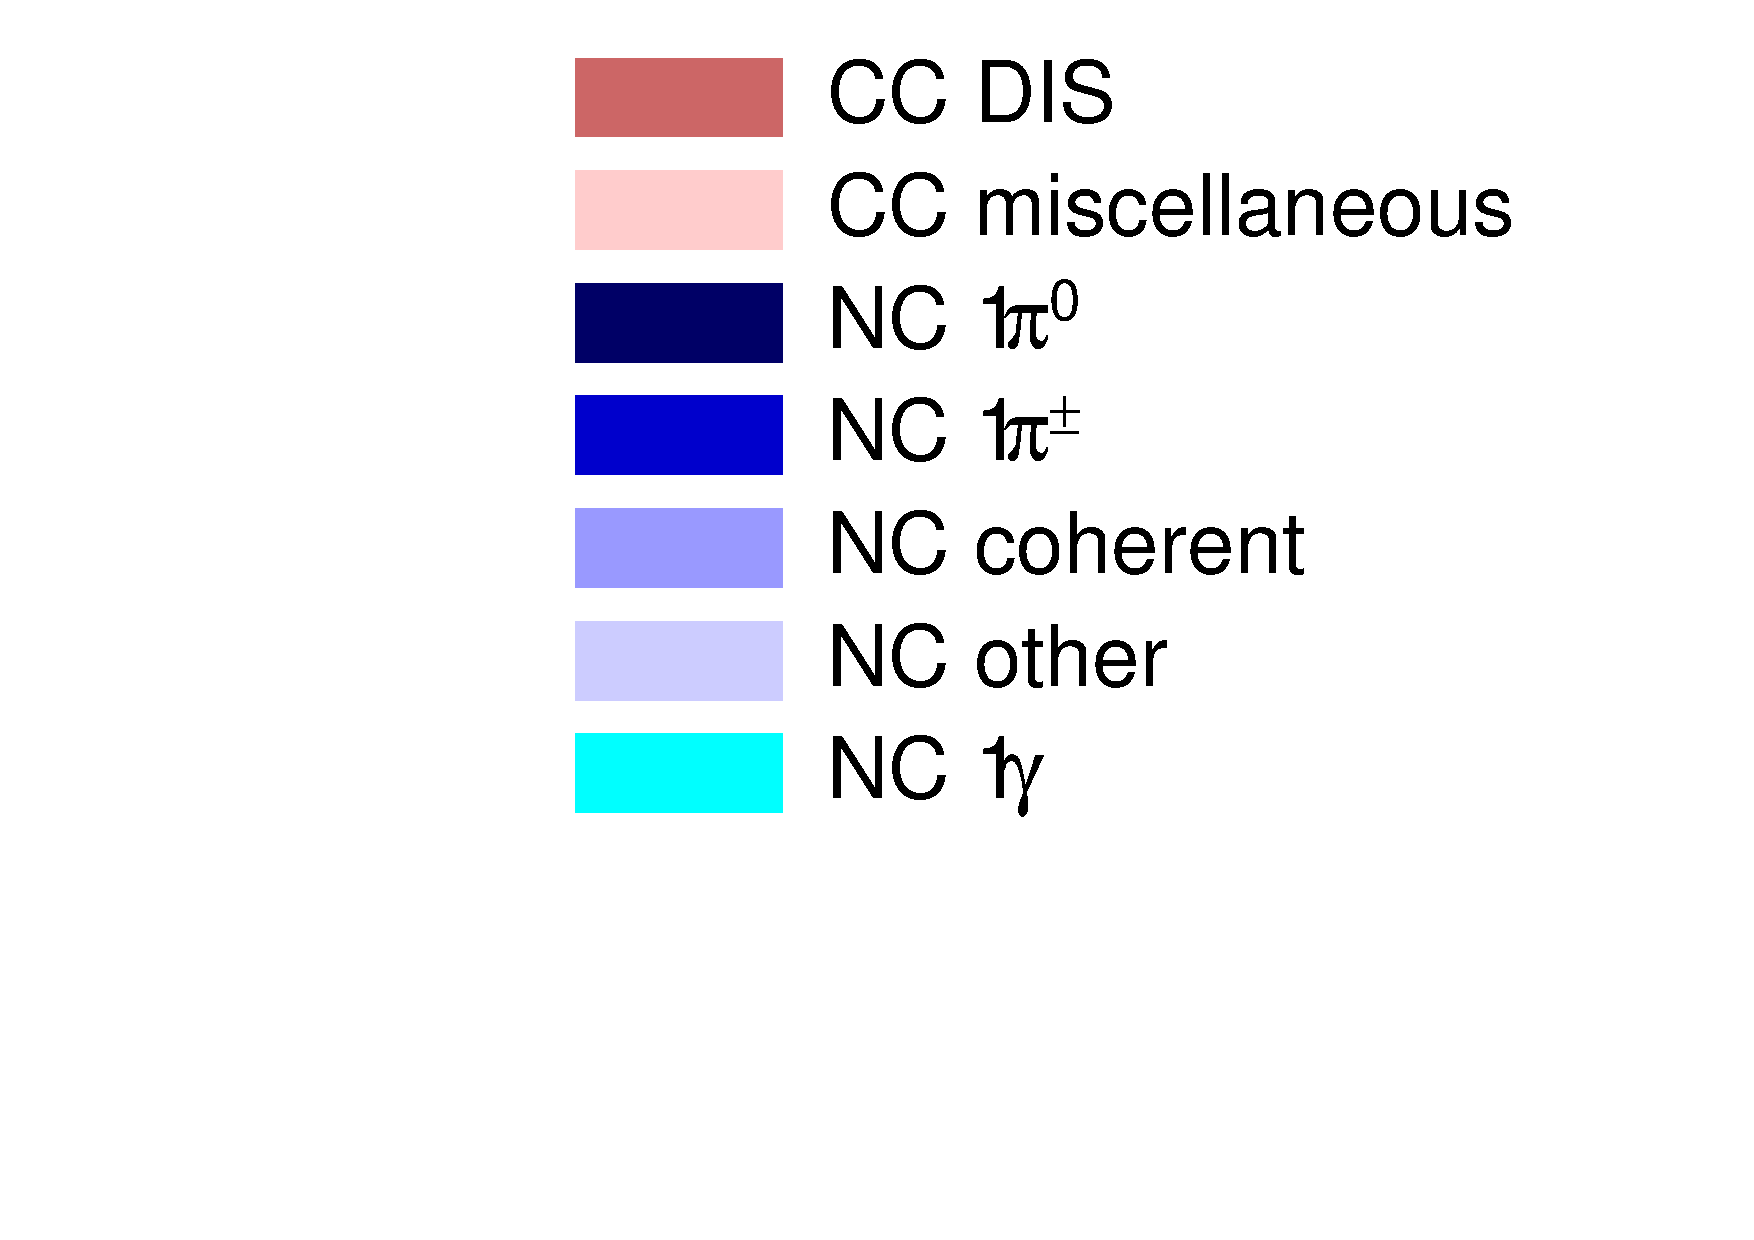
\includegraphics[width=0.7\linewidth]{figs/legend2}
\end{subfigure}
\begin{subfigure}{.32\textwidth}
  \centering
  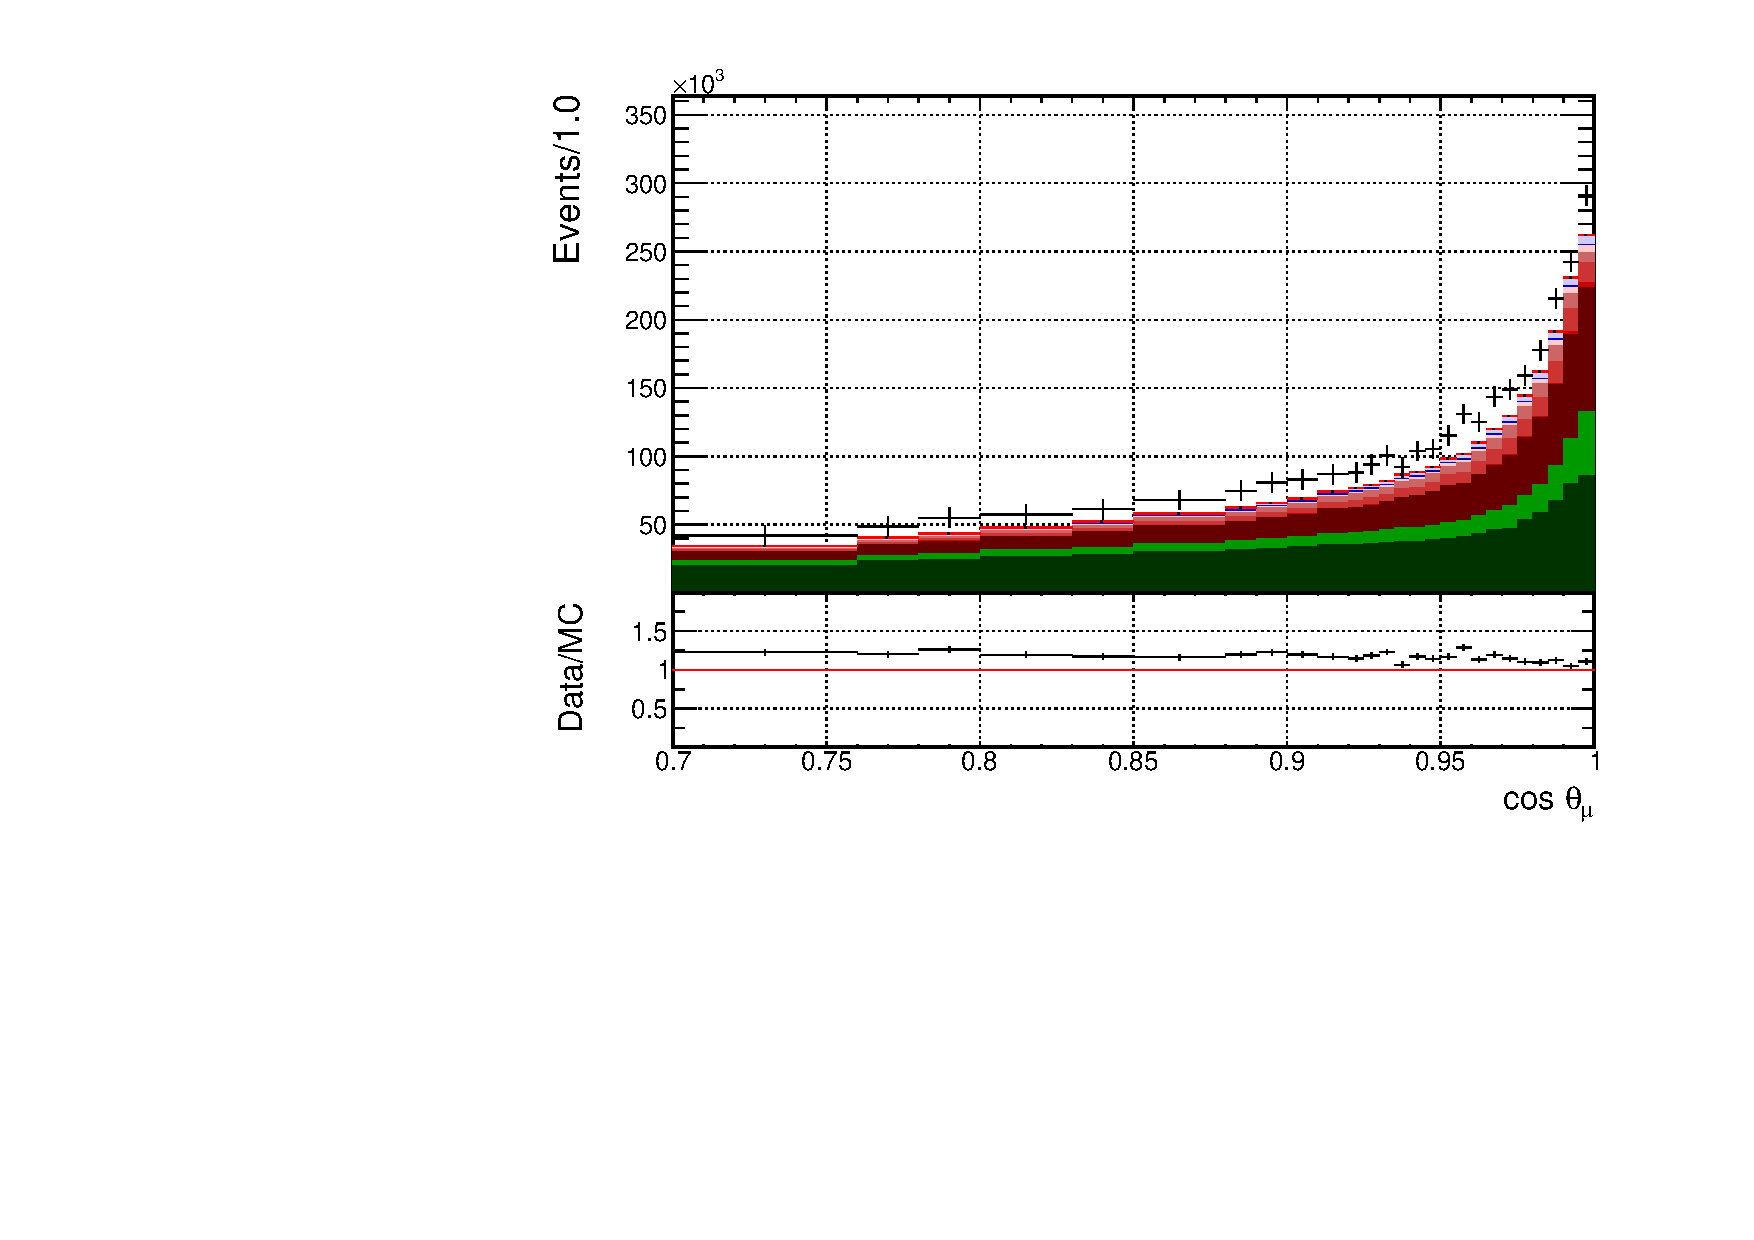
\includegraphics[width=0.95\linewidth]{figs/FGD1_numuCC_0pi_t}
  \caption{FGD1 FHC $\nu_{\mu}$ 0$\pi$}
  \label{fig:tstack_FGD1_numuCC_0pi}
\end{subfigure}
\begin{subfigure}{.32\textwidth}
  \centering
  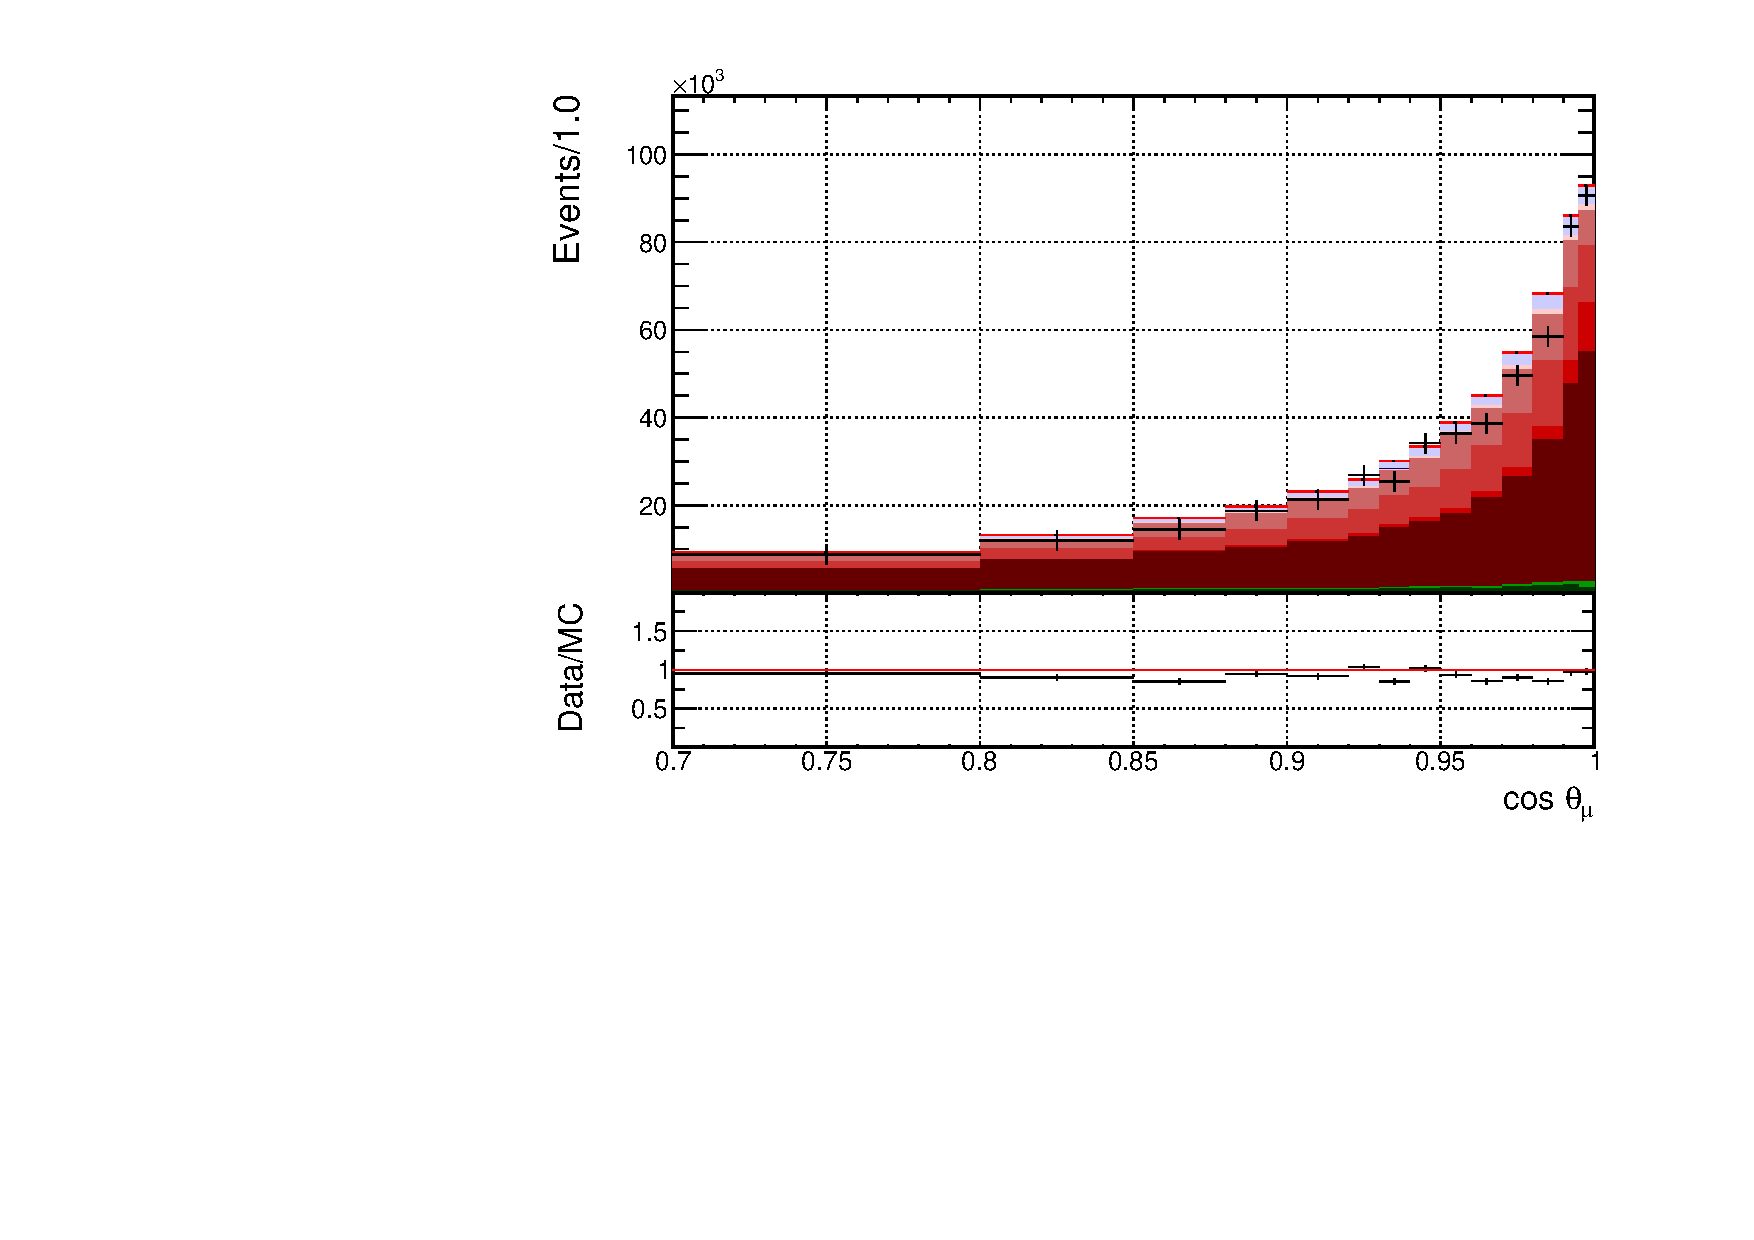
\includegraphics[width=0.95\linewidth]{figs/FGD1_numuCC_1pi_t}
  \caption{FGD1 FHC $\nu_{\mu}$ 1$\pi$}
  \label{fig:tstack_FGD1_numuCC_1pi}
\end{subfigure}
\begin{subfigure}{.32\textwidth}
  \centering
  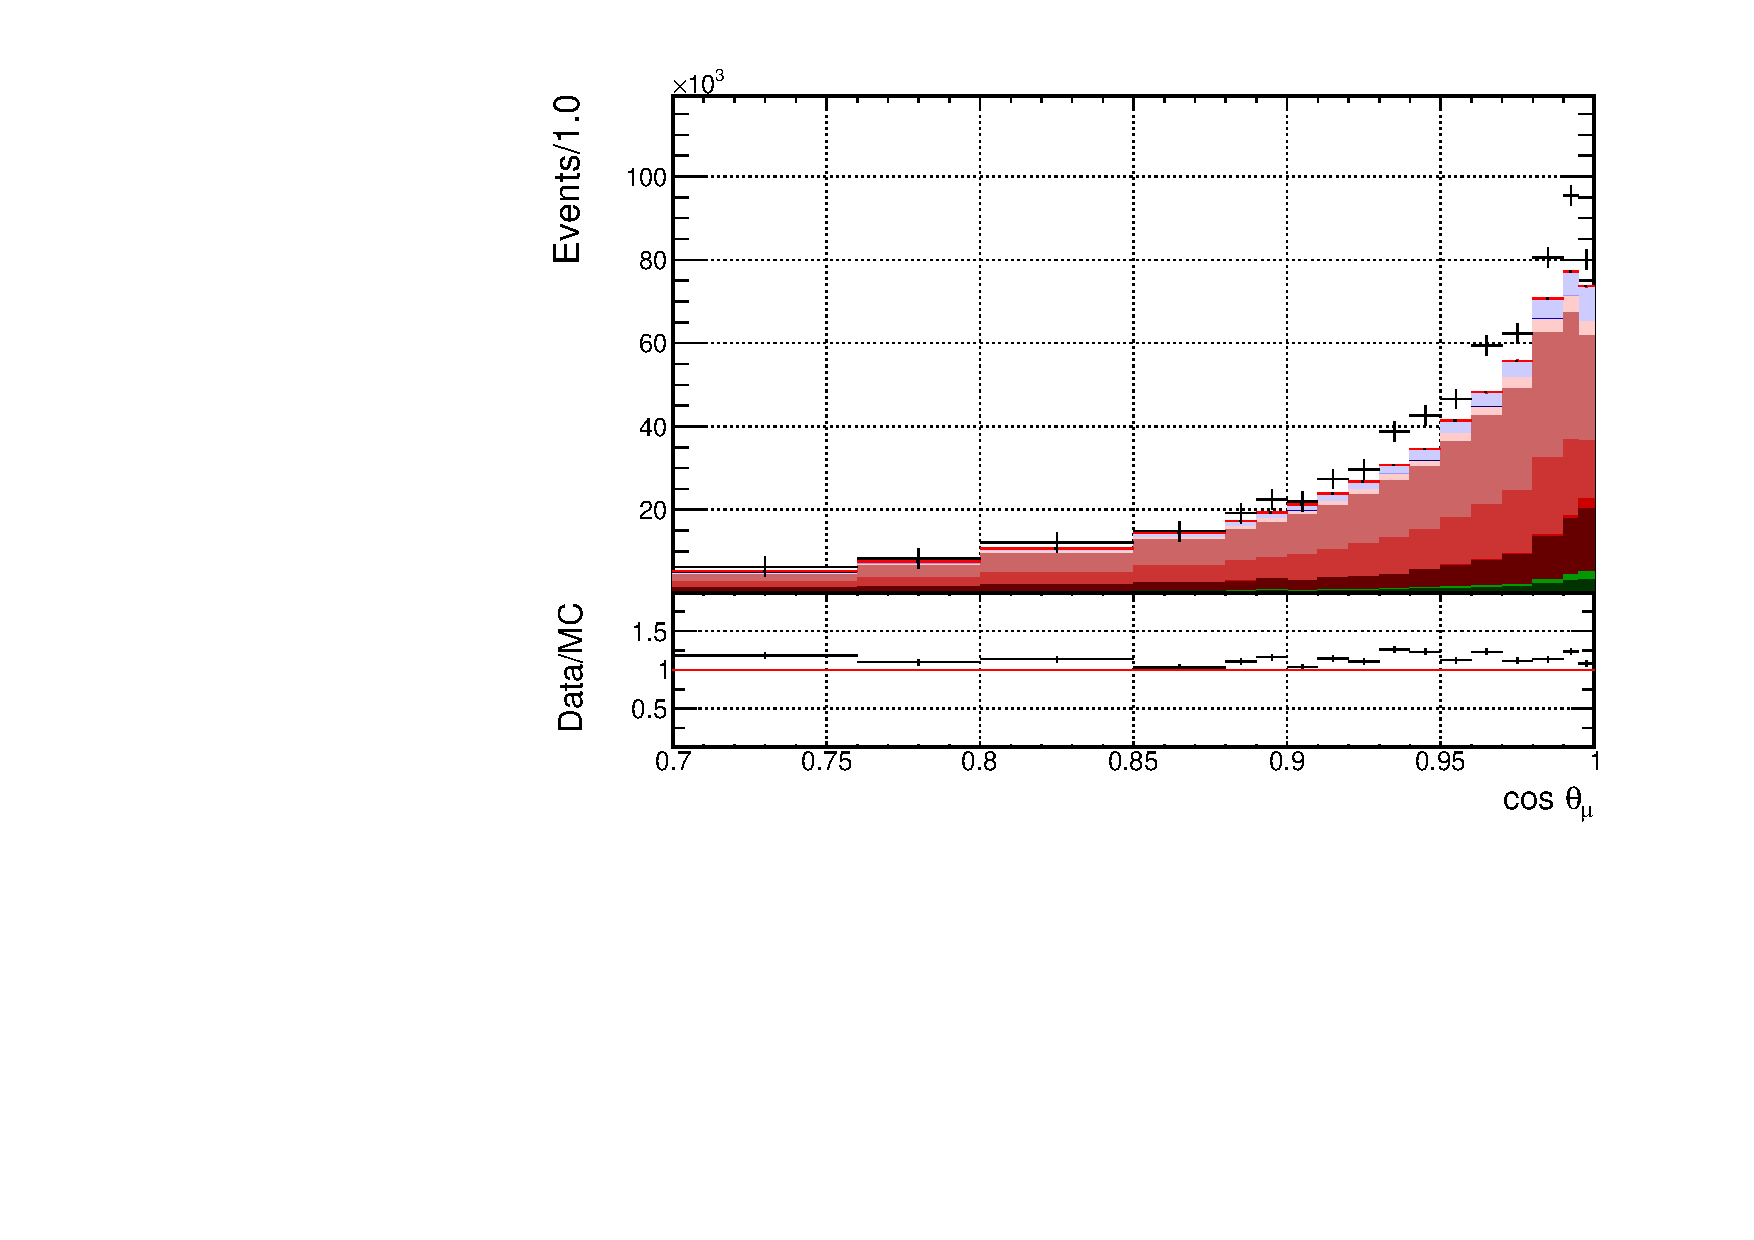
\includegraphics[width=0.95\linewidth]{figs/FGD1_numuCC_other_t}
  \caption{FGD1 FHC $\nu_{\mu}$ Other}
  \label{fig:tstack_FGD1_numuCC_other}
\end{subfigure}
\centering
\begin{subfigure}{.32\textwidth}
  \centering
  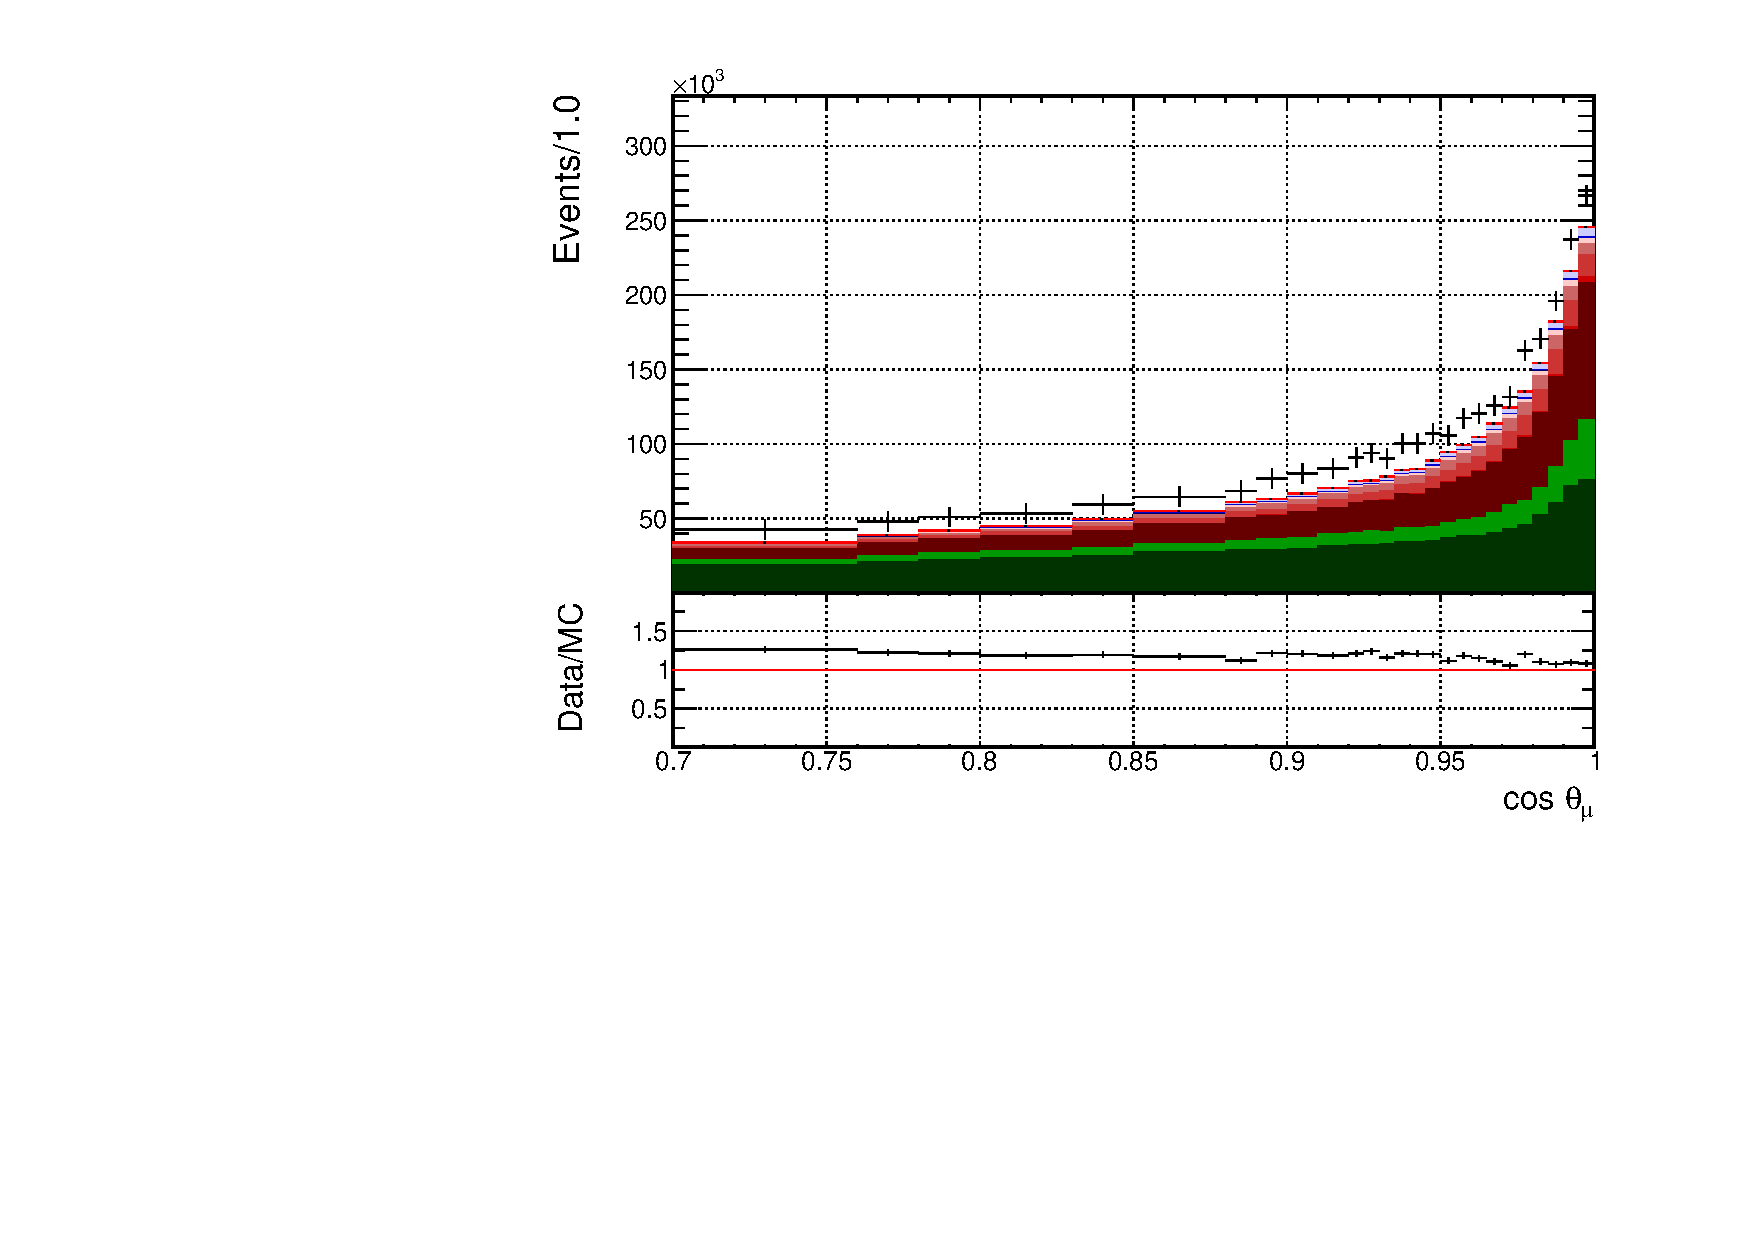
\includegraphics[width=0.95\linewidth]{figs/FGD2_numuCC_0pi_t}
  \caption{FGD2 FHC $\nu_{\mu}$ 0$\pi$}
  \label{fig:tstack_FGD2_numuCC_0pi}
\end{subfigure}
\begin{subfigure}{.32\textwidth}
  \centering
  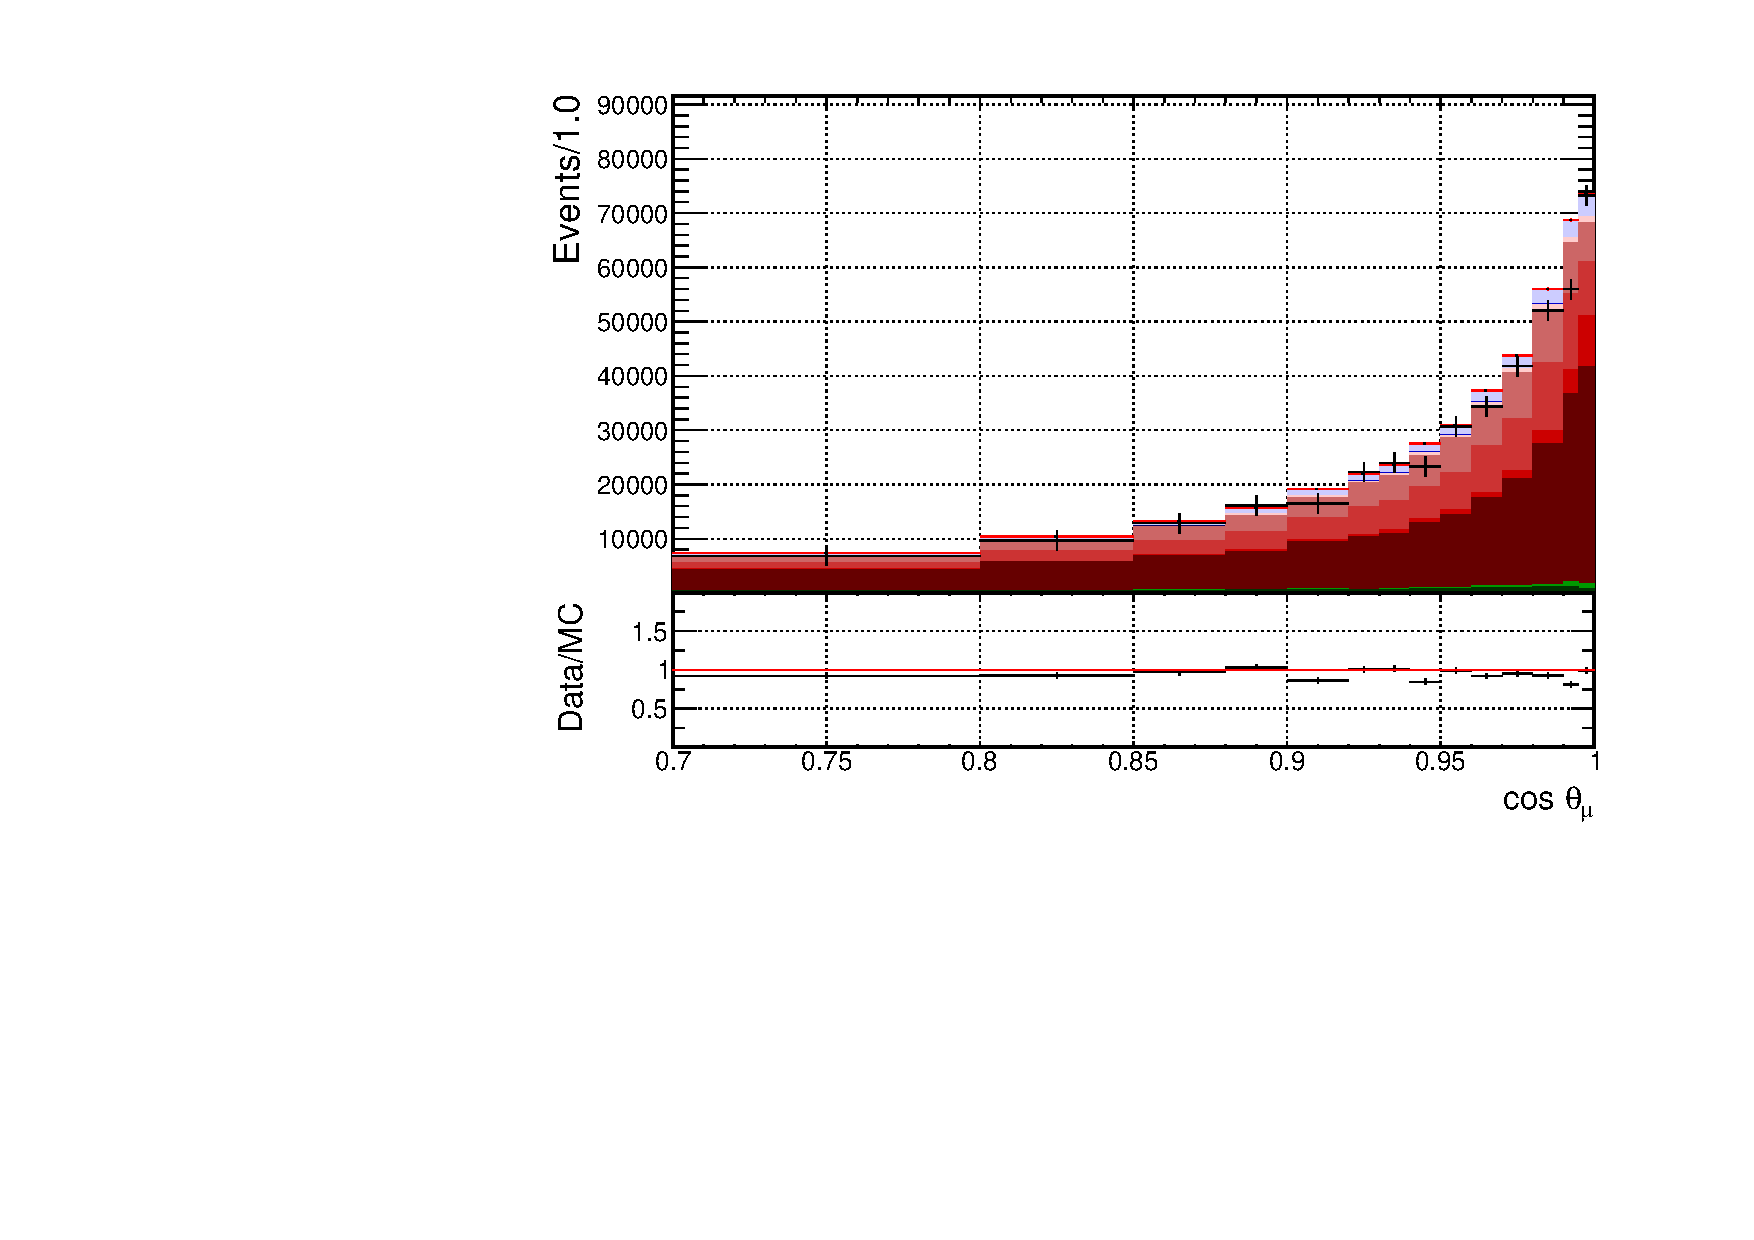
\includegraphics[width=0.95\linewidth]{figs/FGD2_numuCC_1pi_t}
  \caption{FGD2 FHC $\nu_{\mu}$ 1$\pi$}
  \label{fig:tstack_FGD2_numuCC_1pi}
\end{subfigure}
\begin{subfigure}{.32\textwidth}
  \centering
  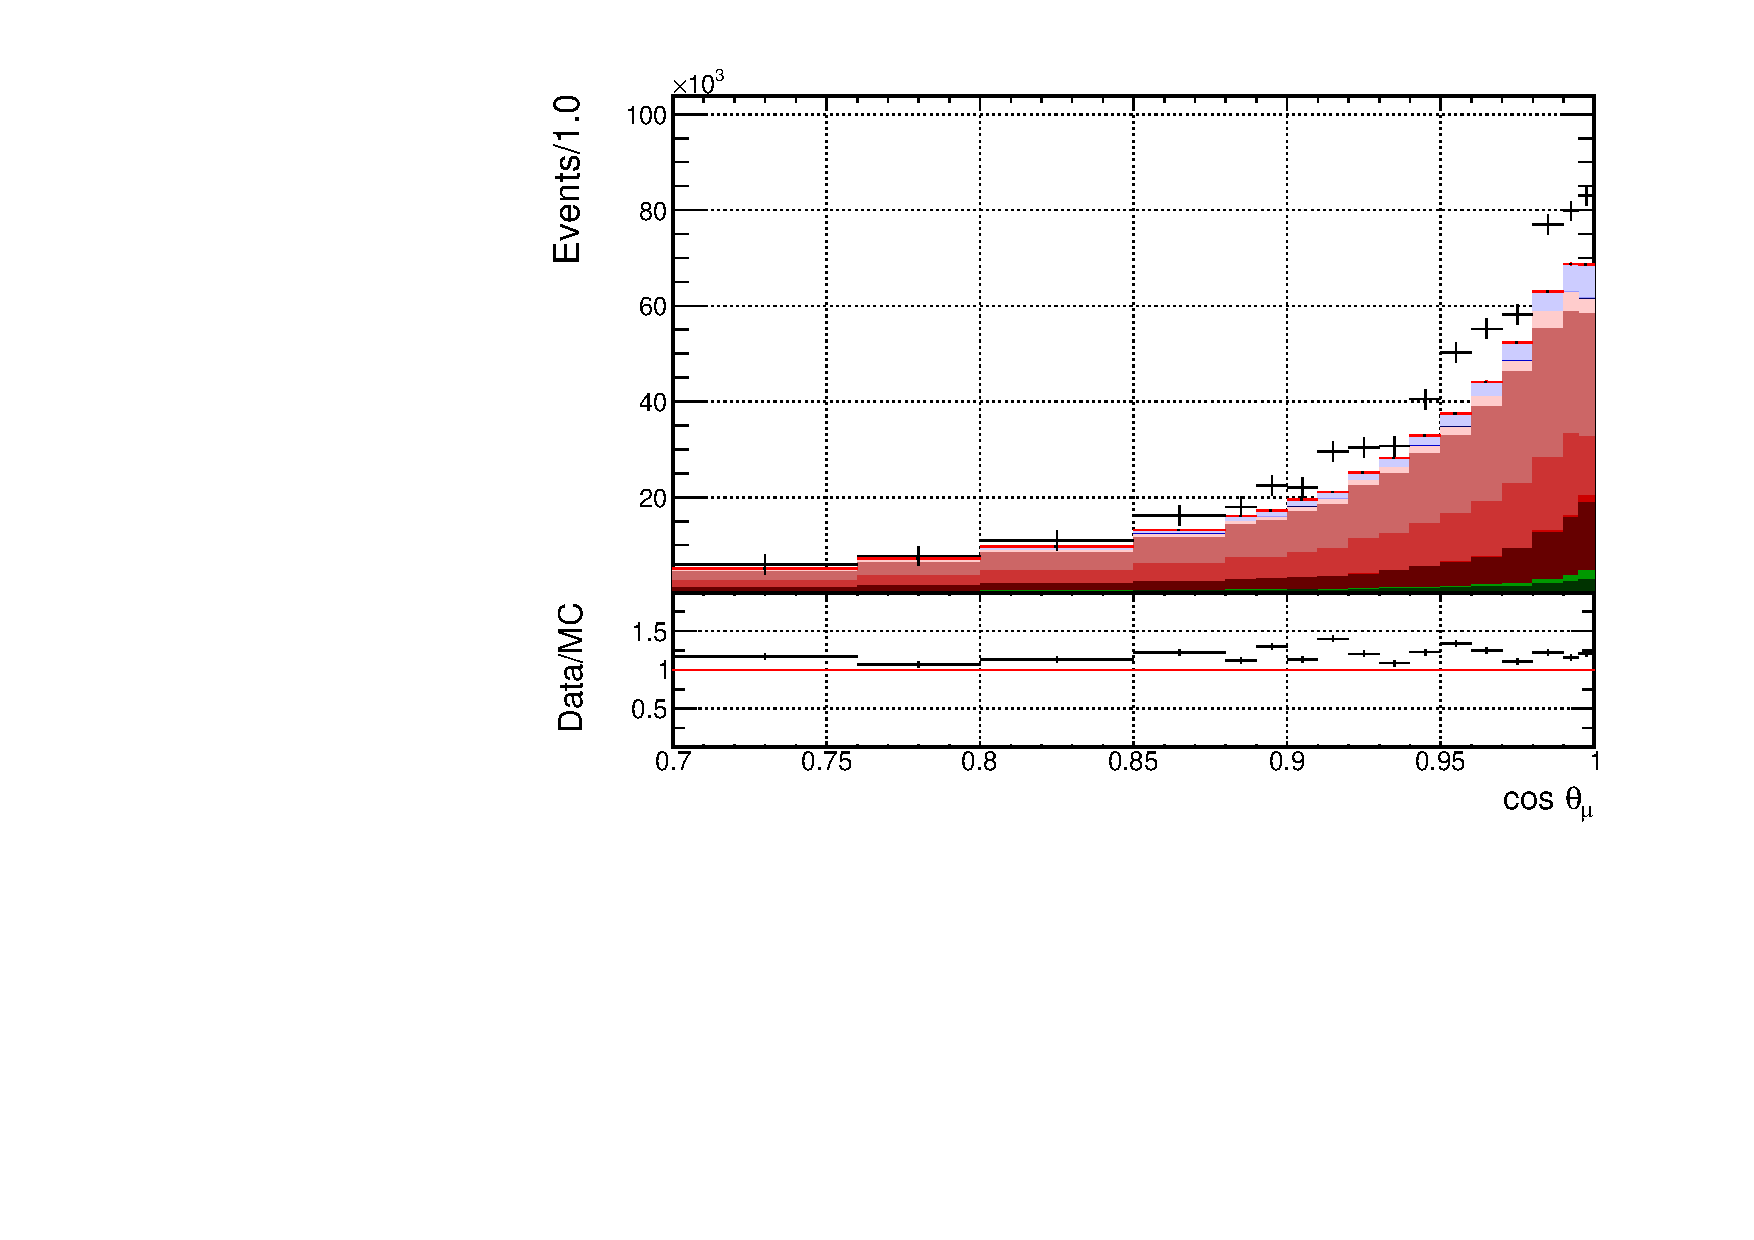
\includegraphics[width=0.95\linewidth]{figs/FGD2_numuCC_other_t}
  \caption{FGD2 FHC $\nu_{\mu}$ Other}
  \label{fig:tstack_FGD2_numuCC_other}
\end{subfigure}
\centering
\begin{subfigure}{.32\textwidth}
  \centering
  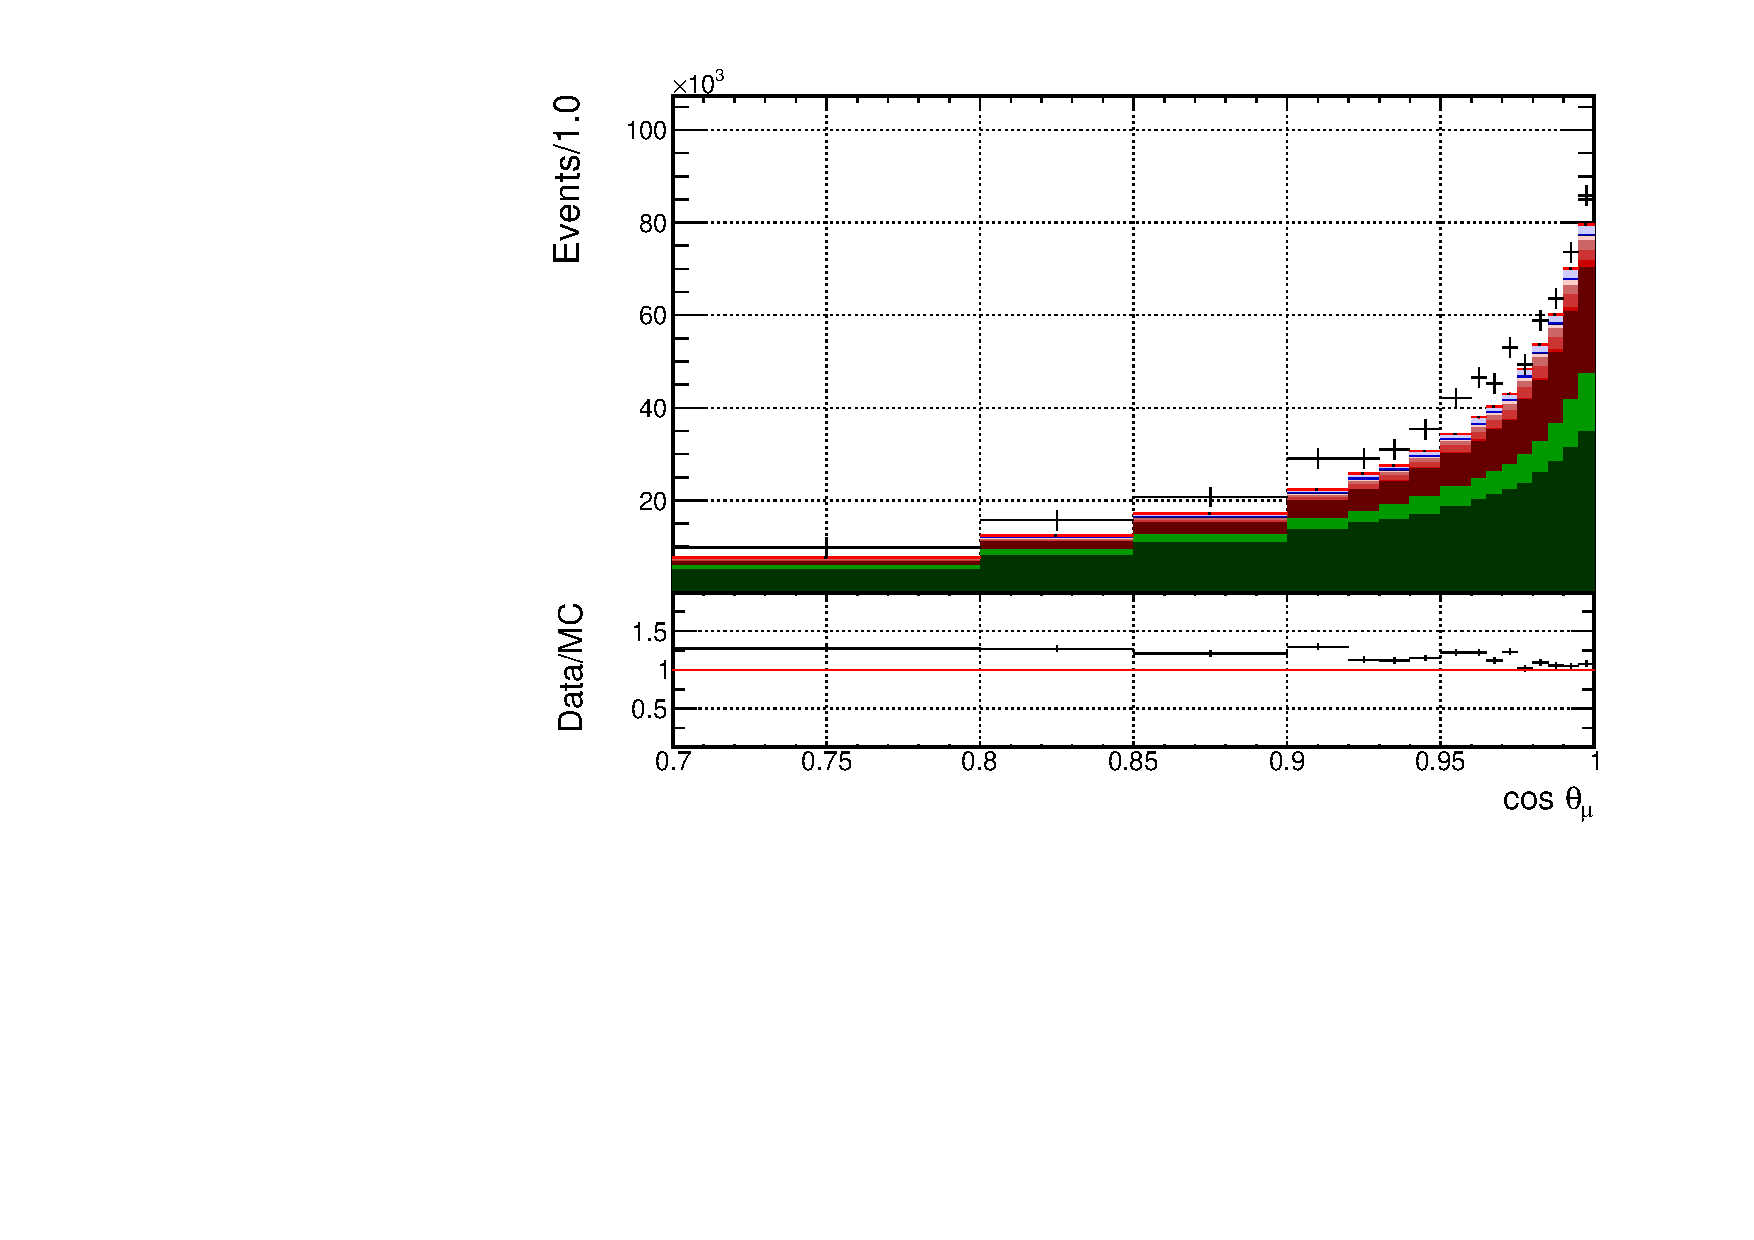
\includegraphics[width=0.95\linewidth]{figs/FGD1_anti-numuCC_0pi_t}
  \caption{FGD1 RHC $\bar{\nu_{\mu}}$ 0$\pi$}
  \label{fig:tstack_FGD1_anti-numuCC_0pi}
\end{subfigure}
\begin{subfigure}{.32\textwidth}
  \centering
  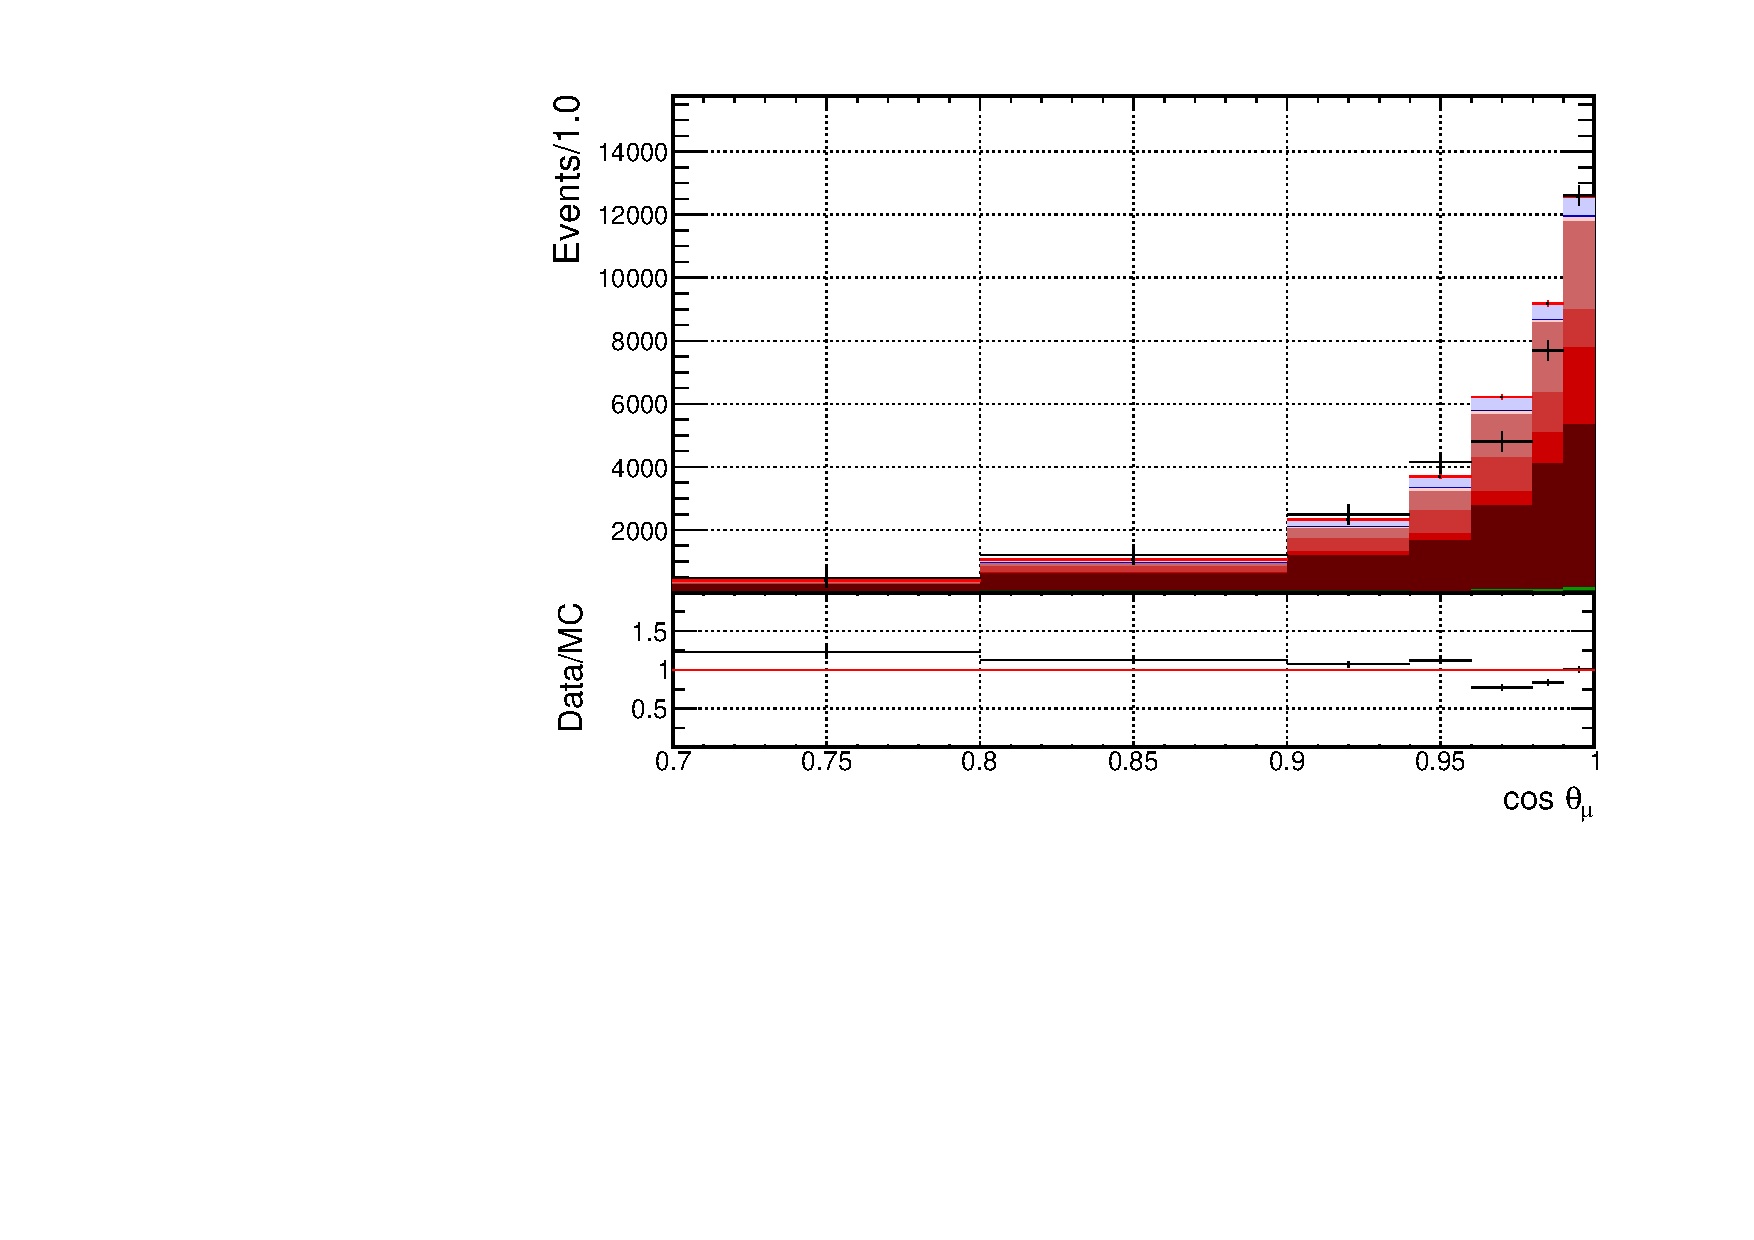
\includegraphics[width=0.95\linewidth]{figs/FGD1_anti-numuCC_1pi_t}
  \caption{FGD1 RHC $\bar{\nu_{\mu}}$ 1$\pi$}
  \label{fig:tstack_FGD1_anti-numuCC_1pi}
\end{subfigure}
\begin{subfigure}{.32\textwidth}
  \centering
  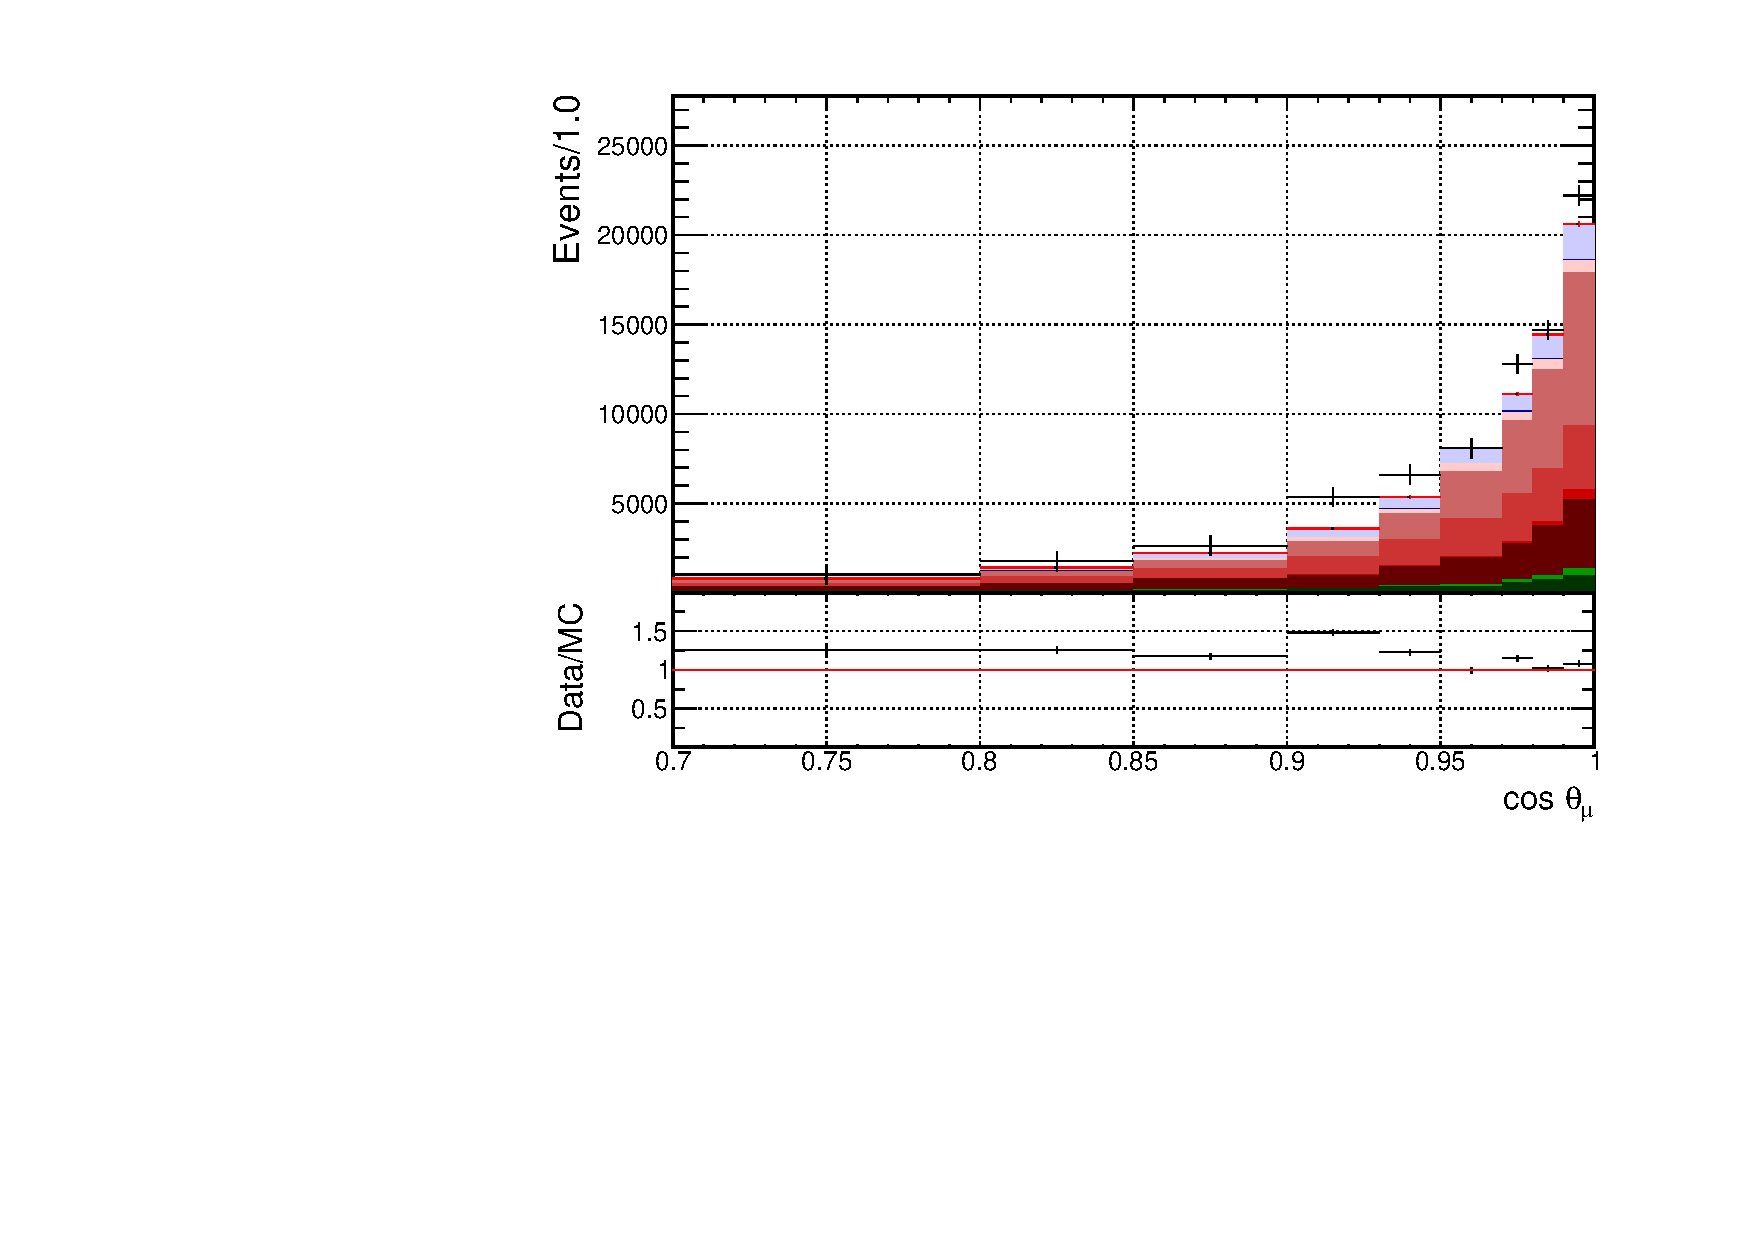
\includegraphics[width=0.95\linewidth]{figs/FGD1_anti-numuCC_other_t}
  \caption{FGD1 RHC $\bar{\nu_{\mu}}$ Other}
  \label{fig:tstack_FGD1_anti-numuCC_other}
\end{subfigure}
\centering
\begin{subfigure}{.32\textwidth}
  \centering
  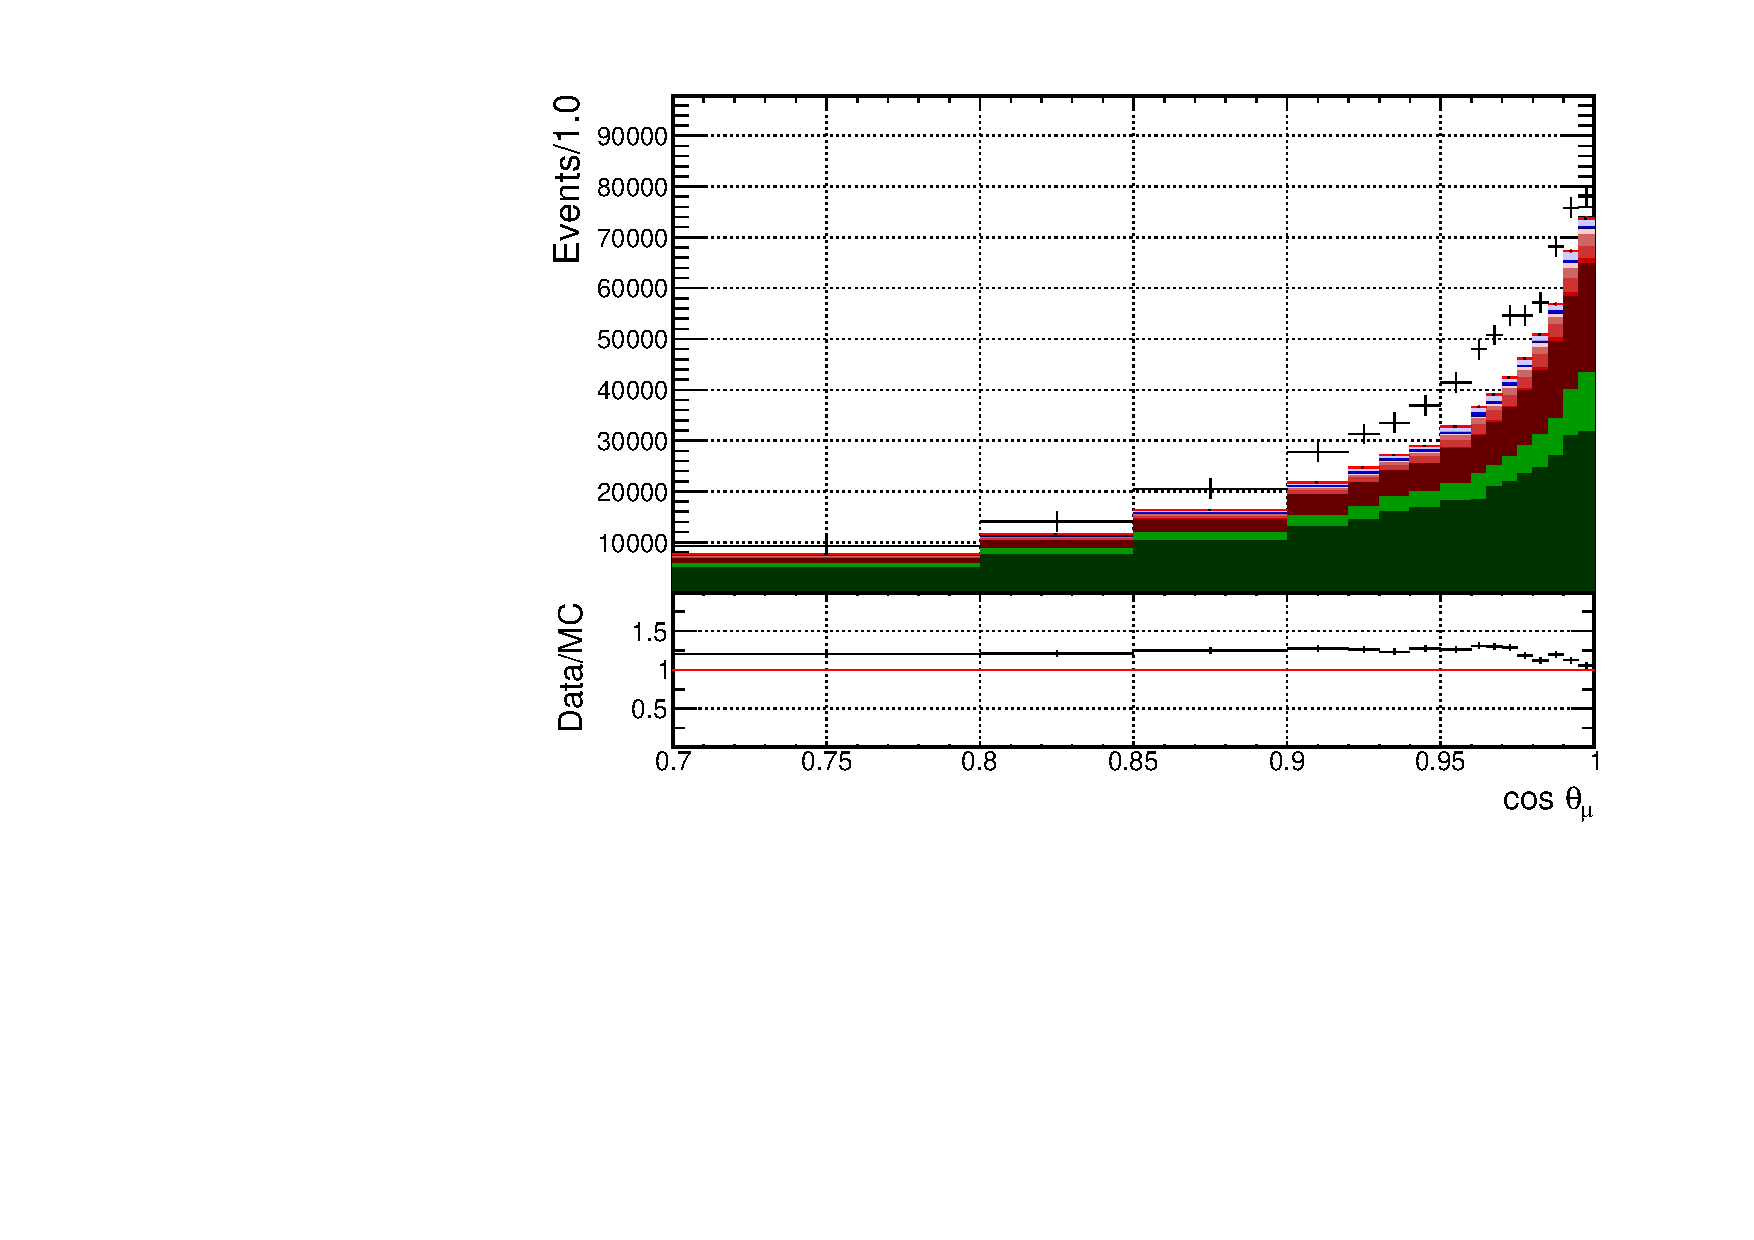
\includegraphics[width=0.95\linewidth]{figs/FGD2_anti-numuCC_0pi_t}
  \caption{FGD2 RHC $\bar{\nu_{\mu}}$ 0$\pi$}
  \label{fig:tstack_FGD2_anti-numuCC_0pi}
\end{subfigure}
\begin{subfigure}{.32\textwidth}
  \centering
  \includegraphics[width=0.95\linewidth]{figs/FGD2_anti-numuCC_1pi_t}
  \caption{FGD2 RHC $\bar{\nu_{\mu}}$ 1$\pi$}
  \label{fig:tstack_FGD2_anti-numuCC_1pi}
\end{subfigure}
\begin{subfigure}{.32\textwidth}
  \centering
  \includegraphics[width=0.95\linewidth]{figs/FGD2_anti-numuCC_other_t}
  \caption{FGD2 RHC $\bar{\nu_{\mu}}$ Other}
  \label{fig:tstack_FGD2_anti-numuCC_other}
\end{subfigure}
\begin{subfigure}{.32\textwidth}
  \centering
  \includegraphics[width=0.95\linewidth]{figs/FGD1_NuMuBkg_CC0pi_in_AntiNu_Mode_t}
  \caption{FGD1 RHC $\nu_{\mu}$ 0$\pi$}
  \label{fig:tstack_FGD1_NuMuBkg_CC0pi_in_AntiNu_Mode}
\end{subfigure}
\begin{subfigure}{.32\textwidth}
  \centering
  \includegraphics[width=0.95\linewidth]{figs/FGD1_NuMuBkg_CC1pi_in_AntiNu_Mode_t}
  \caption{FGD1 RHC $\nu_{\mu}$ 1$\pi$}
  \label{fig:tstack_FGD1_NuMuBkg_CC1pi_in_AntiNu_Mode}
\end{subfigure}
\begin{subfigure}{.32\textwidth}
  \centering
  \includegraphics[width=0.95\linewidth]{figs/FGD1_NuMuBkg_CCOther_in_AntiNu_Mode_t}
  \caption{FGD1 RHC $\nu_{\mu}$ Other}
  \label{fig:tstack_FGD1_NuMuBkg_CCOther_in_AntiNu_Mode}
\end{subfigure}
\begin{subfigure}{.32\textwidth}
  \centering
  \includegraphics[width=0.95\linewidth]{figs/FGD2_NuMuBkg_CC0pi_in_AntiNu_Mode_t}
  \caption{FGD2 RHC $\nu_{\mu}$ 0$\pi$}
  \label{fig:tstack_FGD2_NuMuBkg_CC0pi_in_AntiNu_Mode}
\end{subfigure}
\begin{subfigure}{.32\textwidth}
  \centering
  \includegraphics[width=0.95\linewidth]{figs/FGD2_NuMuBkg_CC1pi_in_AntiNu_Mode_t}
  \caption{FGD2 RHC $\nu_{\mu}$ 1$\pi$}
  \label{fig:tstack_FGD2_NuMuBkg_CC1pi_in_AntiNu_Mode}
\end{subfigure}
\begin{subfigure}{.32\textwidth}
  \centering
  \includegraphics[width=0.95\linewidth]{figs/FGD2_NuMuBkg_CCOther_in_AntiNu_Mode_t}
  \caption{FGD2 RHC $\nu_{\mu}$ Other}
  \label{fig:tstack_FGD2_NuMuBkg_CCOther_in_AntiNu_Mode}
\end{subfigure}
\caption{cos $\theta_{\mu}$ projections of data and nominal MC broken down by interaction mode.}
\label{fig:tstack}
\end{figure}

\section{Log-likelihood Scans}\label{sec:llhscan}

As described in Section \ref{sec:extrac}, the marginalisation effects from extracting correlated and non-Gaussian parameters from the full posterior distribution can cause the fit to appear biased. A full Asimov fit alone, described in Section \ref{sec:asimov}, is therefore not a good method of validating the framework. log-likelihood scans are therefore also run as part of the validations. The nominal MC is set as the data, and each systematic parameter is varied one at a time to 150 equally spaced points from -1$\sigma$ to +1$\sigma$. At each step, the MC is reweighted and the total likelihood from all contributions calculated. Only the diagonal terms of the covariance matrices are used for the penalty contribution, as otherwise varying one parameter alone could invoke significant penalties from correlations. The scans are therefore not a fully accurate measure of the sensitivity of the fit to constrain each systematic, but a useful validation of the framework.

After each scan, the parameter is reset, and the next parameter in question varied. The likelihood response is expected to be fairly Gaussian for each parameter, as the prior uncertainty is either Gaussian or flat, and most parameters are expected to have a symmetric effect on the number of events in individual bins. The minimum should be at the prior central value of the parameter, and the log-likelihood here should be 0, as at this point the reweighted MC is identical to the nominal MC. No variation of a single parameter should be able to produce a set of distributions more similar to the nominal MC than itself.

The log-likelihood scans for four selected interaction parameters are shown in Figure \ref{fig:llhxsec}. As expected, the test statistic minimises to 0 at the prior central value of each parameter. The penalty contribution to the log-likelihood dominates for the CC normalisation parameter, due to the prior uncertainty being so small. Conversely, the 2p2h $^{12}C$ to $^{16}O$ normalisation parameter has a weaker prior and therefore a larger contribution from the sample likelihood. The likelihood for the $0.0 < Q^2 < 0.05$ GeV$^2$ normalisation parameter is entirely dominated by the sample contribution, as the prior is flat. The CC DIS and mult-$\pi$ $\bar{\nu}$ normalisation parameter has more balanced contributions from both the sample and penalty likelihoods.

\begin{figure}
\centering
\begin{subfigure}{.49\textwidth}
  \centering
  \includegraphics[width=0.7\linewidth]{figs/llh/CC_norm_nu_llh.pdf}
  \caption{CC normalisation $\nu$}
\end{subfigure}
\begin{subfigure}{.49\textwidth}
  \centering
  \includegraphics[width=0.7\linewidth]{figs/llh/2p2h_normCtoO_llh.pdf}
  \caption{2p2h $^{12}C$ to $^{16}O$ normalisation}
\end{subfigure}
\begin{subfigure}{.49\textwidth}
  \centering
  \includegraphics[width=0.7\linewidth]{figs/llh/Q2_norm_1_llh.pdf}
  \caption{$0.0 < Q^2 < 0.05$ normalisation}
\end{subfigure}
\begin{subfigure}{.49\textwidth}
  \centering
  \includegraphics[width=0.7\linewidth]{figs/llh/CC_DIS_MultPi_Norm_Nubar_llh.pdf}
  \caption{CC DIS and mult-$\pi$ normalisation}
\end{subfigure}
\caption{log-likelihood scans for selected interaction parameters.}
\label{fig:llhxsec}
\end{figure}

The log-likelihood scans for four selected flux parameters are shown in Figure \ref{fig:llhflux}. The test statistic again minimises to 0 at the prior central value of each parameter, as expected. These parameters all have tight prior uncertainties, and so the penalty terms dominate the likelihoods. For the SK flux parameters, there is no sample contribution to the likelihood. This is expected as the SK flux parameters should have no effect on the ND280 samples (apart from through the correlations with ND280 flux parameters, which are not included in these scans). 

\begin{figure}
\centering
\begin{subfigure}{.49\textwidth}
  \centering
  \includegraphics[width=0.7\linewidth]{figs/llh/b_5_llh.pdf}
  \caption{ND280 FHC $\nu_{\mu}$ 1-1.5 GeV}
\end{subfigure}
\begin{subfigure}{.49\textwidth}
  \centering
  \includegraphics[width=0.7\linewidth]{figs/llh/b_12_llh.pdf}
  \caption{ND280 FHC $\nu_{e}$ 0.5-0.7 GeV}
\end{subfigure}
\begin{subfigure}{.49\textwidth}
  \centering
  \includegraphics[width=0.7\linewidth]{figs/llh/b_36_llh.pdf}
  \caption{ND280 RHC $\nu_e$ 2.5-30 GeV}
\end{subfigure}
\begin{subfigure}{.49\textwidth}
  \centering
  \includegraphics[width=0.7\linewidth]{figs/llh/b_52_llh.pdf}
  \caption{SK RHC $\bar{\nu_{\mu}}$ 0.5-0.6 GeV}
\end{subfigure}
\caption{log-likelihood scans for selected flux parameters.}
\label{fig:llhflux}
\end{figure}

The log-likelihood scans for four selected ND280 detector parameters are shown in Figure \ref{fig:llhdet}. As expected, the test statistics all minimise to 0 at the prior central value of each parameter. The prior dominates for all regions of $p_{\mu}$-cos $\theta_{\mu}$ in each sample. For the higher statistic regions (eg. FGD1 FHC $\nu_{\mu}$ CC 0$\pi$: 300-1000 MeV, 0.92-0.98), the overall constraint is larger than for the lower statistic regions, (eg. FGD1 FHC $\nu_{\mu}$ CC 1$\pi$: 5000-30000 MeV, -1.0-0.6). 

\begin{figure}
\centering
\begin{subfigure}{.49\textwidth}
  \centering
  \includegraphics[width=0.7\linewidth]{figs/llh/ndd_13_llh.pdf}
  \caption{FGD1 FHC $\nu_{\mu}$ CC 0$\pi$: 300-1000 MeV, 0.92-0.98}
\end{subfigure}
\begin{subfigure}{.49\textwidth}
  \centering
  \includegraphics[width=0.7\linewidth]{figs/llh/ndd_136_llh.pdf}
  \caption{FGD1 FHC $\nu_{\mu}$ CC 1$\pi$: 5000-30000 MeV, -1.0-0.6}
\end{subfigure}
\begin{subfigure}{.49\textwidth}
  \centering
  \includegraphics[width=0.7\linewidth]{figs/llh/ndd_541_llh.pdf}
  \caption{FGD2 RHC $\bar{\nu_{\mu}}$ CC Other: 800-30000 MeV, 0.97-1.0}
\end{subfigure}
\begin{subfigure}{.49\textwidth}
  \centering
  \includegraphics[width=0.7\linewidth]{figs/llh/ndd_556_llh.pdf}
  \caption{FGD1 RHC $\nu_{\mu}$ CC Other: 600-30000 MeV, -1.0-0.7}
\end{subfigure}
\caption{log-likelihood scans for selected ND280 detector parameters.}
\label{fig:llhdet}
\end{figure}

\section{Parameter Variations}\label{sec:sigvar}

As a further validation of the fitting framework and models, the parameters are again each set to $\pm1\sigma$, one by one, while all others are held at nominal. Instead of the change in likelihood, here the effect on the event distributions in $p_{\mu}$-cos$\theta_{\mu}$ is inspected. 

One varied interaction parameter for each sample is shown in Figure \ref{fig:sigvars}. The combinations of parameter and sample were selected such that the parameter controls interactions targeted by the sample. The parameter in question is set to $+1\sigma$ above its nominal value, and the ratio of the nominal MC to the reweighted MC is taken.

\begin{figure}
\centering
\begin{subfigure}{.32\textwidth}
  \centering
  \includegraphics[width=0.85\linewidth]{figs/sig/FGD1_numuCC_0pi_2p2h_norm_nu_+1sig.pdf}
  \caption{FGD1 FHC $\nu_{\mu}$ 0$\pi$: 2p2h Norm. $\nu$ += $1\sigma$}
  \label{fig:sigvar_FGD1_numuCC_0pi}
\end{subfigure}
\begin{subfigure}{.32\textwidth}
  \centering
  \includegraphics[width=0.85\linewidth]{figs/sig/FGD1_numuCC_1pi_FEFQEH_+1sig.pdf}
  \caption{FGD1 FHC $\nu_{\mu}$ 1$\pi$: $\pi$ FSI QE High E += $1\sigma$}
  \label{fig:sigvar_FGD1_numuCC_1pi}
\end{subfigure}
\begin{subfigure}{.32\textwidth}
  \centering
  \includegraphics[width=0.85\linewidth]{figs/sig/FGD1_numuCC_other_CC_AGKY_Mult_+1sig.pdf}
  \caption{FGD1 FHC $\nu_{\mu}$ Other: CC AGKY Mult. += $1\sigma$}
  \label{fig:sigvar_FGD1_numuCC_other}
\end{subfigure}
\centering
\begin{subfigure}{.32\textwidth}
  \centering
  \includegraphics[width=0.85\linewidth]{figs/sig/FGD2_numuCC_0pi_Q2_norm_7_+1sig.pdf}
  \caption{FGD2 FHC $\nu_{\mu}$ 0$\pi$: $Q^2 > 1.0$ GeV$^2$ += $1\sigma$}
  \label{fig:sigvar_FGD2_numuCC_0pi}
\end{subfigure}
\begin{subfigure}{.32\textwidth}
  \centering
  \includegraphics[width=0.85\linewidth]{figs/sig/FGD2_numuCC_1pi_CA5_+1sig.pdf}
  \caption{FGD2 FHC $\nu_{\mu}$ 1$\pi$: CA5 += $1\sigma$}
  \label{fig:sigvar_FGD2_numuCC_1pi}
\end{subfigure}
\begin{subfigure}{.32\textwidth}
  \centering
  \includegraphics[width=0.85\linewidth]{figs/sig/FGD2_numuCC_other_CC_DIS_MultPi_Norm_Nu_+1sig.pdf}
  \caption{FGD2 FHC $\nu_{\mu}$ Other: DIS/mult $\pi$ Norm. $\nu$ += $1\sigma$}
  \label{fig:sigvar_FGD2_numuCC_other}
\end{subfigure}
\centering
\begin{subfigure}{.32\textwidth}
  \centering
  \includegraphics[width=0.85\linewidth]{figs/sig/FGD1_anti-numuCC_0pi_MAQE_+1sig.pdf}
  \caption{FGD1 RHC $\bar{\nu_{\mu}}$ 0$\pi$: MAQE += $1\sigma$}
  \label{fig:sigvar_FGD1_anti-numuCC_0pi}
\end{subfigure}
\begin{subfigure}{.32\textwidth}
  \centering
  \includegraphics[width=0.85\linewidth]{figs/sig/FGD1_anti-numuCC_1pi_MARES_+1sig.pdf}
  \caption{FGD1 RHC $\bar{\nu_{\mu}}$ 1$\pi$: $M^{RES}_{A}$ += $1\sigma$}
  \label{fig:sigvar_FGD1_anti-numuCC_1pi}
\end{subfigure}
\begin{subfigure}{.32\textwidth}
  \centering
  \includegraphics[width=0.85\linewidth]{figs/sig/FGD1_anti-numuCC_other_CC_BY_DIS_+1sig.pdf}
  \caption{FGD1 RHC $\bar{\nu_{\mu}}$ Other: BY DIS += $1\sigma$}
  \label{fig:sigvar_FGD1_anti-numuCC_other}
\end{subfigure}
\centering
\begin{subfigure}{.32\textwidth}
  \centering
  \includegraphics[width=0.85\linewidth]{figs/sig/FGD2_anti-numuCC_0pi_EB_dial_O_nubar_+1sig.pdf}
  \caption{FGD2 RHC $\bar{\nu_{\mu}}$ 0$\pi$: E$_{b}$ $^{16}O$ $\bar{\nu}$ += $1\sigma$}
  \label{fig:sigvar_FGD2_anti-numuCC_0pi}
\end{subfigure}
\begin{subfigure}{.32\textwidth}
  \centering
  \includegraphics[width=0.85\linewidth]{figs/sig/FGD2_anti-numuCC_1pi_ISO_BKG_+1sig.pdf}
  \caption{FGD2 RHC $\bar{\nu_{\mu}}$ 1$\pi$: $I_{1/2}$ += $1\sigma$}
  \label{fig:sigvar_FGD2_anti-numuCC_1pi}
\end{subfigure}
\begin{subfigure}{.32\textwidth}
  \centering
  \includegraphics[width=0.85\linewidth]{figs/sig/FGD2_anti-numuCC_other_CC_DIS_MultPi_Norm_Nubar_+1sig.pdf}
  \caption{FGD2 RHC $\bar{\nu_{\mu}}$ Other: DIS/mult-$\pi$ Norm. $\bar{\nu}$ += $1\sigma$}
  \label{fig:sigvar_FGD2_anti-numuCC_other}
\end{subfigure}
\begin{subfigure}{.32\textwidth}
  \centering
  \includegraphics[width=0.85\linewidth]{figs/sig/FGD1_NuMuBkg_CC0pi_in_AntiNu_Mode_2p2h_shape_C_+1sig.pdf}
  \caption{FGD1 RHC $\nu_{\mu}$ 0$\pi$: 2p2h Shape $^{12}C$ += $1\sigma$}
  \label{fig:sigvar_FGD1_NuMuBkg_CC0pi_in_AntiNu_Mode}
\end{subfigure}
\begin{subfigure}{.32\textwidth}
  \centering
  \includegraphics[width=0.85\linewidth]{figs/sig/FGD1_NuMuBkg_CC1pi_in_AntiNu_Mode_CC_Coh_C_+1sig.pdf}
  \caption{FGD1 RHC $\nu_{\mu}$ 1$\pi$: CC Coh $^{12}C$ += $1\sigma$}
  \label{fig:sigvar_FGD1_NuMuBkg_CC1pi_in_AntiNu_Mode}
\end{subfigure}
\begin{subfigure}{.32\textwidth}
  \centering
  \includegraphics[width=0.85\linewidth]{figs/sig/FGD1_NuMuBkg_CCOther_in_AntiNu_Mode_CC_Misc_+1sig.pdf}
  \caption{FGD1 RHC $\nu_{\mu}$ Other: CC Misc. += $1\sigma$}
  \label{fig:sigvar_FGD1_NuMuBkg_CCOther_in_AntiNu_Mode}
\end{subfigure}
\begin{subfigure}{.32\textwidth}
  \centering
  \includegraphics[width=0.85\linewidth]{figs/sig/FGD2_NuMuBkg_CC0pi_in_AntiNu_Mode_Q2_norm_0_+1sig.pdf}
  \caption{FGD2 RHC $\nu_{\mu}$ 0$\pi$: $0.00 < Q^2 < 0.05$ GeV$^2$ += $1\sigma$}
  \label{fig:sigvar_FGD2_NuMuBkg_CC0pi_in_AntiNu_Mode}
\end{subfigure}
\begin{subfigure}{.32\textwidth}
  \centering
  \includegraphics[width=0.85\linewidth]{figs/sig/FGD2_NuMuBkg_CC1pi_in_AntiNu_Mode_FEFABS_+1sig.pdf}
  \caption{FGD2 RHC $\nu_{\mu}$ 1$\pi$: $\pi$ FSI Abs += $1\sigma$}
  \label{fig:sigvar_FGD2_NuMuBkg_CC1pi_in_AntiNu_Mode}
\end{subfigure}
\begin{subfigure}{.32\textwidth}
  \centering
  \includegraphics[width=0.85\linewidth]{figs/sig/FGD2_NuMuBkg_CCOther_in_AntiNu_Mode_CC_BY_MPi_+1sig.pdf}
  \caption{FGD2 RHC $\nu_{\mu}$ Other: BY mult-$\pi$ += $1\sigma$}
  \label{fig:sigvar_FGD2_NuMuBkg_CCOther_in_AntiNu_Mode}
\end{subfigure}
\caption{Ratio of each sample to nominal with one parameter set to $+1\sigma$. The  selected parameters shown all affect events which the sample they're shown for target.}
\label{fig:sigvars}
\end{figure}

The 2p2h $\nu$ normalisation, $Q^2$ normalisations, and $M^{QE}_A$ parameters all have a $Q^2$ dependence in the response of event distributions when set to $+1\sigma$. $M^{QE}_A$ and $Q^{2}>1.0$ GeV$^2$ have a larger effect at high Q$^2$, while the $0.00<Q^{2}<0.05$ GeV$^2$ controls the lower Q$^2$ region, as would be expected.

The $\pi$ FSI, and 2p2h Shape $^{12}C$ parameters reduce the number of events in the shown samples, despite being set higher than nominal. This is because as they are not normalisation parameters, the weight applied can be lower for a higher parameter value. The AGKY mult-$\pi$, C$^{A}_{5}$, $M^{RES}_{A}$, BY DIS, BY mult-$\pi$, and $I_{1/2}$ uncertainties are all shape parameters which cause an increase in events in the samples shown when set to $+1\sigma$. E$_{b}$ $^{16}O$ $\bar{\nu}$ causes an increase in events at low momentum, and decrease at higher momentum, as the events are directly shifted and not just reweighted.

The DIS normalisations, CC coh $^{16}O$, and CC Misc. normalisations all increase events at high angle when set to $+1\sigma$. The DIS normalisations effect higher momentum events, as would be expected as DIS events tend to involve higher energies. The CC Misc. parameter has a large impact despite only affecting a small number of events, because of it's large uncertainty. When it is set to $+1\sigma$ it therefore is significantly higher than at nominal.

All the variations are causing changes to the event distributions in the regions each parameter would be expected to. The total number of events in each sample at each variation is compared between the near detector fitting groups to verify that each parameter is behaving in the same way in each framework.

\section{Asimov Fit}\label{sec:asimov}

For an Asimov fit\footnote{Named after the Isaac Asimov short story, \textit{Franchise}, in which an individual is chosen as the sole voter as their views represent those of the whole population.}, the nominal MC prediction is set to be the `data'. The MC is then fitted to itself. This is completely unphysical, as there can be a non-integer number of `data' events, but means there are no statistical fluctuations in the dataset, and the expected result of the fit is known. Therefore any deviations from the expected result indicate problems with the fitter. The results can also be used to obtain the maximum sensitivity of the fit. The constraint on each parameter shows the reduction in systematic uncertainties that would be achieved if the models perfectly described the true data.

The results of the Asimov fit for the flux parameters are shown in Figure \ref{fig:asmvfluxSK}. As described in Section \ref{sec:stats}, the fit does not find a single best-fit set of parameters, but single parameter values are extracted from the posterior distribution by marginalising over all but one parameter, one by one. Marginalisation effects cause the postfit parameter values to not exactly equal the nominal inputs, but these are very small. The flux parameters with the largest discrepancies are those that apply to rarer events at ND280, such as for high energies, and so are constrained mostly by the prior uncertainty only. The constraint on the SK flux parameters comes entirely from the correlation with the ND280 flux parameters, and so the postfit values have the same behaviour.

\begin{figure}
\centering
\begin{subfigure}{0.95\textwidth}
  \centering
  \includegraphics[width=0.24\linewidth]{figs/asmv_leg}
  \caption{}
  \label{fig:}
\end{subfigure}
\begin{subfigure}{0.24\textwidth}
  \centering
  \includegraphics[width=0.95\linewidth]{figs/asmvflux0}
  \caption{ND FHC $\nu_{\mu}$}
  \label{fig:}
\end{subfigure}
\begin{subfigure}{0.24\textwidth}
  \centering
  \includegraphics[width=0.95\linewidth]{figs/asmvflux1}
  \caption{ND FHC $\nu_e$}
  \label{fig:}
\end{subfigure}
\begin{subfigure}{0.24\textwidth}
  \centering
  \includegraphics[width=0.95\linewidth]{figs/asmvflux2}
  \caption{ND FHC $\bar{\nu_{\mu}}$}
  \label{fig:}
\end{subfigure}
\begin{subfigure}{0.24\textwidth}
  \centering
  \includegraphics[width=0.95\linewidth]{figs/asmvflux3}
  \caption{ND FHC $\bar{\nu_{e}}$}
  \label{fig:}
\end{subfigure}
\begin{subfigure}{0.24\textwidth}
  \centering
  \includegraphics[width=0.95\linewidth]{figs/asmvflux4}
  \caption{ND RHC $\bar{\nu_{\mu}}$}
  \label{fig:}
\end{subfigure}
\begin{subfigure}{0.24\textwidth}
  \centering
  \includegraphics[width=0.95\linewidth]{figs/asmvflux5}
  \caption{ND RHC $\bar{\nu_{e}}$}
  \label{fig:}
\end{subfigure}
\begin{subfigure}{0.24\textwidth}
  \centering
  \includegraphics[width=0.95\linewidth]{figs/asmvflux6}
  \caption{ND RHC $\nu_{\mu}$}
  \label{fig:}
\end{subfigure}
\vspace{15mm}
\begin{subfigure}{0.24\textwidth}
  \centering
  \includegraphics[width=0.95\linewidth]{figs/asmvflux7}
  \caption{ND RHC $\nu_e$}
  \label{fig:}
\end{subfigure}
\begin{subfigure}{0.24\textwidth}
  \centering
  \includegraphics[width=0.95\linewidth]{figs/asmvflux8}
  \caption{SK FHC $\nu_{\mu}$}
  \label{fig:}
\end{subfigure}
\begin{subfigure}{0.24\textwidth}
  \centering
  \includegraphics[width=0.95\linewidth]{figs/asmvflux9}
  \caption{SK FHC $\nu_e$}
  \label{fig:}
\end{subfigure}
\begin{subfigure}{0.24\textwidth}
  \centering
  \includegraphics[width=0.95\linewidth]{figs/asmvflux10}
  \caption{SK FHC $\bar{\nu_{\mu}}$}
  \label{fig:}
\end{subfigure}
\begin{subfigure}{0.24\textwidth}
  \centering
  \includegraphics[width=0.95\linewidth]{figs/asmvflux11}
  \caption{SK FHC $\bar{\nu_{e}}$}
  \label{fig:}
\end{subfigure}
\begin{subfigure}{0.24\textwidth}
  \centering
  \includegraphics[width=0.95\linewidth]{figs/asmvflux12}
  \caption{SK RHC $\bar{\nu_{\mu}}$}
  \label{fig:}
\end{subfigure}
\begin{subfigure}{0.24\textwidth}
  \centering
  \includegraphics[width=0.95\linewidth]{figs/asmvflux13}
  \caption{SK RHC $\bar{\nu_e}$}
  \label{fig:}
\end{subfigure}
\begin{subfigure}{0.24\textwidth}
  \centering
  \includegraphics[width=0.95\linewidth]{figs/asmvflux14}
  \caption{SK RHC $\nu_{\mu}$}
  \label{fig:}
\end{subfigure}
\begin{subfigure}{0.24\textwidth}
  \centering
  \includegraphics[width=0.95\linewidth]{figs/asmvflux15}
  \caption{SK RHC $\nu_e$}
  \label{fig:}
\end{subfigure}
\caption{Flux parameters for the Asimov Fit.}
\label{fig:asmvfluxSK}
\end{figure}

The 2p2h energy dependence and low $\pi$ momentum $I_{1/2}$ parameters are not fitted at the near detector so aren't shown here.

The results for the interaction parameters are shown in Figure \ref{fig:asmvxsec}. All parameters stay close to their nominal values, as would be expected. There are several parameters which show small deviations, but these are again parameters which are not well constrained, such as NC 1$\gamma$, as there are few events of the relevant interaction mode at ND280.

\begin{figure}
\centering
\begin{subfigure}{0.95\textwidth}
  \centering
  \includegraphics[width=0.25\linewidth]{figs/asmv_leg}
  \caption{}
  \label{fig:}
\end{subfigure}
\begin{subfigure}{0.49\textwidth}
  \centering
  \includegraphics[width=0.95\linewidth]{figs/asmvxsec1}
  \caption{CC0$\pi$}
  \label{fig:}
\end{subfigure}
\begin{subfigure}{0.49\textwidth}
  \centering
  \includegraphics[width=0.95\linewidth]{figs/asmvxsec2}
  \caption{$Q^2$ and $E_b$}
  \label{fig:}
\end{subfigure}
\begin{subfigure}{0.49\textwidth}
  \centering
  \includegraphics[width=0.95\linewidth]{figs/asmvxsec3}
  \caption{CC1$\pi$, $\nu_e$, CC DIS, CC mult-$\pi$ and CC Coh.}
  \label{fig:}
\end{subfigure}
\begin{subfigure}{0.49\textwidth}
  \centering
  \includegraphics[width=0.95\linewidth]{figs/asmvxsec4}
  \caption{NC}
  \label{fig:}
\end{subfigure}
\begin{subfigure}{0.49\textwidth}
  \centering
  \includegraphics[width=0.95\linewidth]{figs/asmvxsec4}
  \caption{$\pi$ FSI}
  \label{fig:}
\end{subfigure}
\caption{Interaction parameters for the Asimov fit}
\label{fig:asmvxsec}
\end{figure}

The postfit covariance matrix for flux and interaction parameters is shown in Figure \ref{fig:asmvpostfitcov}. There are strong correlations between parameters which control interactions with similar topologies, such as the $M^{QE}_A$, 2p2h, and $Q^2$ parameters. These all affect different regions of $Q^2$, but also all correlate with the flux parameters, causing them to correlate with other. The CC coherent parameters correlate with each other, as do the $\pi$ FSI and single $\pi$ production parameters. The E$_b$ parameters are correlated with each other, and most other parameters. There are also slight correlations between CCQE and CC 1$\pi$ parameters, due to the contamination of CC $1\pi$ events in the CC 0$\pi$ samples. The flux parameters have strong internal correlations from their priors.

\begin{figure}
\centering
\includegraphics*[width=0.9\textwidth,clip]{figs/asmvpostfitcov}
\caption{Asimov postfit covariance matrix for flux and interaction parameters.}\label{fig:asmvpostfitcov}
\end{figure}

\section{Data Fit}\label{sec:datafit}

\subsection{Prior Predictions}

Prior predictions are produced using a similar method to the posterior predictions described in Section \ref{sec:postpred}. However, instead of using draws from the Markov Chain, correlated throws of the fit parameters are made. For each of 2000 throws, the nominal MC is reweighted to the thrown parameter values. Each bin in each sample therefore has 2000 different number of events, from which the central value and uncertainty is used to build the prediction in the same way as for the posterior predictions. This method has the advantage of incorporating the prior uncertainties when inspecting how well the nominal model fits the data, which just looking at the nominal MC does not do. 

The ratio of the prior predictive $p_{\mu}$-cos$\theta_{\mu}$ distributions to data for each sample are shown in Figure \ref{fig:priorpreds}. As expected from comparisons of the nominal MC to data, the prior predictive distributions underestimate the data significantly. If the nominal model perfectly described the data with small uncertainties the fit would not be needed. The prior predictions are compared to the posterior predictions, and data, in Table \ref{}.
\red{update these plots}
\begin{figure}
\centering
\begin{subfigure}{.32\textwidth}
  \centering
  \includegraphics[width=0.85\linewidth]{figs/priorpred_FGD1_numuCC_0pi.pdf}
  \caption{FGD1 FHC $\nu_{\mu}$ 0$\pi$}
  \label{fig:priorpred_FGD1_numuCC_0pi}
\end{subfigure}
\begin{subfigure}{.32\textwidth}
  \centering
  \includegraphics[width=0.85\linewidth]{figs/priorpred_FGD1_numuCC_1pi.pdf}
  \caption{FGD1 FHC $\nu_{\mu}$ 1$\pi$}
  \label{fig:priorpred_FGD1_numuCC_1pi}
\end{subfigure}
\begin{subfigure}{.32\textwidth}
  \centering
  \includegraphics[width=0.85\linewidth]{figs/priorpred_FGD1_numuCC_other.pdf}
  \caption{FGD1 FHC $\nu_{\mu}$ Other}
  \label{fig:priorpred_FGD1_numuCC_other}
\end{subfigure}
\centering
\begin{subfigure}{.32\textwidth}
  \centering
  \includegraphics[width=0.85\linewidth]{figs/priorpred_FGD2_numuCC_0pi.pdf}
  \caption{FGD2 FHC $\nu_{\mu}$ 0$\pi$}
  \label{fig:priorpred_FGD2_numuCC_0pi}
\end{subfigure}
\begin{subfigure}{.32\textwidth}
  \centering
  \includegraphics[width=0.85\linewidth]{figs/priorpred_FGD2_numuCC_1pi.pdf}
  \caption{FGD2 FHC $\nu_{\mu}$ 1$\pi$}
  \label{fig:priorpred_FGD2_numuCC_1pi}
\end{subfigure}
\begin{subfigure}{.32\textwidth}
  \centering
  \includegraphics[width=0.85\linewidth]{figs/priorpred_FGD2_numuCC_other.pdf}
  \caption{FGD2 FHC $\nu_{\mu}$ Other}
  \label{fig:priorpred_FGD2_numuCC_other}
\end{subfigure}
\centering
\begin{subfigure}{.32\textwidth}
  \centering
  \includegraphics[width=0.85\linewidth]{figs/priorpred_FGD1_anti-numuCC_0pi.pdf}
  \caption{FGD1 RHC $\bar{\nu_{\mu}}$ 0$\pi$}
  \label{fig:priorpred_FGD1_anti-numuCC_0pi}
\end{subfigure}
\begin{subfigure}{.32\textwidth}
  \centering
  \includegraphics[width=0.85\linewidth]{figs/priorpred_FGD1_anti-numuCC_1pi.pdf}
  \caption{FGD1 RHC $\bar{\nu_{\mu}}$ 1$\pi$}
  \label{fig:priorpred_FGD1_anti-numuCC_1pi}
\end{subfigure}
\begin{subfigure}{.32\textwidth}
  \centering
  \includegraphics[width=0.85\linewidth]{figs/priorpred_FGD1_anti-numuCC_other.pdf}
  \caption{FGD1 RHC $\bar{\nu_{\mu}}$ Other}
  \label{fig:priorpred_FGD1_anti-numuCC_other}
\end{subfigure}
\centering
\begin{subfigure}{.32\textwidth}
  \centering
  \includegraphics[width=0.85\linewidth]{figs/priorpred_FGD2_anti-numuCC_0pi.pdf}
  \caption{FGD2 RHC $\bar{\nu_{\mu}}$ 0$\pi$}
  \label{fig:priorpred_FGD2_anti-numuCC_0pi}
\end{subfigure}
\begin{subfigure}{.32\textwidth}
  \centering
  \includegraphics[width=0.85\linewidth]{figs/priorpred_FGD2_anti-numuCC_1pi.pdf}
  \caption{FGD2 RHC $\bar{\nu_{\mu}}$ 1$\pi$}
  \label{fig:priorpred_FGD2_anti-numuCC_1pi}
\end{subfigure}
\begin{subfigure}{.32\textwidth}
  \centering
  \includegraphics[width=0.85\linewidth]{figs/priorpred_FGD2_anti-numuCC_other.pdf}
  \caption{FGD2 RHC $\bar{\nu_{\mu}}$ Other}
  \label{fig:priorpred_FGD2_anti-numuCC_other}
\end{subfigure}
\begin{subfigure}{.32\textwidth}
  \centering
  \includegraphics[width=0.85\linewidth]{figs/priorpred_FGD1_NuMuBkg_CC0pi_in_AntiNu_Mode.pdf}
  \caption{FGD1 RHC $\nu_{\mu}$ 0$\pi$}
  \label{fig:priorpred_FGD1_NuMuBkg_CC0pi_in_AntiNu_Mode}
\end{subfigure}
\begin{subfigure}{.32\textwidth}
  \centering
  \includegraphics[width=0.85\linewidth]{figs/priorpred_FGD1_NuMuBkg_CC1pi_in_AntiNu_Mode.pdf}
  \caption{FGD1 RHC $\nu_{\mu}$ 1$\pi$}
  \label{fig:priorpred_FGD1_NuMuBkg_CC1pi_in_AntiNu_Mode}
\end{subfigure}
\begin{subfigure}{.32\textwidth}
  \centering
  \includegraphics[width=0.85\linewidth]{figs/priorpred_FGD1_NuMuBkg_CCOther_in_AntiNu_Mode.pdf}
  \caption{FGD1 RHC $\nu_{\mu}$ Other}
  \label{fig:priorpred_FGD1_NuMuBkg_CCOther_in_AntiNu_Mode}
\end{subfigure}
\begin{subfigure}{.32\textwidth}
  \centering
  \includegraphics[width=0.85\linewidth]{figs/priorpred_FGD2_NuMuBkg_CC0pi_in_AntiNu_Mode.pdf}
  \caption{FGD2 RHC $\nu_{\mu}$ 0$\pi$}
  \label{fig:priorpred_FGD2_NuMuBkg_CC0pi_in_AntiNu_Mode}
\end{subfigure}
\begin{subfigure}{.32\textwidth}
  \centering
  \includegraphics[width=0.85\linewidth]{figs/priorpred_FGD2_NuMuBkg_CC1pi_in_AntiNu_Mode.pdf}
  \caption{FGD2 RHC $\nu_{\mu}$ 1$\pi$}
  \label{fig:priorpred_FGD2_NuMuBkg_CC1pi_in_AntiNu_Mode}
\end{subfigure}
\begin{subfigure}{.32\textwidth}
  \centering
  \includegraphics[width=0.85\linewidth]{figs/priorpred_FGD2_NuMuBkg_CCOther_in_AntiNu_Mode.pdf}
  \caption{FGD2 RHC $\nu_{\mu}$ Other}
  \label{fig:priorpred_FGD2_NuMuBkg_CCOther_in_AntiNu_Mode}
\end{subfigure}
\caption{Ratio to data of the prior predictive distributions.}
\label{fig:priorpreds}
\end{figure}

\subsection{Fit Results}

The MC was then fitted to the real data. The postfit flux parameter values are shown in Figure \ref{fig:datfluxSK}. For the FHC $\nu_{\mu}$ and $\bar{\nu_{\mu}}$, there is a pull of $\sim$10$\%$ below 1 GeV. The pull decreases as the energy decreases, and falls below nominal at higher energies. A similarly high pull is seen for the FHC $\nu_e$ parameters, but this is fairly constant in energy. For the FHC $\bar{\nu_e}$ and RHC $\nu_e$, the pull is $\sim10\%$ for the high energy parameter, but the low energy parameter is close to its nominal value.

The RHC $\bar{\nu_{\mu}}$ parameters are also pulled significantly upwards, to $\sim$15$\%$. The pull oscillates around $\sim$10$\%$ as energy increases. The RHC $\bar{\nu_e}$ parameters oscillate around nominal below 1 GeV, but increase to $\sim$10$\%$ at higher energies. The RHC $\nu_{\mu}$ parameters are pulled to $\sim$10$\%$, but are closer to nominal above 2.5 GeV. Similar behaviour is seen for the ND280 and SK parameters, as would be expected due to their prefit correlations.

Although many of the flux parameters are pulled significantly away from their prior central values, and beyond the prefit $\pm1\sigma$ range, these results are not too concerning. As the flux parameters are so strongly correlated, a pull in one translates to many of them moving. The flux penalty contribution to the log-likelihood at each step in the Markov Chain is shown in Figure \ref{fig:llh_fluxdat}. The stationary distribution is at -2LLH$\approx$50, which for 100 flux parameters corresponds to $\sim1\chi^2$ per degree of freedom.

\begin{figure}
\centering
\begin{subfigure}{0.95\textwidth}
  \centering
  \includegraphics[width=0.24\linewidth]{figs/dat_leg}
  \caption{}
  \label{fig:}
\end{subfigure}
\begin{subfigure}{0.24\textwidth}
  \centering
  \includegraphics[width=0.95\linewidth]{figs/datflux0}
  \caption{ND FHC $\nu_{\mu}$}
  \label{fig:}
\end{subfigure}
\begin{subfigure}{0.24\textwidth}
  \centering
  \includegraphics[width=0.95\linewidth]{figs/datflux1}
  \caption{ND FHC $\nu_e$}
  \label{fig:}
\end{subfigure}
\begin{subfigure}{0.24\textwidth}
  \centering
  \includegraphics[width=0.95\linewidth]{figs/datflux2}
  \caption{ND FHC $\bar{\nu_{\mu}}$}
  \label{fig:}
\end{subfigure}
\begin{subfigure}{0.24\textwidth}
  \centering
  \includegraphics[width=0.95\linewidth]{figs/datflux3}
  \caption{ND FHC $\bar{\nu_{e}}$}
  \label{fig:}
\end{subfigure}
\begin{subfigure}{0.24\textwidth}
  \centering
  \includegraphics[width=0.95\linewidth]{figs/datflux4}
  \caption{ND RHC $\bar{\nu_{\mu}}$}
  \label{fig:}
\end{subfigure}
\begin{subfigure}{0.24\textwidth}
  \centering
  \includegraphics[width=0.95\linewidth]{figs/datflux5}
  \caption{ND RHC $\bar{\nu_{e}}$}
  \label{fig:}
\end{subfigure}
\begin{subfigure}{0.24\textwidth}
  \centering
  \includegraphics[width=0.95\linewidth]{figs/datflux6}
  \caption{ND RHC $\nu_{\mu}$}
  \label{fig:}
\end{subfigure}
\vspace{15mm}
\begin{subfigure}{0.24\textwidth}
  \centering
  \includegraphics[width=0.95\linewidth]{figs/datflux7}
  \caption{ND RHC $\nu_e$}
  \label{fig:}
\end{subfigure}
\begin{subfigure}{0.24\textwidth}
  \centering
  \includegraphics[width=0.95\linewidth]{figs/datflux8}
  \caption{SK FHC $\nu_{\mu}$}
  \label{fig:}
\end{subfigure}
\begin{subfigure}{0.24\textwidth}
  \centering
  \includegraphics[width=0.95\linewidth]{figs/datflux9}
  \caption{SK FHC $\nu_e$}
  \label{fig:}
\end{subfigure}
\begin{subfigure}{0.24\textwidth}
  \centering
  \includegraphics[width=0.95\linewidth]{figs/datflux10}
  \caption{SK FHC $\bar{\nu_{\mu}}$}
  \label{fig:}
\end{subfigure}
\begin{subfigure}{0.24\textwidth}
  \centering
  \includegraphics[width=0.95\linewidth]{figs/datflux11}
  \caption{SK FHC $\bar{\nu_{e}}$}
  \label{fig:}
\end{subfigure}
\begin{subfigure}{0.24\textwidth}
  \centering
  \includegraphics[width=0.95\linewidth]{figs/datflux12}
  \caption{SK RHC $\bar{\nu_{\mu}}$}
  \label{fig:}
\end{subfigure}
\begin{subfigure}{0.24\textwidth}
  \centering
  \includegraphics[width=0.95\linewidth]{figs/datflux13}
  \caption{SK RHC $\bar{\nu_e}$}
  \label{fig:}
\end{subfigure}
\begin{subfigure}{0.24\textwidth}
  \centering
  \includegraphics[width=0.95\linewidth]{figs/datflux14}
  \caption{SK RHC $\nu_{\mu}$}
  \label{fig:}
\end{subfigure}
\begin{subfigure}{0.24\textwidth}
  \centering
  \includegraphics[width=0.95\linewidth]{figs/datflux15}
  \caption{SK RHC $\nu_e$}
  \label{fig:}
\end{subfigure}
\caption{Flux parameters for the data Fit.}
\label{fig:datfluxSK}
\end{figure}

\begin{figure}
\centering
\includegraphics*[width=0.7\textwidth,clip]{figs/llh_fluxdat}
\caption{Flux penalty contribution to the log-likelihood at each step in the data fit.}\label{fig:llh_fluxdat}
\end{figure}

The interaction parameters are shown in Figure \ref{fig:datxsec}. The $M^{QE}_A$ parameter is pulled above its prior central value to much closer to the nominal generated value (corresponding to 1.2 GeV$^2$). The 2p2h normalisations are all consistent with the nominal value within the postfit uncertainty. 2p2h shape $^{12}C$ is the only 2p2h parameter pulled significantly away from nominal, to $\sim$1.7, favouring the Nieves model. This is not consistent with the 2p2h shape $^{16}O$ parameter which is much closer to nominal.

The $Q^2$ normalisations all sit slightly above their prior central values, and the shape of the increase in parameter value with increasing $Q^2$ is similar to the priors. The $Q^2>1.0$ GeV is the only $Q^2$ normalisations pulled significantly away from the prior.

The 1D distributions for the E$_b$ parameters are shown in Figure \ref{fig:Ebdata}. Although the distributions are non-Gaussian, making it difficult to extract a single central value, the highest posterior density, and arithmetic means are all within $1\sigma$ of the prior.

The $M^A_{RES}$ parameter is pulled down, beyond the prior uncertainty, while the other single $\pi$ production are all consistent with their nominal values. This could suggest $M^A_{RES}$ is soaking up deficiencies in the single $\pi$ production model.

There is tension between the BY corrections, with the BY DIS parameter being pulled to edge of its 100$\%$ prior uncertainty, and the BY mult-$\pi$ parameter staying at its nominal value. The CC misc. parameter is also pushed high, but also has a large prior uncertainty. The other parameters targeting events in the CC Other samples are very consistent with their prior central values. 

The CC coherent, NC, and $\pi$ FSI parameters are all within $1\sigma$ of their nominal values, apart from NC Other ND280, which has very little constraint from ND280 data due to low statistics. 

\begin{figure}
\centering
\begin{subfigure}{0.95\textwidth}
  \centering
  \includegraphics[width=0.25\linewidth]{figs/dat_leg}
  \caption{}
  \label{fig:}
\end{subfigure}
\begin{subfigure}{0.49\textwidth}
  \centering
  \includegraphics[width=0.95\linewidth]{figs/datxsec1}
  \caption{CC0$\pi$}
  \label{fig:}
\end{subfigure}
\begin{subfigure}{0.49\textwidth}
  \centering
  \includegraphics[width=0.95\linewidth]{figs/datxsec2}
  \caption{$Q^2$ and $E_b$}
  \label{fig:}
\end{subfigure}
\begin{subfigure}{0.49\textwidth}
  \centering
  \includegraphics[width=0.95\linewidth]{figs/datxsec3}
  \caption{CC1$\pi$, $\nu_e$, CC DIS, CC mult-$\pi$ and CC coh.}
  \label{fig:}
\end{subfigure}
\begin{subfigure}{0.49\textwidth}
  \centering
  \includegraphics[width=0.95\linewidth]{figs/datxsec4}
  \caption{NC}
  \label{fig:}
\end{subfigure}
\begin{subfigure}{0.49\textwidth}
  \centering
  \includegraphics[width=0.95\linewidth]{figs/datxsec5}
  \caption{$\pi$ FSI}
  \label{fig:}
\end{subfigure}
\caption{Interaction parameters for the data fit.}
\label{fig:datxsec}
\end{figure}

The post-data-fit covariance for the flux and interaction parameters is shown in Figure \ref{fig:datpostfitcov}. The overall trends are similar to what was seen for the Asimov fit in Figure \ref{fig:asmvpostfitcov}. The fluxes are strongly internally correlated, and anti-correlated with interaction normalisations. 

$M^{QE}_A$ correlates with the lowest $Q^2$ normalisation, which decreases as $Q^2$ increases, becoming an anti-correlation for the higher $Q^2$ parameters. This is expected as $M^{QE}_A$ affects higher $Q^2$ events, with the low $Q^2$ anti-correlation likely due to the mutual correlation with the flux parameters. $M^{QE}_A$ now also correlates highly with the $E_b$ parameters, having been anti-correlated with them in the Asimov fit.

The strength of the $E_b$ correlations and anti-correlations has increased since the Asimov fit. $E_b$ is correlated with the low energy, and anti-correlated with the high energy flux parameters. This is because as the $E_b$ parameters increase, the number of low lepton momentum events increases as events shifts to lower momentum. This can be compensated by low energy flux parameters decreasing, as lower energy neutrino events are likely to produce lower momentum leptons, and so the anti-correlations arise. The opposite is true for higher energies, causing positive correlations.

There are strong correlations between the 2p2h and CC 1$\pi$ parameters. This is likely due to final state interactions in which a $\pi$ is absorbed, causing CC 1$\pi$ events to be detected as CC 0$\pi$. The 2p2h shape parameters are more anti-correlated than for the Asimov fit. 2p2h shape $^{12}C$ is still correlated with the $Q^2$ normalisations, with increasing strength at lower $Q^2$, whereas 2p2h shape $^{16}O$ is now anti-correlated with them, with increasing strength at higher $Q^2$. Both 2p2h shape parameters are correlated with the fluxes, having been anti-correlated in the Asimov fit.

The $Q^2$ normalisations, DIS and mult-$\pi$, and $\pi$ FSI parameters all have internal correlations and anti-correlations, with a slight increase in strength compared to the Asimov fit. 

\begin{figure}
\centering
\includegraphics*[width=0.9\textwidth,clip]{figs/datpostfitcov}
\caption{Data postfit covariance matrix for flux and interaction parameters.}\label{fig:datpostfitcov}
\end{figure}

\section{Posterior Predictions}\label{sec:respostpred}

Posterior predictions are produced using the method described in Section \ref{sec:postpred}. The ratios to data for each sample are shown in Figure \ref{fig:postpreds}. The postfit model does not perfectly describe the data, with all samples showing substantial discrepancies. However, there is significant improvement compared to prior predictions in Figure \ref{fig:priorpreds}. Particularly in areas of high $Q^2$, at low $p_{\mu}$ and high cos$\theta_{\mu}$, the prediction is closer to data. This is confirmed by the reduction in -2LLH for the posterior prediction compared to for the prior prediction, shown in Table \ref{tab:predrates}. The uncertainties on the event rate for all samples is also reduced significantly. The fractional errors in Table \ref{tab:prederr} show the overall ND280 event rate uncertainty has been reduced from X$\%$ to Y$\%$ by the fit.

\begin{figure}
\centering
\begin{subfigure}{.32\textwidth}
  \centering
  \includegraphics[width=0.85\linewidth]{figs/postpred_FGD1_numuCC_0pi.pdf}
  \caption{FGD1 FHC $\nu_{\mu}$ 0$\pi$}
  \label{fig:postpred_FGD1_numuCC_0pi}
\end{subfigure}
\begin{subfigure}{.32\textwidth}
  \centering
  \includegraphics[width=0.85\linewidth]{figs/postpred_FGD1_numuCC_1pi.pdf}
  \caption{FGD1 FHC $\nu_{\mu}$ 1$\pi$}
  \label{fig:postpred_FGD1_numuCC_1pi}
\end{subfigure}
\begin{subfigure}{.32\textwidth}
  \centering
  \includegraphics[width=0.85\linewidth]{figs/postpred_FGD1_numuCC_other.pdf}
  \caption{FGD1 FHC $\nu_{\mu}$ Other}
  \label{fig:postpred_FGD1_numuCC_other}
\end{subfigure}
\centering
\begin{subfigure}{.32\textwidth}
  \centering
  \includegraphics[width=0.85\linewidth]{figs/postpred_FGD2_numuCC_0pi.pdf}
  \caption{FGD2 FHC $\nu_{\mu}$ 0$\pi$}
  \label{fig:postpred_FGD2_numuCC_0pi}
\end{subfigure}
\begin{subfigure}{.32\textwidth}
  \centering
  \includegraphics[width=0.85\linewidth]{figs/postpred_FGD2_numuCC_1pi.pdf}
  \caption{FGD2 FHC $\nu_{\mu}$ 1$\pi$}
  \label{fig:postpred_FGD2_numuCC_1pi}
\end{subfigure}
\begin{subfigure}{.32\textwidth}
  \centering
  \includegraphics[width=0.85\linewidth]{figs/postpred_FGD2_numuCC_other.pdf}
  \caption{FGD2 FHC $\nu_{\mu}$ Other}
  \label{fig:postpred_FGD2_numuCC_other}
\end{subfigure}
\centering
\begin{subfigure}{.32\textwidth}
  \centering
  \includegraphics[width=0.85\linewidth]{figs/postpred_FGD1_anti-numuCC_0pi.pdf}
  \caption{FGD1 RHC $\bar{\nu_{\mu}}$ 0$\pi$}
  \label{fig:postpred_FGD1_anti-numuCC_0pi}
\end{subfigure}
\begin{subfigure}{.32\textwidth}
  \centering
  \includegraphics[width=0.85\linewidth]{figs/postpred_FGD1_anti-numuCC_1pi.pdf}
  \caption{FGD1 RHC $\bar{\nu_{\mu}}$ 1$\pi$}
  \label{fig:postpred_FGD1_anti-numuCC_1pi}
\end{subfigure}
\begin{subfigure}{.32\textwidth}
  \centering
  \includegraphics[width=0.85\linewidth]{figs/postpred_FGD1_anti-numuCC_other.pdf}
  \caption{FGD1 RHC $\bar{\nu_{\mu}}$ Other}
  \label{fig:postpred_FGD1_anti-numuCC_other}
\end{subfigure}
\centering
\begin{subfigure}{.32\textwidth}
  \centering
  \includegraphics[width=0.85\linewidth]{figs/postpred_FGD2_anti-numuCC_0pi.pdf}
  \caption{FGD2 RHC $\bar{\nu_{\mu}}$ 0$\pi$}
  \label{fig:postpred_FGD2_anti-numuCC_0pi}
\end{subfigure}
\begin{subfigure}{.32\textwidth}
  \centering
  \includegraphics[width=0.85\linewidth]{figs/postpred_FGD2_anti-numuCC_1pi.pdf}
  \caption{FGD2 RHC $\bar{\nu_{\mu}}$ 1$\pi$}
  \label{fig:postpred_FGD2_anti-numuCC_1pi}
\end{subfigure}
\begin{subfigure}{.32\textwidth}
  \centering
  \includegraphics[width=0.85\linewidth]{figs/postpred_FGD2_anti-numuCC_other.pdf}
  \caption{FGD2 RHC $\bar{\nu_{\mu}}$ Other}
  \label{fig:postpred_FGD2_anti-numuCC_other}
\end{subfigure}
\begin{subfigure}{.32\textwidth}
  \centering
  \includegraphics[width=0.85\linewidth]{figs/postpred_FGD1_NuMuBkg_CC0pi_in_AntiNu_Mode.pdf}
  \caption{FGD1 RHC $\nu_{\mu}$ 0$\pi$}
  \label{fig:postpred_FGD1_NuMuBkg_CC0pi_in_AntiNu_Mode}
\end{subfigure}
\begin{subfigure}{.32\textwidth}
  \centering
  \includegraphics[width=0.85\linewidth]{figs/postpred_FGD1_NuMuBkg_CC1pi_in_AntiNu_Mode.pdf}
  \caption{FGD1 RHC $\nu_{\mu}$ 1$\pi$}
  \label{fig:postpred_FGD1_NuMuBkg_CC1pi_in_AntiNu_Mode}
\end{subfigure}
\begin{subfigure}{.32\textwidth}
  \centering
  \includegraphics[width=0.85\linewidth]{figs/postpred_FGD1_NuMuBkg_CCOther_in_AntiNu_Mode.pdf}
  \caption{FGD1 RHC $\nu_{\mu}$ Other}
  \label{fig:postpred_FGD1_NuMuBkg_CCOther_in_AntiNu_Mode}
\end{subfigure}
\begin{subfigure}{.32\textwidth}
  \centering
  \includegraphics[width=0.85\linewidth]{figs/postpred_FGD2_NuMuBkg_CC0pi_in_AntiNu_Mode.pdf}
  \caption{FGD2 RHC $\nu_{\mu}$ 0$\pi$}
  \label{fig:postpred_FGD2_NuMuBkg_CC0pi_in_AntiNu_Mode}
\end{subfigure}
\begin{subfigure}{.32\textwidth}
  \centering
  \includegraphics[width=0.85\linewidth]{figs/postpred_FGD2_NuMuBkg_CC1pi_in_AntiNu_Mode.pdf}
  \caption{FGD2 RHC $\nu_{\mu}$ 1$\pi$}
  \label{fig:postpred_FGD2_NuMuBkg_CC1pi_in_AntiNu_Mode}
\end{subfigure}
\begin{subfigure}{.32\textwidth}
  \centering
  \includegraphics[width=0.85\linewidth]{figs/postpred_FGD2_NuMuBkg_CCOther_in_AntiNu_Mode.pdf}
  \caption{FGD2 RHC $\nu_{\mu}$ Other}
  \label{fig:postpred_FGD2_NuMuBkg_CCOther_in_AntiNu_Mode}
\end{subfigure}
\caption{Ratio to data of the posterior predictive distributions for each sample, from the fit to data.}
\label{fig:postpreds}
\end{figure}

\begin{center}
\begin{table}[h]
\center
\begin{tabular}{S||
                r
                c
                r
                r
                c
                r
                |r
                r}
\hline \hline
\multicolumn{1}{c||}{\textbf{Sample}} & \multicolumn{6}{c|}{\textbf{Event Rates}} & \multicolumn{2}{c}{\textbf{-2LLH}}\\
& \multicolumn{3}{c}{\textbf{Prior}} & \multicolumn{3}{c|}{\textbf{Posterior}} & \multicolumn{1}{c}{\textbf{Prior}} & \multicolumn{1}{c}{\textbf{Posterior}}\\
\hline
\hline
\textbf{FGD1 FHC $\nu$ CC 0$\pi$} & 29961.0 & $\pm$ & 2059.8 & 33386.1 & $\pm$ & 165.2 & 1703.82 & 877.54\\ 
\textbf{FGD1 FHC $\nu$ CC 1$\pi$} & 7676.9 & $\pm$ & 308.9 & 7958.4& $\pm$ &65.6 & 418.60 & 293.27\\
\textbf{FGD1 FHC $\nu$ CC Other} & 7121.5& $\pm$ &701.0 & 7297.8& $\pm$ &72.2 & 540.27 & 430.66\\ \hline
\textbf{FGD2 FHC $\nu$ CC 0$\pi$} & 29730.7& $\pm$ &1936.3 & 33151.2& $\pm$ &163.3 & 1802.69 & 868.27\\
\textbf{FGD2 FHC $\nu$ CC 1$\pi$} & 6258.1& $\pm$ &229.0 & 6435.6& $\pm$ &57.1 & 398.48 & 316.08\\
\textbf{FGD2 FHC $\nu$ CC Other} & 6695.8& $\pm$ &668.0 & 7285.4& $\pm$ &65.8 & 568.22 & 404.33\\ \hline
\textbf{FGD1 RHC $\bar{\nu}$ CC 0$\pi$} & 7789.5& $\pm$ &457.3 & 8411.9& $\pm$ &67.9 & 560.14 & 380.80\\
\textbf{FGD1 RHC $\bar{\nu}$ CC 1$\pi$} & 657.9& $\pm$ &45.5 & 679.0& $\pm$ &12.8 & 58.39 & 58.83\\
\textbf{FGD1 RHC $\bar{\nu}$ CC Other} & 1291.2& $\pm$ &123.6 & 1464.1& $\pm$ &23.4 & 129.85 & 93.71\\ \hline
\textbf{FGD2 RHC $\bar{\nu}$ CC 0$\pi$} & 7606.2& $\pm$ &452.6 & 8173.3& $\pm$ &66.5 & 584.64 & 380.86\\
\textbf{FGD2 RHC $\bar{\nu}$ CC 1$\pi$} & 606.9& $\pm$ &43.5 & 635.4& $\pm$ &10.9 & 51.55 & 55.22\\
\textbf{FGD2 RHC $\bar{\nu}$ CC Other} & 1209.5& $\pm$ &96.1 & 1375.5& $\pm$ &19.5 & 128.81 & 120.57\\ \hline
\textbf{FGD1 RHC $\nu$ CC 0$\pi$} & 3152.4& $\pm$ &223.9 & 3564.9& $\pm$ &38.2 & 231.94 & 137.31\\
\textbf{FGD1 RHC $\nu$ CC 1$\pi$} & 1079.7& $\pm$ &55.8 & 1154.9& $\pm$ &14.3 & 58.87 & 61.03\\
\textbf{FGD1 RHC $\nu$ CC Other} & 1091.9& $\pm$ &128.1 & 1281.0& $\pm$ &28.0 & 114.21 & 61.67\\ \hline
\textbf{FGD2 RHC $\nu$ CC 0$\pi$} & 3157.4& $\pm$ &184.1 & 3525.0& $\pm$ &36.9 & 173.25 & 136.68\\
\textbf{FGD2 RHC $\nu$ CC 1$\pi$} & 903.2& $\pm$ &40.8 & 921.8& $\pm$ &11.0 & 54.03 & 56.06\\
\textbf{FGD2 RHC $\nu$ CC Other} &   1031.5& $\pm$ &109.8 & 1188.2& $\pm$ &15.7 & 93.41 & 54.26\\ \hline
\textbf{Total} & 109664.1& $\pm$ &1243.2 & 128517.5& $\pm$ &377.1 & 7671.17 & 4787.17 \\ \hline\hline
\end{tabular}
\caption{Prior and posterior predictive event rates and log-likelihood to data.}
\label{tab:predrates}
\end{table}
\end{center}

\begin{center}
\begin{table}[h]
\center
\begin{tabular}{l||c c}
\hline \hline
\textbf{Sample} & \multicolumn{2}{c}{$\delta N/N$}\\
& \multicolumn{1}{c}{\textbf{Prior}} & \multicolumn{1}{c}{\textbf{Posterior}} \\
\hline\hline
\textbf{FGD1 FHC $\nu$ CC 0$\pi$} & 0.069 & 0.005\\
\textbf{FGD1 FHC $\nu$ CC 1$\pi$} & 0.040 & 0.008\\ 
\textbf{FGD1 FHC $\nu$ CC Other} & 0.098 & 0.010\\ \hline
\textbf{FGD2 FHC $\nu$ CC 0$\pi$} & 0.065 & 0.005\\
\textbf{FGD2 FHC $\nu$ CC 1$\pi$} & 0.037 & 0.009\\
\textbf{FGD2 FHC $\nu$ CC Other} & 0.100 & 0.009\\ \hline
\textbf{FGD1 RHC $\bar{\nu}$ CC 0$\pi$} & 0.059 & 0.008\\
\textbf{FGD1 RHC $\bar{\nu}$ CC 1$\pi$} & 0.069 & 0.019\\
\textbf{FGD1 RHC $\bar{\nu}$ CC Other} & 0.096 & 0.016\\ \hline
\textbf{FGD2 RHC $\bar{\nu}$ CC 0$\pi$} & 0.060 & 0.008\\
\textbf{FGD2 RHC $\bar{\nu}$ CC 1$\pi$} & 0.072 & 0.017\\
\textbf{FGD2 RHC $\bar{\nu}$ CC Other} & 0.079 & 0.014\\ \hline
\textbf{FGD1 RHC $\nu$ CC 0$\pi$} & 0.071 & 0.010\\
\textbf{FGD1 RHC $\nu$ CC 1$\pi$} & 0.052 & 0.012\\
\textbf{FGD1 RHC $\nu$ CC Other} & 0.117 & 0.022\\ \hline
\textbf{FGD2 RHC $\nu$ CC 0$\pi$} & 0.058 & 0.010\\
\textbf{FGD2 RHC $\nu$ CC 1$\pi$} & 0.045 & 0.012\\ 
\textbf{FGD2 RHC $\nu$ CC Other} & 0.106 & 0.013\\ \hline
\textbf{Total} & 0.011 & 0.003\\ \hline\hline
\end{tabular}
\caption{Fractional uncertainties on the prior and posterior predictive event rates.}
\label{tab:prederr}
\end{table}
\end{center}

\subsection{Posterior Predictive p-values}

Posterior predictive p-values were calculated using the methods described in Section \ref{sec:pval}. Discouragingly, the total p-value is 0.00 for both methods, as shown in Figure \ref{fig:pval}. The individual p-values for each sample are $<5\%$ for the majority of samples, as shown in Table \ref{tab:pval}. All but one CC 0$\pi$ samples have a p-value $<5\%$, and for RHC $\bar{\nu}$ the p-values$=0.0\%$. The FGD2 RHC $\nu$ is the only CC 0$\pi$ with a `good' p-value. The CC $1\pi$ samples are generally higher, but are $<5\%$ for FGD2 FHC $\nu$, and both RHC $\nu$ samples. For CC Other, only the FGD1 RHC $\bar{\nu}$ and RHC $\nu$ samples have p-values $>0.05\%$. The p-values are not consistent across FGD1 and 2, suggesting differences in how well the two modelled.

The two methods of calculating the p-value are consistent. Although they are not identical for all samples, they follow the same trends and within $3\%$ of each other for every sample. This suggests the 2000 draws are describe the posterior distribution sufficiently.

\begin{figure}
\centering
\includegraphics*[width=0.9\textwidth,clip]{figs/pval_}
\caption{Posterior predictive p-values from the data fit.}\label{fig:pval}
\end{figure}

As the total p-values are constructed from the sum of all the sample likelihoods, a high likelihood for one sample can dominate the overall p-value. A low p-value for a single sample can therefore drive the total p-value to be 0.0$\%$. The total p-value should therefore not be interpreted as an average across all samples, and so the final value of 0.0$\%$ does not mean that the model is entirely unsuitable to fit to all the data, just that there is at least one region of kinematic phase space which is not well described by the posterior.

\begin{center}
\begin{table}[h]
\center
\begin{tabular}{l||c c}
\hline \hline
\textbf{Sample} & \multicolumn{2}{c}{\textbf{p-value}} \\
& \multicolumn{1}{c}{\textbf{Fluctuation}} & \multicolumn{1}{c}{\textbf{Fluctuation}} \\
& \multicolumn{1}{c}{\textbf{of Draw}} & \multicolumn{1}{c}{\textbf{of Prediction}} \\
\hline\hline
\textbf{FGD1 FHC $\nu$ CC 0$\pi$} & 0.020 & 0.029\\ 
\textbf{FGD1 FHC $\nu$ CC 1$\pi$} & 0.117 & 0.110\\
\textbf{FGD1 FHC $\nu$ CC Other} & 0.000 & 0.000\\ \hline
\textbf{FGD2 FHC $\nu$ CC 0$\pi$} & 0.038 & 0.037\\ 
\textbf{FGD2 FHC $\nu$ CC 1$\pi$} & 0.036 & 0.036\\ 
\textbf{FGD2 FHC $\nu$ CC Other} & 0.002 & 0.001\\ \hline
\textbf{FGD1 RHC $\nu$ CC 0$\pi$} & 0.001 & 0.000\\
\textbf{FGD1 RHC $\nu$ CC 1$\pi$} & 0.074 & 0.059\\
\textbf{FGD1 RHC $\nu$ CC Other} & 0.088 & 0.074\\ \hline
\textbf{FGD2 RHC $\nu$ CC 0$\pi$} & 0.000 & 0.001\\
\textbf{FGD2 RHC $\nu$ CC 1$\pi$} & 0.152 & 0.109\\
\textbf{FGD2 RHC $\nu$ CC Other} & 0.001 & 0.001\\ \hline
\textbf{FGD1 RHC $\bar{\nu}$ CC 0$\pi$} & 0.051 & 0.036\\
\textbf{FGD1 RHC $\bar{\nu}$ CC 1$\pi$} & 0.008 & 0.006\\
\textbf{FGD1 RHC $\bar{\nu}$ CC Other} & 0.130 & 0.137\\
\textbf{FGD2 RHC $\bar{\nu}$ CC 0$\pi$} & 0.064 & 0.051\\
\textbf{FGD2 RHC $\bar{\nu}$ CC 1$\pi$} & 0.031 & 0.009\\
\textbf{FGD2 RHC $\bar{\nu}$ CC Other} & 0.349 & 0.308\\ \hline
\textbf{Total} & 0.000 & 0.000 \\ \hline\hline
\end{tabular}
\caption{Posterior predictive p-values for each sample.}
\label{tab:pval}
\end{table}
\end{center}

To investigate the cause of the low p-values, the LLH contribution from each bin were inspected for each sample, as shown in Figure \ref{fig:llhconts}. As would be expected there are more regions with higher contribution in the samples with low p-values. For example, comparing the FGD1 and FGD2 RHC $\bar{\nu}$ samples, there are clearly larger contributions from several bins in FGD2, which has a significantly lower p-value, which don't appear for FGD1. However, it is difficult to identify any definitive trends which could explain all the low goodness-of-fits. Comparing the CC 0$\pi$ samples, the low p-value FHC $\nu$ and RHC $\bar{\nu}$ all have sporadic high contributing bins, but these aren't dissimilar from what is seen for FGD1 RHC $\nu$ which has a larger p-value. The FGD2 RHC $\nu$ sample does have a much smaller and more uniform distribution of log-likelihood contribution though, in line with it's higher p-value. For CC $1\pi$, the distributions for the low p-value RHC $\nu$ samples both have large contributions from individual bins, but in different regions of $p_{\mu}$-cos$\theta_{\mu}$ space. The FHC $\nu$ and RHC $\bar{\nu}$ are more uniform, but there is a large contribution from one bin in the peak for FGD1 FHC $\nu$ despite the high p-value.

Overall the high log-likelihoods aren't coming from a consistent region in $p_{\mu}$-cos$\theta_{\mu}$, so the low p-values are not just being driven by a single set of kinematics being badly modelled or reconstructed. 

\begin{figure}
\centering
\begin{subfigure}{.32\textwidth}
  \centering
  \includegraphics[width=0.85\linewidth]{figs/llhcont_FGD1_numuCC_0pi.pdf}
  \caption{FGD1 FHC $\nu_{\mu}$ 0$\pi$}
  \label{fig:llhcont_FGD1_numuCC_0pi}
\end{subfigure}
\begin{subfigure}{.32\textwidth}
  \centering
  \includegraphics[width=0.85\linewidth]{figs/llhcont_FGD1_numuCC_1pi.pdf}
  \caption{FGD1 FHC $\nu_{\mu}$ 1$\pi$}
  \label{fig:llhcont_FGD1_numuCC_1pi}
\end{subfigure}
\begin{subfigure}{.32\textwidth}
  \centering
  \includegraphics[width=0.85\linewidth]{figs/llhcont_FGD1_numuCC_other.pdf}
  \caption{FGD1 FHC $\nu_{\mu}$ Other}
  \label{fig:llhcont_FGD1_numuCC_other}
\end{subfigure}
\centering
\begin{subfigure}{.32\textwidth}
  \centering
  \includegraphics[width=0.85\linewidth]{figs/llhcont_FGD2_numuCC_0pi.pdf}
  \caption{FGD2 FHC $\nu_{\mu}$ 0$\pi$}
  \label{fig:llhcont_FGD2_numuCC_0pi}
\end{subfigure}
\begin{subfigure}{.32\textwidth}
  \centering
  \includegraphics[width=0.85\linewidth]{figs/llhcont_FGD2_numuCC_1pi.pdf}
  \caption{FGD2 FHC $\nu_{\mu}$ 1$\pi$}
  \label{fig:llhcont_FGD2_numuCC_1pi}
\end{subfigure}
\begin{subfigure}{.32\textwidth}
  \centering
  \includegraphics[width=0.85\linewidth]{figs/llhcont_FGD2_numuCC_other.pdf}
  \caption{FGD2 FHC $\nu_{\mu}$ Other}
  \label{fig:llhcont_FGD2_numuCC_other}
\end{subfigure}
\centering
\begin{subfigure}{.32\textwidth}
  \centering
  \includegraphics[width=0.85\linewidth]{figs/llhcont_FGD1_anti-numuCC_0pi.pdf}
  \caption{FGD1 RHC $\bar{\nu_{\mu}}$ 0$\pi$}
  \label{fig:llhcont_FGD1_anti-numuCC_0pi}
\end{subfigure}
\begin{subfigure}{.32\textwidth}
  \centering
  \includegraphics[width=0.85\linewidth]{figs/llhcont_FGD1_anti-numuCC_1pi.pdf}
  \caption{FGD1 RHC $\bar{\nu_{\mu}}$ 1$\pi$}
  \label{fig:llhcont_FGD1_anti-numuCC_1pi}
\end{subfigure}
\begin{subfigure}{.32\textwidth}
  \centering
  \includegraphics[width=0.85\linewidth]{figs/llhcont_FGD1_anti-numuCC_other.pdf}
  \caption{FGD1 RHC $\bar{\nu_{\mu}}$ Other}
  \label{fig:llhcont_FGD1_anti-numuCC_other}
\end{subfigure}
\centering
\begin{subfigure}{.32\textwidth}
  \centering
  \includegraphics[width=0.85\linewidth]{figs/llhcont_FGD2_anti-numuCC_0pi.pdf}
  \caption{FGD2 RHC $\bar{\nu_{\mu}}$ 0$\pi$}
  \label{fig:llhcont_FGD2_anti-numuCC_0pi}
\end{subfigure}
\begin{subfigure}{.32\textwidth}
  \centering
  \includegraphics[width=0.85\linewidth]{figs/llhcont_FGD2_anti-numuCC_1pi.pdf}
  \caption{FGD2 RHC $\bar{\nu_{\mu}}$ 1$\pi$}
  \label{fig:llhcont_FGD2_anti-numuCC_1pi}
\end{subfigure}
\begin{subfigure}{.32\textwidth}
  \centering
  \includegraphics[width=0.85\linewidth]{figs/llhcont_FGD2_anti-numuCC_other.pdf}
  \caption{FGD2 RHC $\bar{\nu_{\mu}}$ Other}
  \label{fig:llhcont_FGD2_anti-numuCC_other}
\end{subfigure}
\begin{subfigure}{.32\textwidth}
  \centering
  \includegraphics[width=0.85\linewidth]{figs/llhcont_FGD1_NuMuBkg_CC0pi_in_AntiNu_Mode.pdf}
  \caption{FGD1 RHC $\nu_{\mu}$ 0$\pi$}
  \label{fig:llhcont_FGD1_NuMuBkg_CC0pi_in_AntiNu_Mode}
\end{subfigure}
\begin{subfigure}{.32\textwidth}
  \centering
  \includegraphics[width=0.85\linewidth]{figs/llhcont_FGD1_NuMuBkg_CC1pi_in_AntiNu_Mode.pdf}
  \caption{FGD1 RHC $\nu_{\mu}$ 1$\pi$}
  \label{fig:llhcont_FGD1_NuMuBkg_CC1pi_in_AntiNu_Mode}
\end{subfigure}
\begin{subfigure}{.32\textwidth}
  \centering
  \includegraphics[width=0.85\linewidth]{figs/llhcont_FGD1_NuMuBkg_CCOther_in_AntiNu_Mode.pdf}
  \caption{FGD1 RHC $\nu_{\mu}$ Other}
  \label{fig:llhcont_FGD1_NuMuBkg_CCOther_in_AntiNu_Mode}
\end{subfigure}
\begin{subfigure}{.32\textwidth}
  \centering
  \includegraphics[width=0.85\linewidth]{figs/llhcont_FGD2_NuMuBkg_CC0pi_in_AntiNu_Mode.pdf}
  \caption{FGD2 RHC $\nu_{\mu}$ 0$\pi$}
  \label{fig:llhcont_FGD2_NuMuBkg_CC0pi_in_AntiNu_Mode}
\end{subfigure}
\begin{subfigure}{.32\textwidth}
  \centering
  \includegraphics[width=0.85\linewidth]{figs/llhcont_FGD2_NuMuBkg_CC1pi_in_AntiNu_Mode.pdf}
  \caption{FGD2 RHC $\nu_{\mu}$ 1$\pi$}
  \label{fig:llhcont_FGD2_NuMuBkg_CC1pi_in_AntiNu_Mode}
\end{subfigure}
\begin{subfigure}{.32\textwidth}
  \centering
  \includegraphics[width=0.85\linewidth]{figs/llhcont_FGD2_NuMuBkg_CCOther_in_AntiNu_Mode.pdf}
  \caption{FGD2 RHC $\nu_{\mu}$ Other}
  \label{fig:llhcont_FGD2_NuMuBkg_CCOther_in_AntiNu_Mode}
\end{subfigure}
\caption{Contributions to the sample log-likelihood from each fit bin.}
\label{fig:llhconts}
\end{figure}

As discussed in Section \ref{sec:postpred}, there is no definitive gauge for what does or does not constitute an acceptable value for the goodness of fit. As the frequentist p-value calculated in the BANFF framework was significantly higher\cite{}, indicating good compatibility of the model to fit the data, the overall goodness-of-fit was deemed acceptable for this analysis.

\subsection{Propagating to SK}

To see the effect of the near detector fit on the full oscillation analysis, posterior predictive event rates at SK were produced. The same process is used as for the near detector posterior distributions, using 2000 draws from the near detector Markov Chain, but reweighting the nominal MC for SK rather than ND280. Only the 50 SK flux parameters, and interaction parameters which apply to SK events (not parameters for $^{12}C$ or ND280 only) are propagated. Nominal values for the SK detector uncertainties, described in \cite{}, and the oscillation parameters in Table \ref{tab:oscpar}, are used to produce these predictions.

\begin{center}
\begin{table}[h]
\center
\begin{tabular}{c||c}
\hline \hline
\textbf{Parameter} & \textbf{Value} \\
\hline\hline
sin$^2 \theta_{12}$ & 0.307 \\ 
sin$^2 \theta_{23}$ & 0.528 \\
sin$^2 \theta_{13}$ & 0.0218 \\
$\Delta m^2_{12}$ & 7.53x$10^{-5}$ eV$^2$\\ 
$\Delta m^2_{23}$ & 2.509x$10^{-5}$ eV$^2$ \\ 
$\delta_{CP}$ & -1.601 \\ 
\hline \hline
\end{tabular}
\caption{Oscillation parameter values used to produce the SK posterior predictions.}
\label{tab:oscpar}
\end{table}
\end{center}

The SK MC used corresponds to the same run periods as for ND280, but for a higher POT as the detector was on line for larger proportion of these runs. The total data POT is 1.966x$10^{21}$ for FHC and 1.635x$10^{21}$ for RHC.

%table of event rates and errors
%plots

\section{Finer Fit and Detector Binning}\label{sec:newbin}
%New fit binning distributions
%say new detector binning is fit binning
\subsection{Asimov Fits}
%Fit results (poly both, th2d both, poly+574, th2d+574(which is orig)
\subsection{Data Fits}
%Fit results * 4 (update script)
%tab data, nom mc, fitted mc rates*3
\subsection{Posterior Predictions}
%distributions in 1D?*3
%pvalue table of all 4
%LLH conts (*3, or just polyboth?)
%SK PP all
\section{Oscillation Parameter Sensitivity}

\newpage
